% !Mode:: "TeX:UTF-8"
\def\usewhat{dvipdfmx}                              % 定义编译方式 dvipdfmx 或者 pdflatex ,默认为 dvipdfmx
                                                    % 方式编译,如果需要修改,只需改变花括号中的内容即可。
%\setlength{\baselineskip}{20pt}
%\setlength{\headheight}{25pt}
\documentclass[a4paper,12.5pt,openany,twoside]{book}

                                           % 如果论文超过60 页 可以使用twoside 双面打印
% !Mode:: "TeX:UTF-8"
%  Authors: 杜家宜   Jiayi Du: Max_dujiayi@gmail.com     湖南大学2010级计算机科学与技术专业博士生

%%%%%%%%%% Package %%%%%%%%%%%%
\usepackage{array}
\newcommand{\PreserveBackslash}[1]{\let\temp=\\#1\let\\=\temp}
\newcolumntype{C}[1]{>{\PreserveBackslash\centering}p{#1}}
\newcolumntype{R}[1]{>{\PreserveBackslash\raggedleft}p{#1}}
\newcolumntype{L}[1]{>{\PreserveBackslash\raggedright}p{#1}}

\usepackage[chapter]{algorithm}
\usepackage{algorithmic}
\renewcommand{\algorithmicrequire}{\textbf{Input:}}
\renewcommand{\algorithmicensure}{\textbf{Output:}}
\renewcommand{\algorithmiccomment}[1]{\hfill /* #1 */}



\usepackage{graphicx}                       % 支持插图处理
\usepackage{geometry}
\geometry{left=2.5cm,right=2.5cm,top=2cm,bottom=2.5cm,footskip=1.1cm,headsep=0.7cm,head=0.4cm}
                                            % 支持版面尺寸设置
\usepackage{titlesec}                       % 控制标题的宏包
\usepackage{titletoc}                       % 控制目录的宏包
\usepackage{fancyhdr}                       % fancyhdr宏包 支持页眉和页脚的相关定义
\usepackage[UTF8]{ctex}                     % 支持中文显示
\usepackage{color}                          % 支持彩色
\usepackage{amsmath}                        % AMSLaTeX宏包 用来排出更加漂亮的公式
\usepackage{amssymb}                        % 数学符号生成命令
\usepackage[below]{placeins}                %允许上一个section的浮动图形出现在下一个section的开始部分,还提供\FloatBarrier命令,使所有未处理的浮动图形立即被处理
\usepackage{flafter}                        % 使得所有浮动体不能被放置在其浮动环境之前,以免浮动体在引述它的文本之前出现.
\usepackage{multirow}                       % 使用Multirow宏包,使得表格可以合并多个row格
\usepackage{booktabs}                       % 表格,横的粗线;\specialrule{1pt}{0pt}{0pt}
\usepackage{longtable}                      % 支持跨页的表格。
\usepackage{tabularx}                       % 自动设置表格的列宽
\usepackage{setspace}
\usepackage{subfigure}                      % 支持子图 %centerlast 设置最后一行是否居中
\usepackage[subfigure]{ccaption}            % 支持子图的中文标题
\usepackage[sort&compress,numbers]{natbib}  % 支持引用缩写的宏包
\usepackage{enumitem}                       % 使用enumitem宏包,改变列表项的格式
\usepackage{calc}                           % 长度可以用+ - * / 进行计算
\usepackage{txfonts}                        % 字体宏包
\usepackage{bm}                             % 处理数学公式中的黑斜体的宏包
\usepackage[amsmath,thmmarks,hyperref]{ntheorem}  % 定理类环境宏包,其中 amsmath 选项用来兼容 AMS LaTeX 的宏包
\usepackage{CJKnumb}                        % 提供将阿拉伯数字转换成中文数字的命令
\usepackage{indentfirst}                    % 首行缩进宏包
\usepackage{CJKutf8}                        % 用在UTF8编码环境下,它可以自动调用CJK,同时针对UTF8编码作了设置。
\usepackage{CJK}
\usepackage{fancyhdr}
\usepackage{lastpage}
\usepackage{layout}
\usepackage[titles,subfigure]{tocloft}                       %控制生成的表格和图片的目录格式

%\usepackage{hypbmsec}                      % 用来控制书签中标题显示内容

%如果您的pdf制作中文书签有乱码使用如下命令,就可以解决了
\usepackage[dvipdfm, unicode,               % pdflatex, pdftex 这里决定运行文件的方式不同
            pdfstartview=FitH,
            %CJKbookmarks=true,
            bookmarksnumbered=true,
            bookmarksopen=true,
            colorlinks=true,
            pdfborder={0 0 1},
            citecolor=black,
            linkcolor=black,
            anchorcolor=black,
            urlcolor=black,
            breaklinks=true
            ]{hyperref}


                      % 定义本文所使用宏包
\graphicspath{{figures/}}                  % 定义所有的.eps文件在figures子目录下
\begin{document}                           % 开始全文
\begin{CJK*}{UTF8}{song}                   % 开始中文字体使用
% !Mode:: "TeX:UTF-8"
%  Authors: 杜家宜   Jiayi Du: Max_dujiayi@gmail.com     湖南大学2010级计算机科学与技术专业博士生

%%%%%%%%%% Fonts Definition and Basics %%%%%%%%%%%%%%%%%
\newcommand{\song}{\CJKfamily{song}}    % 宋体
\newcommand{\fs}{\CJKfamily{fs}}        % 仿宋体
\newcommand{\kai}{\CJKfamily{kai}}      % 楷体
\newcommand{\hei}{\CJKfamily{hei}}      % 黑体
\newcommand{\li}{\CJKfamily{li}}        % 隶书
\newcommand{\yihao}{\fontsize{26pt}{26pt}\selectfont}       % 一号, 1.倍行距
\newcommand{\xiaoyi}{\fontsize{24pt}{24pt}\selectfont}      % 小一, 1.倍行距
\newcommand{\erhao}{\fontsize{22pt}{22pt}\selectfont}       % 二号, 1.倍行距
\newcommand{\xiaoer}{\fontsize{18pt}{18pt}\selectfont}      % 小二, 单倍行距
\newcommand{\sanhao}{\fontsize{16pt}{16pt}\selectfont}      % 三号, 1.倍行距
\newcommand{\xiaosan}{\fontsize{15pt}{15pt}\selectfont}     % 小三, 1.倍行距
\newcommand{\sihao}{\fontsize{14pt}{14pt}\selectfont}       % 四号, 1.0倍行距
\newcommand{\xiaosi}{\fontsize{12.5pt}{12.5pt}\selectfont}      % 小四, 1.倍行距
\newcommand{\wuhao}{\fontsize{10.5pt}{10.5pt}\selectfont}   % 五号, 单倍行距
\newcommand{\xiaowu}{\fontsize{9pt}{9pt}\selectfont}        % 小五, 单倍行距
\setlength{\headheight}{20pt}
%\CJKcaption{gb_452}
\CJKtilde  % 重新定义了波浪符~的意义
\newcommand\prechaptername{第}
\newcommand\postchaptername{章}

% 调整罗列环境的布局
\setitemize{leftmargin=3em,itemsep=0em,partopsep=0em,parsep=0em,topsep=-0em}
\setenumerate{leftmargin=3em,itemsep=0em,partopsep=0em,parsep=0em,topsep=0em}


%避免宏包 hyperref 和 arydshln 不兼容带来的目录链接失效的问题。
\def\temp{\relax}
\let\temp\addcontentsline
\gdef\addcontentsline{\phantomsection\temp}

% 自定义项目列表标签及格式 \begin{publist} 列表项 \end{publist}
\newcounter{pubctr} %自定义新计数器
\newenvironment{publist}{%%%%%定义新环境
\begin{list}{[\arabic{pubctr}]} %%标签格式
    {
     \usecounter{pubctr}
     \setlength{\leftmargin}{2em}     % 左边界 \leftmargin =\itemindent + \labelwidth + \labelsep
     \setlength{\itemindent}{0em}     % 标号缩进量
     \setlength{\labelsep}{1em}       % 标号和列表项之间的距离,默认0.5em
     \setlength{\rightmargin}{0em}    % 右边界
     \setlength{\topsep}{0ex}         % 列表到上下文的垂直距离
     \setlength{\parsep}{0ex}         % 段落间距
     \setlength{\itemsep}{0ex}        % 标签间距
     \setlength{\listparindent}{0pt} % 段落缩进量
    }}
{\end{list}}%%%%%


\makeatletter
\renewcommand\normalsize{
  \@setfontsize\normalsize{12.5pt}{12.5pt} % 小四对应12pt
  \setlength\abovedisplayskip{4pt}
  \setlength\abovedisplayshortskip{4pt}
  \setlength\belowdisplayskip{\abovedisplayskip}
  \setlength\belowdisplayshortskip{\abovedisplayshortskip}
    \let\@listi\@listI}
\def\defaultfont{\renewcommand{\baselinestretch}{1.65}\normalsize\selectfont}


% 设置行距和段落间垂直距离

\setlength{\baselineskip}{20pt}
\renewcommand{\CJKglue}{\hskip 0.5pt plus \baselineskip} %加大字间距,使每行35个字


\makeatother

%%%%%%%%%%%%% Contents %%%%%%%%%%%%%%%%%
\renewcommand{\contentsname}{目\qquad 录}
\setcounter{tocdepth}{2}
\titlecontents{chapter}[0em]{\xiaosi\hei}%
             {\prechaptername~~\thecontentslabel~~\postchaptername~~~}{} %
             {\titlerule*[5pt]{$\cdot$}\xiaosi\contentspage}
\titlecontents{section}[2em]{\xiaosi\song} %
            {\thecontentslabel\quad}{} %
            {\hspace{.25em}\titlerule*[5pt]{$\cdot$}\xiaosi\contentspage}
\titlecontents{subsection}[4em]{\xiaosi\song} %
            {\thecontentslabel\quad}{} %
            {\hspace{.25em}\titlerule*[5pt]{$\cdot$}\xiaosi\contentspage}
\renewcommand{\cftdotsep}{1.1}
\renewcommand{\listfigurename}{插图索引}
\setcounter{lofdepth}{1}
%\titlefigures{chapter}[1em]{\xiaosi\hei}%
             %{\prechaptername~~\thecontentslabel~~\postchaptername~~~}{} %
            % {\titlerule*[10pt]{$\cdot$}\xiaosi\contentspage}
\renewcommand{\listtablename}{附表索引}


%%删除表格和插图因章不同中的空行%%%
\makeatletter
\def\@chapter[#1]#2{\ifnum \c@secnumdepth >\m@ne
                       \if@mainmatter
                         \refstepcounter{chapter}%
                         \typeout{\@chapapp\space\thechapter.}%
                         \addcontentsline{toc}{chapter}%
                                   {\protect\numberline{\thechapter}#1}%
                       \else
                         \addcontentsline{toc}{chapter}{#1}%
                       \fi
                    \else
                      \addcontentsline{toc}{chapter}{#1}%
                    \fi
                    \chaptermark{#1}%
                    \if@twocolumn
                      \@topnewpage[\@makechapterhead{#2}]%
                    \else
                      \@makechapterhead{#2}%
                      \@afterheading
                    \fi}
\makeatother


%%%%%%%%%% Chapter and Section %%%%%%%%%%%%%%%%%
\setcounter{secnumdepth}{4}
\setlength{\parindent}{2em}
\renewcommand{\chaptername}{\prechaptername\arabic{chapter}\postchaptername}
\titleformat{\chapter}{\centering\xiaoer\hei}{\chaptername}{1em}{}
\titlespacing{\chapter}{0pt}{0pt}{18pt}
\titleformat{\section}{\xiaosan\hei}{\thesection}{1em}{}
\titlespacing{\section}{0pt}{12pt}{12pt}
\titleformat{\subsection}{\sihao\hei}{\thesubsection}{0.5em}{}
\titlespacing{\subsection}{0pt}{6pt}{6pt}
\titleformat{\subsubsection}{\xiaosi\hei}{\thesubsubsection}{0.5em}{}
\titlespacing{\subsubsection}{0pt}{6pt}{6pt}

%%%%%%%%%% Table, Figure and Equation %%%%%%%%%%%%%%%%%
\renewcommand{\tablename}{表} % 插表题头
\renewcommand{\figurename}{图} % 插图题头
\renewcommand{\thefigure}{\arabic{chapter}.\arabic{figure}} % 使图编号为 7.1 的格式 %\protect{~}
\renewcommand{\thetable}{\arabic{chapter}.\arabic{table}}%使表编号为 7.1 的格式
\renewcommand{\theequation}{\arabic{chapter}.\arabic{equation}}%使公式编号为 7-1 的格式
\renewcommand{\thesubfigure}{(\alph{subfigure})}%使子图编号为 (a)的格式
\renewcommand{\thesubtable}{(\alph{subtable})} %使子表编号为 (a)的格式
\makeatletter
\renewcommand{\p@subfigure}{\thefigure~} %使子图引用为 7-1 a) 的格式,母图编号和子图编号之间用~加一个空格
\makeatother


%% 定制浮动图形和表格标题样式
\makeatletter
\long\def\@makecaption#1#2{%
   \vskip\abovecaptionskip
   \sbox\@tempboxa{\centering\wuhao\hei{#1~~#2} }%
   \ifdim \wd\@tempboxa >\hsize
     \centering\wuhao\hei{#1~~#2} \par
   \else
     \global \@minipagefalse
     \hb@xt@\hsize{\hfil\box\@tempboxa\hfil}%
   \fi
   \vskip\belowcaptionskip}
\makeatother
\captiondelim{~~~~} %用来控制longtable表头分隔符

%%%%%%%%%% Theorem Environment %%%%%%%%%%%%%%%%%
\theoremstyle{plain}
\theorembodyfont{\song\rmfamily}
\theoremheaderfont{\hei\rmfamily}
\newtheorem{theorem}{定理~}[chapter]
\newtheorem{lemma}{引理~}[chapter]
\newtheorem{axiom}{公理~}[chapter]
\newtheorem{proposition}{命题~}[chapter]
\newtheorem{corollary}{推论~}[chapter]
\newtheorem{definition}{定义~}[chapter]
\newtheorem{conjecture}{猜想~}[chapter]
\newtheorem{example}{例~}[chapter]
\newtheorem{remark}{注~}[chapter]
\floatname{algorithm}{算法}%将英文的algorithm改为算法
\renewcommand{\algorithmicrequire}{\textbf{Input:}}
\renewcommand{\algorithmicensure}{\textbf{Output:}}
\newenvironment{proof}{\noindent{\hei 证明:}}{\hfill $ \square $ \vskip 4mm}
\theoremsymbol{$\square$}

\makeatletter
\@addtoreset{algorithm}{chapter}
\makeatother

%%%%%%%%%% Page: number, header and footer  页码%%%%%%%%%%%%%%%%%

%\frontmatter 或 \pagenumbering{roman}
%\mainmatter 或 \pagenumbering{arabic}
\makeatletter
\renewcommand\frontmatter{\clearpage
  \@mainmatterfalse
  \pagenumbering{Roman}} % 正文前罗马字体编号
\makeatother


%%%%%%%%%% References %%%%%%%%%%%%%%%%%
\renewcommand{\bibname}{参考文献}
% 重定义参考文献样式,来自thu
\makeatletter
\renewenvironment{thebibliography}[1]{%
   \chapter*{\bibname}%
   \xiaosi
   \list{\@biblabel{\@arabic\c@enumiv}}%
        {\renewcommand{\makelabel}[1]{##1\hfill}
         \setlength{\baselineskip}{21pt}
         \settowidth\labelwidth{0.5cm}
         \setlength{\labelsep}{0pt}
         \setlength{\itemindent}{0pt}
         \setlength{\leftmargin}{\labelwidth+\labelsep}
         \addtolength{\itemsep}{-0.7em}
         \usecounter{enumiv}%
         \let\p@enumiv\@empty
         \renewcommand\theenumiv{\@arabic\c@enumiv}}%
    \sloppy\frenchspacing
    \clubpenalty4000%
    \@clubpenalty \clubpenalty
    \widowpenalty4000%
    \interlinepenalty4000%
    \sfcode`\.\@m}
   {\def\@noitemerr
     {\@latex@warning{Empty `thebibliography' environment}}%
    \endlist\frenchspacing}
\makeatother

\addtolength{\bibsep}{5pt} % 增加参考文献间的垂直间距
\setlength{\bibhang}{2em} %每个条目自第二行起缩进的距离

% 参考文献引用作为上标出现
\newcommand{\mycite}[1]{\scalebox{1.3}[1.3]{\raisebox{-0.65ex}{\cite{#1}}}}

%% 引用格式
\bibpunct{[}{]}{,}{s}{}{,}

%%%%%%%%%% Cover %%%%%%%%%%%%%%%%%
% 封面、摘要、版权、致谢格式定义
\makeatletter

%\def\dtitle#1{\def\@dtitle{#1}}\def\@dtitle{}
\def\ctitle#1{\def\@ctitle{#1}}\def\@ctitle{}
\def\etitle#1{\def\@etitle{#1}}\def\@etitle{}
\def\caffil#1{\def\@caffil{#1}}\def\@caffil{}
\def\cmacrosubject#1{\def\@cmacrosubject{#1}}\def\@cmacrosubject{}
\def\cmacrosubjecttitle#1{\def\@cmacrosubjecttitle{#1}}\def\@cmacrosubjecttitle{}
\def\csubject#1{\def\@csubject{#1}}\def\@csubject{}
\def\csubjecttitle#1{\def\@csubjecttitle{#1}}\def\@csubjecttitle{}
\def\cmajor#1{\def\@cmajor{#1}}\def\@cmajor{}
\def\cauthor#1{\def\@cauthor{#1}}\def\@cauthor{}
\def\cauthortitle#1{\def\@cauthortitle{#1}}\def\@cauthortitle{}
\def\csupervisor#1{\def\@csupervisor{#1}}\def\@csupervisor{}
\def\csupervisortitle#1{\def\@csupervisortitle{#1}}\def\@csupervisortitle{}
\def\cdate#1{\def\@cdate{#1}}\def\@cdate{}
\def\untitle#1{\def\@untitle{#1}}\def\@untitle{}
\def\declaretitle#1{\def\@declaretitle{#1}}\def\@declaretitle{}
\def\declarecontent#1{\def\@declarecontent{#1}}\def\@declarecontent{}
\def\authorizationtitle#1{\def\@authorizationtitle{#1}}\def\@authorizationtitle{}
\def\authorizationcontent#1{\def\@authorizationcontent{#1}}\def\@authorizationconent{}
\def\authorizationadd#1{\def\@authorizationadd{#1}}\def\@authorizationadd{}
\def\authorsigncap#1{\def\@authorsigncap{#1}}\def\@authorsigncap{}
\def\supervisorsigncap#1{\def\@supervisorsigncap{#1}}\def\@supervisorsigncap{}
\def\signdatecap#1{\def\@signdatecap{#1}}\def\@signdatecap{}
\long\def\cabstract#1{\long\def\@cabstract{#1}}\long\def\@cabstract{}
\long\def\eabstract#1{\long\def\@eabstract{#1}}\long\def\@eabstract{}
\def\ckeywords#1{\def\@ckeywords{#1}}\def\@ckeywords{}
\def\ekeywords#1{\def\@ekeywords{#1}}\def\@ekeywords{}
\def\cheading#1{\def\@cheading{#1}}\def\@cheading{}
\def\cnumber#1{\def\@cnumber{#1}}\def\@cnumber{}
\def\csecret#1{\def\@csecret{#1}}\def\@csecret{}
\def\chnunumer#1{\def\@chnunumer{#1}}\def\@chnunumer{}
\def\cclassnumber#1{\def\@cclassnumber{#1}}\def\@cclassnumber{}
\def\chnuname#1{\def\@chnuname{#1}}\def\@chnuname{}
\def\cchair#1{\def\@cchair{#1}}\def\@cchair{}
\def\ddate#1{\def\@ddate{#1}}\def\@ddate{}
%英文内封
\def\ename#1{\def\@ename{#1}}\def\@ename{}
\def\cbe#1{\def\@cbe{#1}}\def\@cbe{}
%\def\cms#1{\def\@cms{#1}}\def\@cms{}
\def\cdegree#1{\def\@cdegree{#1}}\def\@cdegree{}
\def\cclass#1{\def\@cclass{#1}}\def\@cclass{}
\def\emajor#1{\def\@emajor{#1}}\def\@emajor{}
\def\ehnu#1{\def\@ehnu{#1}}\def\@ehnu{}
\def\esupervisor#1{\def\@esupervisor{#1}}\def\@esupervisor{}
\def\edate#1{\def\@edate{#1}}\def\@edate{}
\def\elevel#1{\def\@elevel{#1}}\def\@elevel{}


\newlength{\@title@width}
\def\@put@covertitle#1{\makebox[\@title@width][s]{#1}}
% 定义封面
\def\makecover{
%\cleardoublepage%
   \phantomsection
    \pdfbookmark[-1]{\@ctitle}{ctitle}

    \begin{titlepage}
    \begin{center}

      \setlength{\@title@width}{3.5cm}
       {
  \begin{tabular}{lcclc}
   \xiaosi\hei{学校代号}&  \underline{\makebox[\@title@width][c]{\@chnunumer}}&\qquad \qquad \qquad \qquad \qquad & \xiaosi\hei{学\qquad 号}&  \underline{\makebox[\@title@width][c]{\@cnumber}}\\
   \xiaosi\hei{分~~类~~~号}&  \underline{\makebox[\@title@width][c]{\@cclassnumber}}&\qquad \qquad \qquad \qquad \qquad & \xiaosi\hei{密\qquad 级}&  \underline{\makebox[\@title@width][c]{\@csecret}} \\
   \end{tabular}
   }

 \begin{figure}[h]
  \centering
  
\includegraphics[width=0.3\textwidth]{figures/Hnulogo}
  \end{figure}
      \vspace*{1cm}
      {\hei\erhao \@cheading}

      \vspace*{1cm}


      \begin{center}
      \begin{spacing}{1.5}
      \hei\yihao \@ctitle
      \end{spacing}
      \end{center}

      \vspace{\baselineskip}
      \setlength{\@title@width}{6.5cm}
  {

  \begin{spacing}{2.1}
   \xiaosi\hei{学位申请人姓名} \xiaosi\song\underline{\makebox[\@title@width][l]{\qquad\@cauthor}} \\
   \xiaosi\hei{培~~~~养~~~~~单~~~~~位} \xiaosi\song\underline{\makebox[\@title@width][l]{\qquad\@caffil}} \\
   \xiaosi\hei{导师姓名及职称} \xiaosi\song\underline{\makebox[\@title@width][l]{\qquad\@csupervisor}} \\
   \xiaosi\hei{学~~~~科~~~~~专~~~~~业} \xiaosi\song\underline{\makebox[\@title@width][l]{\qquad\@csubject}} \\
   \xiaosi\hei{研~~~~究~~~~~方~~~~~向} \xiaosi\song\underline{\makebox[\@title@width][l]{\qquad\@cmajor}}\\
   \xiaosi\hei{论~文~提~交~日~~期} \xiaosi\song\underline{\makebox[\@title@width][l]{\qquad\@cdate}} \\
  %\end{tabular}
  \end{spacing}
 }
 \end{center}


\clearpage
\thispagestyle{empty} %去掉页眉页脚

\noindent
\makebox[2.59cm][s]{}{\begin{tabular}{ll}
\xiaosi\hei 学校代号:\xiaosi\song~~\@chnunumer \\
\xiaosi\hei 学\qquad~号:\xiaosi\song~~\@cnumber\\
\xiaosi\hei 密\qquad~级:\xiaosi\song~~\@csecret\\
\end{tabular}
}

%
\vspace{5\baselineskip}

\noindent
\makebox[2.59cm][s]{}{
\xiaoer\song \@chnuname \@cheading
}
\\
\vspace{4\baselineskip}

\begin{spacing}{2}
\hangafter=1\hangindent=2.7cm   %换行后自动缩进
{\noindent
\makebox[2.59cm][s]{} {\hei\erhao\@ctitle}}
\end{spacing}
\vspace{4\baselineskip}

\setlength{\@title@width}{6.8cm}
  {
  \begin{spacing}{2}
  \xiaosi
   \noindent
  \makebox[2.59cm][s]{}{
  \begin{tabular}{lc}
   \underline{\xiaosi\hei学位申请人姓名:\song\makebox[\@title@width][l]{\qquad\qquad\@cauthor}} \\
   \underline{\xiaosi\hei导师姓名及职称:\song\makebox[\@title@width][l]{\qquad\qquad\@csupervisor}} \\
   \underline{\xiaosi\hei培~~~~养~~~~~单~~~~位:\song\makebox[\@title@width][l]{\qquad\qquad\@caffil}} \\
   \underline{\xiaosi\hei专~~~~业~~~~~名~~~~称:\song\makebox[\@title@width][l]{\qquad\qquad\@csubject}} \\
   \underline{\xiaosi\hei论~文~提~交~日~期:\song\makebox[\@title@width][l]{\qquad\qquad\@cdate}} \\
   \underline{\xiaosi\hei论~文~答~辩~日~期:\song\makebox[\@title@width][l]{\qquad\qquad\@ddate}}\\
   \underline{\xiaosi\hei答辩委员会主席:\song\makebox[\@title@width][l]{\qquad\qquad\@cchair}} \\
  \end{tabular}
  %\end{tabular}
    }
   \end{spacing}
    }

\clearpage
\thispagestyle{empty} %去掉页眉页脚

\begin{center}
\qquad\\
 \begin{spacing}{2.5}
 \xiaosan \@etitle

 \end{spacing}



 \begin{spacing}{2}
 \xiaosi
 by\\
 \@ename \\
 \@cbe\\
% \@cms\\
 A~\@cdegree~submitted in partial satisfaction of the\\
 requirements for the degree of\\
 \@cclass\\
 in\\
\@emajor\\
in the\\
Graduate school\\
 of\\
 \@ehnu\\

 \vspace{2\baselineskip}

Supervisor\\
\@elevel~~ \@esupervisor\\
\@edate
\end{spacing}

\end{center}


\end{titlepage}

%  另起一页: 独创性声明和学位论文版权使用授权书

\pagestyle{fancy}
\fancyhf{}
\fancyfoot[C]{\song\xiaowu ~\thepage~}
\renewcommand{\headrulewidth}{0pt}

    \addcontentsline{toc}{chapter}{学位论文原创性声明和学位论文版权使用授权书}{
    \setcounter{page}{1}
    \qquad\\
    \begin{center}\hei\xiaoer{\@untitle}\end{center}\par
    \begin{center}\hei\xiaoer{\@declaretitle}\end{center}\par
    \song\defaultfont{\@declarecontent}\par
    \vspace*{1cm}
    {\song\xiaosi
    \@authorsigncap \makebox[2.5cm][s]{}
    \@signdatecap \makebox[2cm][s]{} 年 \makebox[1cm][s]{} 月 \makebox[1cm][s]{} 日
    }
    \vspace{0.6\baselineskip}
    \begin{center}\hei\xiaoer{\@authorizationtitle}\end{center}\par
    {
    \vspace{1.2\baselineskip}
    \song\defaultfont{\@authorizationcontent}
    \begin{tabular}{ll}
     \song\defaultfont\@authorizationadd\par&\\
    &1、保密\song\xiaoer{$\Box$}\song\xiaosi ,在\underline{\qquad}年解密后适用于本授权书\\
    &2、不保密\song\xiaoer{$\Box$}。\\
    &(请在以上相应方框内打"$\surd$") \\
    \end{tabular}
    }
    \vspace{2\baselineskip}

    {
    \song\xiaosi
      \@authorsigncap \makebox[3.5cm][s]{}  \@signdatecap \makebox[1.5cm][s]{} 年 \makebox[1cm][s]{} 月 \makebox[1cm][s]{} 日 \\
      \indent
      \@supervisorsigncap \makebox[3.5cm][s]{}  \@signdatecap \makebox[1.5cm][s]{} 年 \makebox[1cm][s]{} 月 \makebox[1cm][s]{} 日
    }
    }


%%%%%%%%%%%%%%%%%%%   Abstract and Keywords  %%%%%%%%%%%%%%%%%%%%%%%
\clearpage

\pagestyle{fancy}
  \fancyhf{}
\fancyhead[CO]{\song\xiaowu \@cheading}
\fancyhead[CE]{\song\xiaowu \@ctitle}
\fancyfoot[C]{\song\xiaowu ~\thepage~}
\makeatletter %双线页眉
\def\headrule{{\if@fancyplain\let\headrulewidth\plainheadrulewidth\fi%
\hrule\@height 1.0pt \@width\headwidth\vskip1pt %上面线为1pt粗
\hrule\@height 0.5pt\@width\headwidth  %下面0.5pt粗
\vskip-2\headrulewidth\vskip-1pt}      %两条线的距离1pt
\vspace{7mm} %双线与下面正文之间的垂直间距
}

\fancypagestyle{plain}{% 设置开章页页眉页脚风格
    \fancyhf{}%
\fancyhead[CO]{\song\xiaowu \@cheading}
\fancyhead[CE]{\song\xiaowu \@ctitle}
\fancyfoot[C]{\song\xiaowu ~\thepage~} %首页页脚格式
%双线页眉的设置
\makeatletter %双线页眉
\def\headrule{{\if@fancyplain\let\headrulewidth\plainheadrulewidth\fi%
\hrule\@height 1.0pt \@width\headwidth\vskip1pt %上面线为1pt粗
\hrule\@height 0.5pt\@width\headwidth  %下面0.5pt粗
\vskip-2\headrulewidth\vskip-1pt}      %两条线的距离1pt
\vspace{7mm} %双线与下面正文之间的垂直间距
}

}
\addcontentsline{toc}{chapter}{摘~要}
\chapter*{\centering\xiaoer\ 摘\qquad 要}
\song\defaultfont
\@cabstract
\vspace{\baselineskip}

%\hangafter=1\hangindent=52.3pt\noindent   %如果取消该行注释,关键词换行时将会自动缩进
\noindent
{\hei\xiaosi 关键词: \@ckeywords}

%%%%%%%%%%%%%%%%%%%   English Abstract  %%%%%%%%%%%%%%%%%%%%%%%%%%%%%%
\clearpage

\addcontentsline{toc}{chapter}{Abstract}
\chapter*{\centering\xiaoer \bf{Abstract}}
%\vspace{\baselineskip}
\@eabstract
\vspace{\baselineskip}

%\hangafter=1\hangindent=60pt\noindent  %如果取消该行注释,KEY WORDS换行时将会自动缩进
\noindent
{\xiaosi\bf{Key Words: \@ekeywords}}
}
\clearpage
\makeatother
                       % 完成对论文各个部分格式的设置
\frontmatter                               % 以下是论文导言部分,包括论文的封面,中英文摘要和中文目录
% !Mode:: "TeX:UTF-8"

\chnunumer{10532}
\chnuname{湖南大学}
\cclassnumber{TP391}
\cnumber{XXX}
\csecret{普通}
\cmajor{SoC测试与设计}
\cheading{工程硕士学位论文}      % 设置正文的页眉,以及自己的学位级别
\ctitle{拆分压缩中基向量的生成算法研究}  %封面用论文标题,自己可手动断行
\etitle{Research on Generation Algorithm of Base Vector in Split Compression}
\caffil{信息科学与工程学院} %学院名称
\csubjecttitle{学科专业}
\csubject{计算机技术}   %专业
\cauthortitle{研究生}     % 学位
\cauthor{XXX}   %学生姓名
\ename{XXX}
\cbe{B.E.~(Hunan Agricultural University)~2017}
%\cms{M.S.~(Hunan University)2010}
\cdegree{thesis}
\cclass{Master of engineering}
\emajor{Computer Technology}
\ehnu{Hunan~University}
\esupervisor{XXX}
\csupervisortitle{指导教师}
\csupervisor{XXX} %导师姓名
\elevel{Professor} %导师职称
\cchair{XXX}
\ddate{2020年4月30日}
\edate{May,~2020}
\untitle{湖~~南~~大~~学}
\declaretitle{学位论文原创性声明}
\declarecontent{
本人郑重声明:所呈交的论文是本人在导师的指导下独立进行研究所取得的研究成果。除了文中特别加以标注引用的内容外,本论文不包含任何其他个人或集体已经发表或撰写的成果作品。对本文的研究做出重要贡献的个人和集体,均已在文中以明确方式标明。本人完全意识到本声明的法律后果由本人承担。
}
\authorizationtitle{学位论文版权使用授权书}
\authorizationcontent{
本学位论文作者完全了解学校有关保留、使用学位论文的规定,同意学校保留并向国家有关部门或机构送交论文的复印件和电子版,允许论文被查阅和借阅。本人授权湖南大学可以将本学位论文的全部或部分内容编入有关数据库进行检索,可以采用影印、缩印或扫描等复制手段保存和汇编本学位论文。
}
\authorizationadd{本学位论文属于}
\authorsigncap{作者签名:}
\supervisorsigncap{导师签名:}
\signdatecap{签字日期:}


%\cdate{\CJKdigits{\the\year} 年\CJKnumber{\the\month} 月 \CJKnumber{\the\day} 日}
% 如需改成二零一二年四月二十五日的格式,可以直接输入,即如下所示
% \cdate{二零一二年四月二十五日}
\cdate{2020年4月24日} % 此日期显示格式为阿拉伯数字 如2012年4月25日
\cabstract{
在20世纪90年代,一个较复杂的芯片包含几十万至几百万个晶体管,而现在一个芯片可以包含上百亿个晶体管。芯片日益增加的集成度和复杂度直接提高了生产故障芯片的概率。为了确保芯片的故障覆盖率达标,需要大量的测试数据对其进行检测。庞大的测试数据增加了硬件代价和测试时间,通过压缩测试数据能大大降低被测时间并节约硬件成本。本文在拆分压缩技术的基础上,对如何生成基向量展开了研究,主要做了以下三个方面的工作:

(1)提出了一种预填充的策略对测试集进行处理。此方法通过预先对测试集进行填充消除所包含的无关位。填充方式可分为直接填充和策略填充两种,直接填充指是将原测试集中的无关位直接填充为码字0或者码字1,策略填充则是将无关位按照有助于提高特定编码压缩率的方式进行填充。对测试集填充后,本文以向量间距离最大为原则选取所需基向量。实验结果表明,通过采取预填充的压缩方法,RL-Huff 编码的压缩率可达74.32\%,相比于对测试集直接进行编码,压缩率提高了11.75\%,相比于哈达码变换,压缩率提高了2.47\%。

(2)提出了一种基于kmeans++聚类算法结合测试集生成基向量的方法。该方法首先以距离最大为原则挑选出测试集的初始聚类中心,然后计算出测试集中每一个列向量与聚类中心之间的欧几里得距离,以距离最小为原则将列向量重新划分到不同的聚类,并计算出新的聚类中心,如此反复迭代,当聚类中的列向量基本不再发生变化时,所得的聚类中心即为本文所求基向量。实验结果表明,通过使用kmeans++ 聚类算法结合测试集生成基向量的方法可使RL-Huff 编码的平均压缩率提高至76.30\%,与对测试集直接进行编码压缩相比,平均压缩率提高了13.73\%,与哈达码变换相比,平均压缩率提高了4.45\%。为了进一步验证方法的可靠性,本人对b15、b17、b20、b21 等大电路进行了相关实验,在FDR 编码方式下,此方法所获取的压缩率比对测试集直接进行压缩高 6.06\%。

(3)将kmeans++聚类算法结合位翻转算法进一步提高压缩率。此方法的主要思想是:首先对主分量集进行故障模拟检测出电路的部分故障$X$,假设原测试集的故障覆盖率为1,则原测试集只需检测出1-$X$这部分故障即可。为了避免相同的故障被反复检测,本文在不影响故障覆盖率的情况下将原测试中部分确定位翻转为无关位,然后将位翻转之后的测试集与主分量集进行异或获取残分量集,从而提升压缩率。实验结果表明通过使用kmeans++ 聚类算法结合位翻转算法可以将平均压缩率在(2)的基础上提高7\%。

}
\ckeywords{拆分压缩;基向量;主分量集;kmeans++ 算法;测试数据压缩}
\eabstract{
In the 1990s, a more complex chip contained hundreds of thousands to millions of transistors, but now a chip can contain tens of billions of transistors. The increasing integration and complexity of chips directly increase the probability of producing failed chips. In order to ensure that the tested chip has 100\% fault coverage, a large amount of test data is required to detect it. The huge test data increases the hardware cost and test application time. Compressing the test data can greatly reduce the test time and save the hardware storage overhead. In this paper, based on the split compression technology, we study how to generate basis vectors, and mainly do the following three aspects of work:

(1)A pre-populated strategy is proposed to process the test set. This method aims to eliminate extraneous bits in the test set and fill the test set in advance. The specific stuffing can be divided into direct stuffing and strategy stuffing. Direct stuffing means replacing the irrelevant bits in the original test set with codeword 0. Strategy stuffing is to fill the irrelevant bits in a way that contributes to a particular encoding compression. After filling the test set, this paper selects the required base vector based on the principle of the largest distance between vectors. The experimental results show that, using the pre-filling method, the compression rate of RL-Huff coding can reach 74.32\%. Compared with the direct encoding of the test set, the compression rate is increased by 11.75\%. 2.47\%.

(2)(2)A method of generating basis vectors based on kmeans ++ clustering algorithm combined with test set is proposed. This method selects the initial clustering center of the test set based on the principle of maximum distance, then calculates the Euclidean distance between each column vector in the test set and the clustering center, and re-divides the column vector into the principle of minimum distance Different clusters and calculate new cluster centers. Iterate iteratively in this way. When the column vectors in the cluster basically no longer change, the resulting cluster center is the base vector sought in this paper. Experimental results show that the use of clustering algorithm combined with split compression method can increase the average compression rate of RL-Huff encoding to 76.30\%. Compared with the direct compression of the test set, the average compression rate is increased by 13.73\%, which is Compared with transcoding, the average compression rate is increased by 4.45\%. In order to further verify the reliability of the method, I conducted related experiments on large circuits such as b15, b17, b20, and b21. Under the FDR coding method, the compression ratio obtained by this method is 6.06\% higher than that of the direct test set.

(3)The kmeans ++ clustering algorithm combined with the bit flip algorithm further improves the compression rate. The main idea of this method is: first, the main component set is used for fault simulation to detect part of the circuit's fault, then the original test set is also used for fault simulation, the main component set can detect the fault corresponding to the corresponding bit is converted into an irrelevant bit, and Generate a new test set. Finally, the new original test set is XORed with the main component set to obtain a new residual component set and improve the compression rate. Experimental results show that the use of bit reversal algorithm combined with kmeans ++ algorithm can increase the average compression rate by 7\% on the basis of (2).
}
\ekeywords{Split compression; basis vector; principal component set; kmeans++ algorithm; test data compression}
\makecover
\clearpage
                      % 封面

%%%%%%%%%%   目录   %%%%%%%%%%
\defaultfont
\addcontentsline{toc}{chapter}{目~~~~录}
\tableofcontents                           % 中文目录
\clearpage
\newcommand{\loflabel}{图~}
\renewcommand{\numberline}[1]{\song\xiaosi\loflabel~#1\hspace*{\baselineskip}}
\addcontentsline{toc}{chapter}{插图索引}
\listoffigures
\clearpage
\newcommand{\lotlabel}{表~}
\renewcommand{\numberline}[1]{\song\xiaosi\lotlabel~#1\hspace*{\baselineskip}}
\addcontentsline{toc}{chapter}{附表索引}
\listoftables
\clearpage{\pagestyle{empty}\cleardoublepage}
%%%%%%%%%% 正文部分内容  %%%%%%%%%%
\mainmatter\defaultfont\sloppy\raggedbottom

\setlength{\intextsep}{2pt}
\renewcommand{\ALC@linenosize}{\xiaosi}
\renewcommand\arraystretch{1.5}\emph{}
\setlength{\abovecaptionskip}{2pt}
\setlength{\belowcaptionskip}{2pt}
\hfuzz=\maxdimen
\tolerance=10000
\hbadness=10000

% !Mode:: "TeX:UTF-8"

\chapter{绪论}

随着科学技术的进步,超大规模集成电路的发展速度日新月异。芯片集成度以及复杂度的急剧上升增加了制造合格芯片的困难,同时也增大了芯片制造过程中出错的概率。因此,集成电路的测试显得尤为重要。

\section{研究背景及研究意义}

自1958年TI公司的JackS.Kilby和1959年仙童公司的Robert Noyce发明集成电路和硅平面集成电路以来,50年间,集成电路更新迭代速度惊人,如同摩尔规律(Moore Law)所描述与预期的那样,按存储器算,集成度每18个月翻一番;就微处理器而言,集成度每两年翻一番;当今芯片的集成度从早期的10多个元器件,发展至上十亿个晶体管。集成电路功能日新月异,而成本迅速降低,微处理器上晶体管的价格每年平均下降约26\%。通俗的来说,人们只要买得起报纸,就消费得起集成电路。

我国集成电路的发展经历了以下几个阶段\cite{1}:1978-1990年我国主要靠进口芯片来实现人们日常生活电子产品的国产化。1990-2000 年:以CAD制图、908工程、909工程为重点,促进集成电路行业的发展。2000-2005年:“十一五”期间,我国集成电路相关产业飞速发展,制造的芯片体积降低至0.18μm\cite{2},并且在光刻机等领域取得优异成绩\cite{3}。2006-2020年,国家将集成电路将作为重点领域开展针对性研究。种种迹象表明,集成电路已如同细胞组成人体一样,成为当今社会有序运行不可缺少的重要组成部分。

集成电路的生产,或多或少会存在故障。随着时代的发展,芯片集成度以及复杂度的增加,故障出现的概率也随之增大。要保证生产出的芯片无缺陷,对我们而言是一个巨大的挑战。这其中不仅仅涉及到测试技术、测试装置,还涉及到电路和系统的设计、模拟和验证、制造等多个过程,本文将从以下几点来总结测试的复杂性和难点。

(1)电路的性能越好功能越完善所需要的检测开销越高,根据TRS的研究表明\cite{4}。近年来生产芯片的主要开销来源于测试,生产芯片的成本反而更低。而功能比较完善的芯片内部构造相对复杂,在芯片的设计过程中需要综合考虑各种问题,包括功耗、响应速度等等,因此测试成本相比于普通芯片而言会更高。

(2)随着测试数据量的增大,测试时间显著增加\cite{5}。测试时间增加,往往会延长芯片上市时间,从而造成经济上损失。因此,相关领域的公司研发出了更强大的ATE,例如,惠瑞捷(Verigy)公司推出Agilent93000系列测试仪\cite{6}, 泰瑞达(Teradyne) 推出Tiger 系列测试仪\cite{7}。虽然众多公司积极采取措施应对这一问题,但由于被测电路有限的IO通道以及ATE设备的局限性(数据处理能力、吞吐量),集成电路的测试依旧是一个厄待解决的难题\cite{8,9},因此测试时间也成为片上系统设计需要考虑的重要指标之一\cite{10}。

 (3)集成电路的测试功耗以及自动测试仪的带宽,也成为影响芯片测试的重要因素。电路在测试时,其功耗最高可达正常工作时的4倍。如何降低功耗\cite{11,12}以及减少ATE测试数据间的转换次数是相关领域的研究热点\cite{13,14}。

综上所述,基于传统的模拟、验证以及测试的方式难以判断芯片是否存在故障,因此在设计和测试方面应该加以改进\cite{15,16},设计出容易测试的电路。可测性设计DFT\cite{17} 就是在设计前预先考虑棘手的测试问题,从而避免芯片开发完之后,需要耗费高额的测试成本检测芯片的可用性。可测性设计可以有效地缓解复杂的测试问题,内建自测试和边界扫描设计是两种经典的可测性设计方法。采用边界扫描结构,可通过少量的IO进行测试施加和测试响应分析,其突出问题是扫描电路的附加面积、扫描深度、测试时间和测试功耗均会增加。基于内建自测试虽然可以取得不错的效果,但是面临的主要问题有:测试功耗随着测试集的增加而增加,既影响测试质量,又对电路的寿命有影响\cite{18}。总而言之,测试研究的目的就是在保证芯片质量的同时以尽可能低的成本对其完成测试。

\section{集成电路测试}

\subsection{测试}
测试过程就是将测试激励输入到被测器件中,并对测试响应进行分析的过程。如下图所示\ref{11}。 在电路检测的过程中,首先需要对测试电路建模,描述出测试电路输出结果的好坏标准,然后产生测试数据,将有相应输入个数的测试位流置于被测电路(CUT)的测试端。最后以无故障电路产生的响应为标准,与测试向量的输出响应进行对比,以确定被测电路是否有故障,从而筛选出合格与不合格的芯片。

建模是属于电路测试过程中的第一步,至关重要。建模这个步骤一旦出现差错,后续的流程也会随之出错,常用的建模方法有基于节点信号特征的建模方法以及基于电路故障搜索建模方法等。本文主要是针对测试激励压缩开展的研究,实质上测试响应也需要进行压缩,对比实验结果的准确性,来判断芯片是否存在故障,测试响应压缩与测试激励压缩不尽相同,测试响应压缩可以丢弃掉某些值,并且也不要求压缩之后的测试激励无差错地还原,只要最终达到检测芯片的目的即可。

\begin{figure}[H]
  \centering
  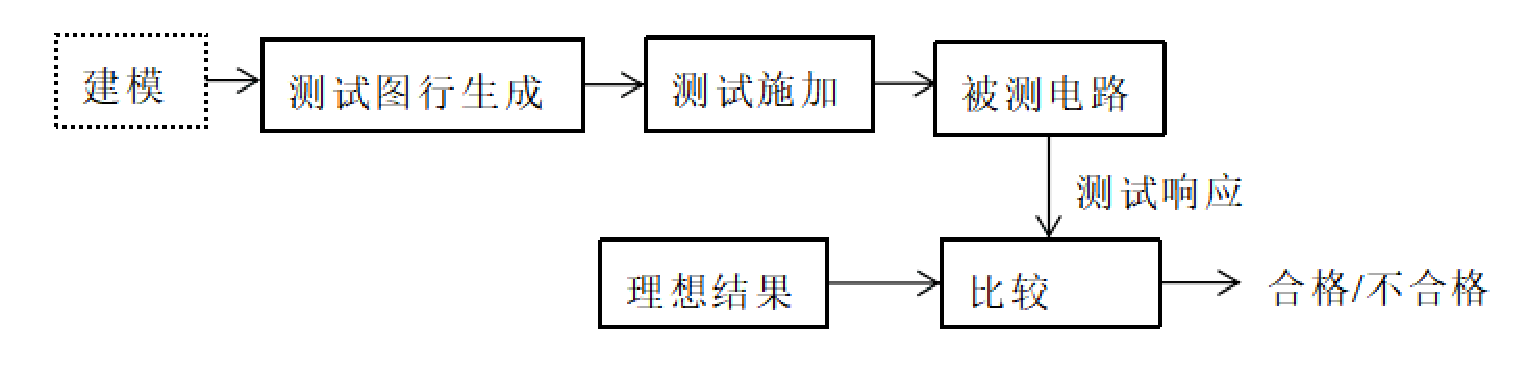
\includegraphics[height=4cm,width=16cm,angle=0,scale=1]{11.eps}
  \vspace*{0\baselineskip}
  \caption{电路测试分析过程}\label{11}
  \vspace{\baselineskip}
     \end{figure}


\subsection{生产测试和功能测试}
生产测试又被称为产品测试,通过对芯片进行缺陷测试或者故障测试以验证其是否符合标准。生产测试方案的制订必须考虑AET性能、测试功耗以及测试时长等影响因子。

功能测试就是对产品的功能进行测试,属于黑盒测试,主要通过检验芯片功能是否符合预期来判断芯片的质量。按照测试过程分类,功能测试可以分为测试施加、测试生成和测试结果验证。按测试生成的方法分类,功能测试可分为穷举测试、伪穷举测试、伪随机测试等。在相关文献\cite{19}中,总结了各类测试方法的特征以及相关术语包括(1)穷举测试、(2)伪穷举测试\cite{20}、(3) 伪随机测试\cite{21}、(4)确定性测试、(5)测试施加\cite{22,23}。

\subsection{可测性设计}

在芯片测试过程中,测试图形生成冗长且困难,于是可测性设计方法就得以发展,其主要是为了解决芯片测试过程所面临的诸多问题,比如测试时长、测试功耗、测试数据量等。因此,在设计芯片的初始阶段就需要考虑如何测试的问题。可测性设计出现于上个世纪70 年代,最先提出的是通过扫描路径\cite{24}对电路进行设计,其中一个典型的应用就是IBM进行的80286研发\cite{25}。

通常有两种方法实现可测性设计。一种方法是专项技术,另一种方法是系统化技术。对于可测性设计,著名学者Bennetts给出了一个定义,给定一个集成电路,通过耗费有限时间和成本完成对其测试,并达到预期的效果,则称此电路是可测的\cite{26}。 实质上这个定义有些含糊,不同的设计者会有不同的解释。例如,关键词“成本”,也许IC制造家为了减少测试成本就会减少这方面的可靠性开支。其流程大致为:在扫描模式下,扫描链移入一个即将被施加到组合逻辑上的测试向量。在系统模式下,经过一个时钟周期,测试向量被施加到组合逻辑上,输出响应在时钟信号下进入触发器。然后扫描链在扫描模式下将组合逻辑的输出响应移出来,同时将下一个测试向量移进去,如此反复进行直至测试完毕。

\section{国内外研究现状}

数据压缩的主要目的是为了减少测试集的数据量,下图\ref{12}给出了测试压缩结构图,由图中可以看出其中包括三个部分,第一个部分是ATE(测试设备),里面存储了压缩激励,第二个部分是CUT (被测电路),第三个部分是压缩的响应。测试过程大致为先将压缩的测试激励经过解压器,还原成为测试向量,然后将已压缩的激励送入到被测芯片上,最后将经过解压器解压缩的测试激励送入被测电路进行测试,捕获电路测试响应,若实际响应与压缩响应一致,则认为此块芯片是合格的。测试激励压缩与测试响应压缩是测试数据压缩的两个部分,根据不同的场景将采取不同的压缩方法,本文所研究的激励压缩要保证压缩之后的测试向量能准确无误地被还原,属于无损压缩。

\begin{figure}[H]
  \centering
  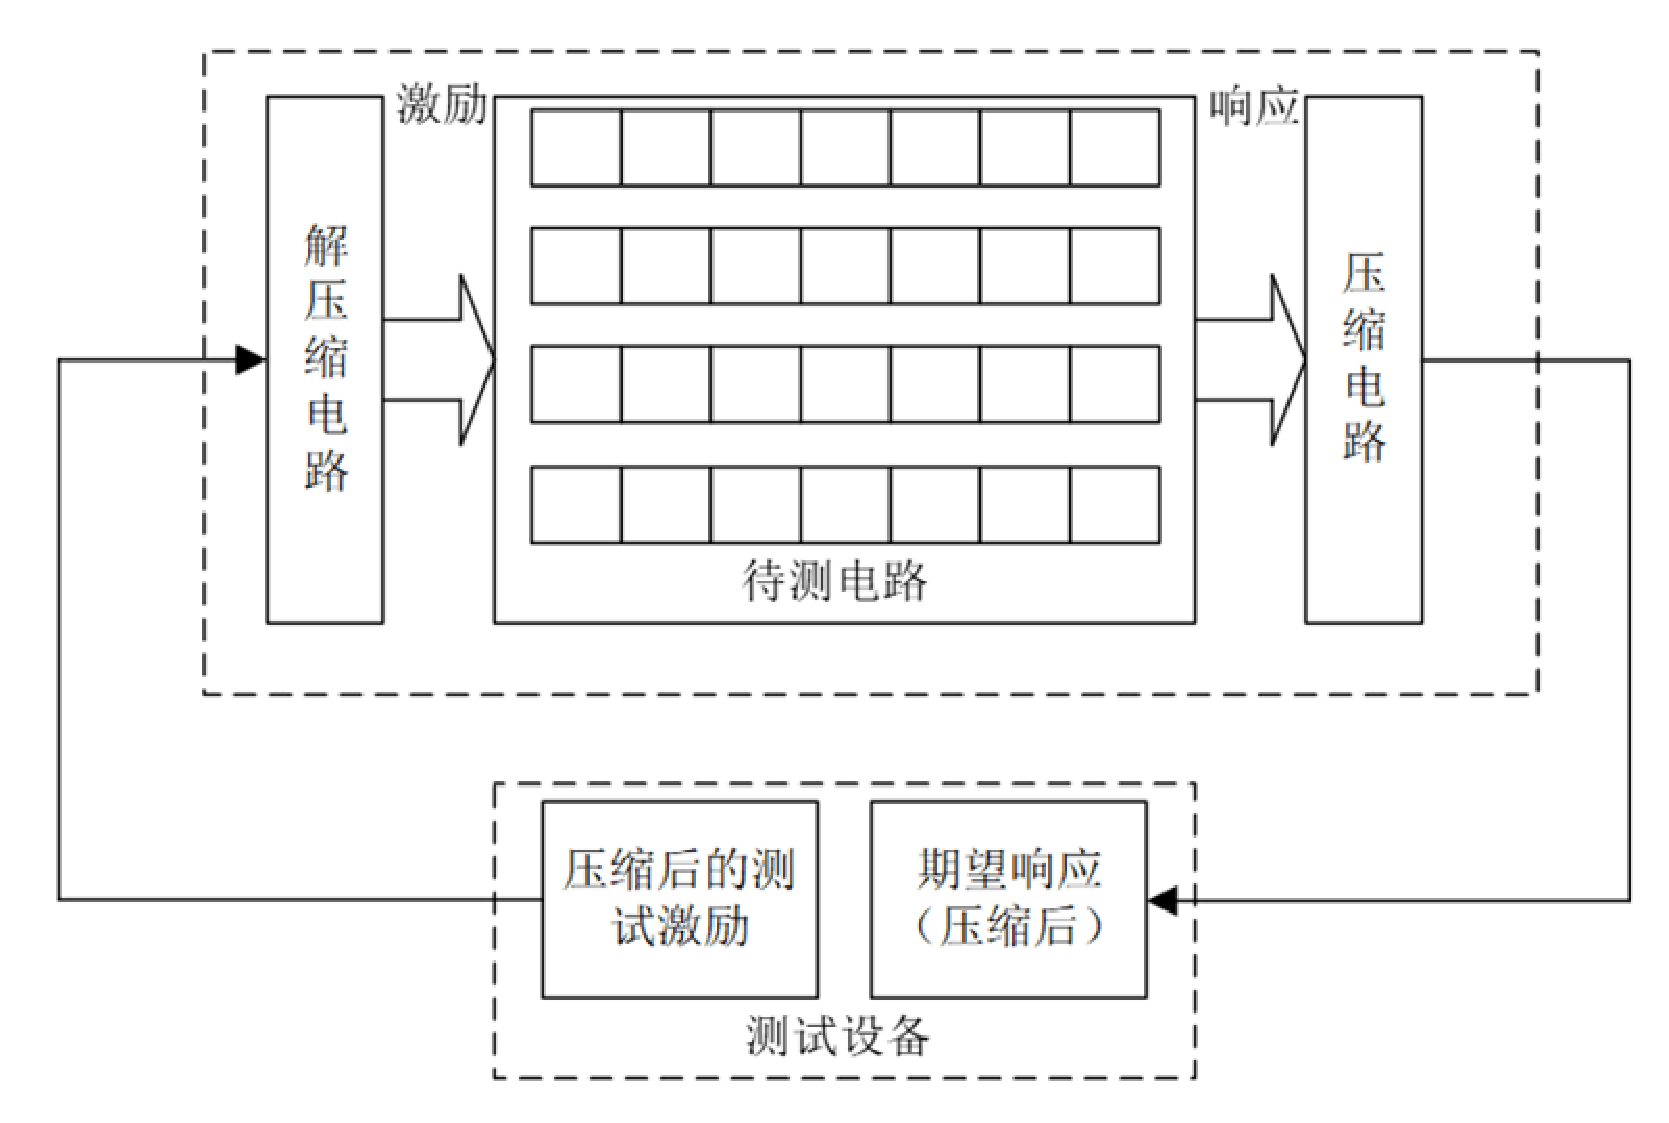
\includegraphics[height=9cm,width=15cm,angle=0,scale=1]{12.eps}
  \caption{数字电路测试压缩结构图}\label{12}
     \end{figure}

测试激励有多种压缩方式,比如编码压缩、线性扫描压缩等等。比较常用的编码有EFDR编码、FDR编码、Huffman编码以及Golomb编码。经过多年发展,近年来提出了拆分压缩这种新型压缩方法。在图像和音频信号的压缩中人们经常使用变换编码的方法,变换编码不是直接对原数据进行压缩,而是将数据以另外一种便于压缩的方式展现出来,通俗地说就是使用一种特殊的码字替换原码字,从而提高压缩率。视频压缩或者音频压缩可以将一些能量较小的数据丢弃,将其转化成为易于压缩的数据,这类压缩方法属于有损压缩。目前,测试激励压缩技术按测试数据存放的位置可以分为两类:内建自测试\cite{27,28}和测试数据压缩。

(1)内建自测试\cite{29}

内建自测试是为了快速地对集成电路进行诊断与测试,为了实现这一功能,一种合适的方式就是将测试规定为一种系统功能。

内建自测试由内建测试(built-in test ,BIT)和自测试(self-test)这两个部分组成。 BIST 是电路(芯片、板或者整机)测试自身的能力。自测试往往不是由硬件实现的,而基于软件实现的,完全基于软件的方式满足集成电路系统级别的要求,会产生诸多缺点,比如降低测试诊断分辨率、延长开发周期与时间、消耗大量的开发成本等等。

内建自测试,是一种使用器件的部分电路来测试器件本身的设计技术,它可以测试功能、结构,但不能测试参数。现在,BIST 技术主要分两种:在线(On-line)\cite{30}和离线(Off-line)。在线,进一步可分为并发在线(Concurrent on-line)和非并发在线(Noconcurrent on-line);离线,进一步可分为功能离线(Functional off-line)和结构离线(Structural on-line)。

在线 BIST,是在能够完成所需要求的情况下进行的。并发在线测试能按照所需要求完成,和其他操作同时进行,这种测试通常用编码技术或复制、比较技术以及线性反馈移位寄存器\cite{31,32}的技术来完成;非并发在线,是指能按照所需要求来完成空闲状态,也叫做后台操作,这种测试通常用软件程序来完成。在线测试是指由其他能够按照要求完成的操作,因此,在线测试能检测实时错误。

离线 BIST\cite{33}是指不能够完成所需要求的情况下进行的,通常使用输出响应分析器和测试向量生成器来完成。功能离线是根据被测器件有什么作用来测试的;结构离线是根据被测器件结构的类型来测试的。由于离线测试没有按照所需要求来完成操作,因此离线测试不能检测实时错误\cite{34}。

BIST 电路一般是由测试图形生成激励、被测电路、数据压缩的电路、进行比较分析的电路、存储理想结果的电路(ROM)和进行自测试控制电路组成,一般结构如图\ref{13}所示。

\begin{figure}[H]
  \centering
  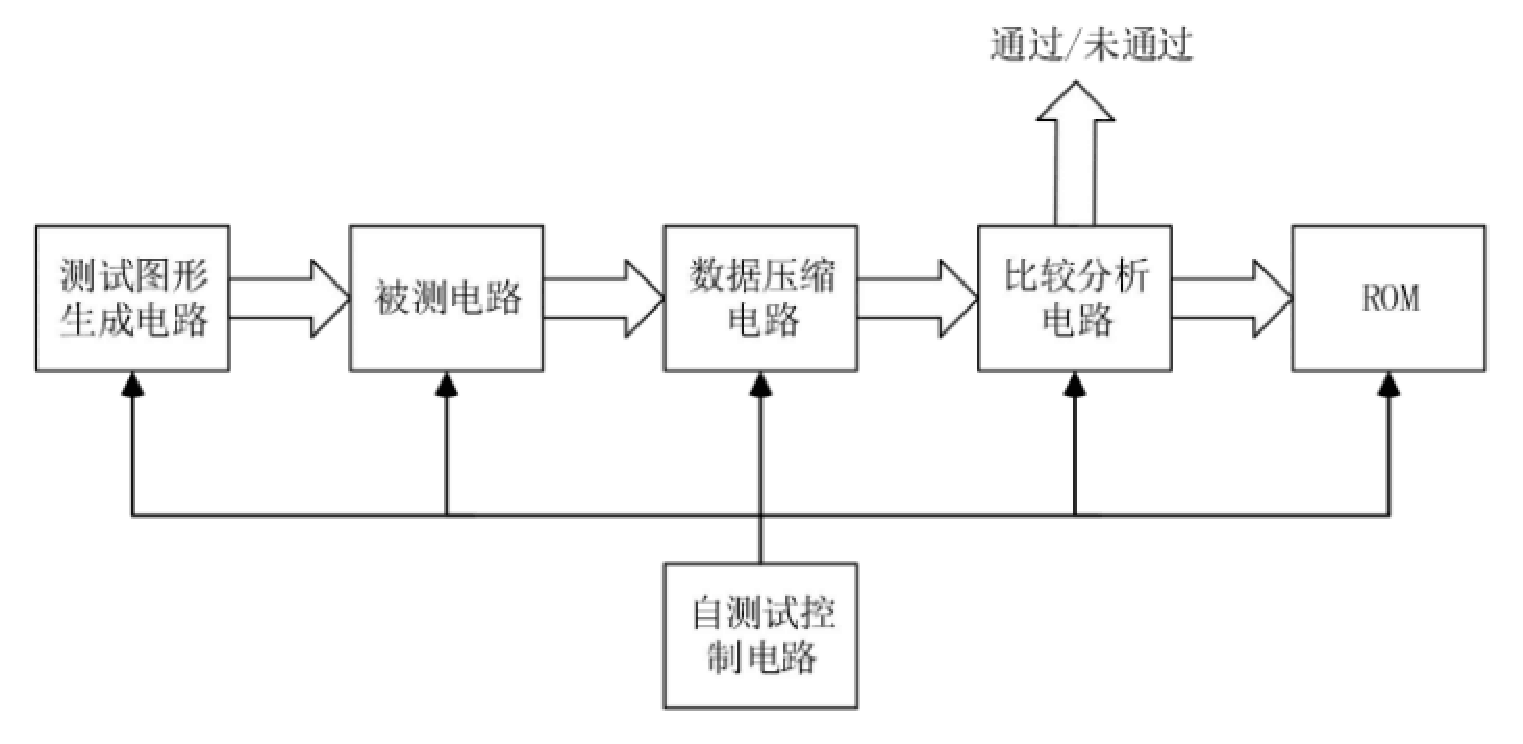
\includegraphics[height=6cm,width=14cm,angle=0,scale=1]{13.eps}
  \caption{内建自测试一般结构}\label{13}
     \end{figure}

推崇大力发展内建自测试主要分为四个目的,第一:为了解决芯片复杂度的问题。当芯片复杂度大大提升时,简单地对测试难集进行拆分是不可能的,并且使用传统化技术解决相对复杂的测试问题相当困难。BIST提供了层次化的解决方法,通过自顶向下的方式对芯片进行测试,同时为了更好地检测一块芯片,判断芯片是否存在质量问题,BIST提供了对加载原件的有效测试,减少了系统级别测试的压力。第二:解决了芯片质量低下的问题。评价芯片质量是一件复杂的任务,首先发生故障的种类不仅取决于系统、芯片,芯片的制造工艺也是不可忽略的因素。通常情况下会将芯片质量定义一个考量标准,比如将芯片的拒收率控制在十万分之1,或者将测试成本控制在一定的范围内。第三:解决了BIST 经济效益的问题。是否采用BIST方案对芯片进行设计,在生产芯片的初始阶段就是一个需要考量的问题。如果是从芯片的层面考虑,使用BIST方案不会节约较多的测试成本,但是BIST往往作用于芯片生产流程的整个生命周期,因此可以带来极为可观的收益。第四:为了解决测试应用问题。近年来,印制板测试主要基于在线测试,在线测试无法首先系统级诊断,只在板从系统拆解之后才是有效的。其次,BIST 为了解决相关测试问题提出了相关优秀的解决方法,比如,在内建自测试时,能够对整机进行测试包括芯片、零件等而避免了昂贵的外设代价,其次对于硬件板和芯片的离线测试,可以使用在系统级别测试。

BIST 的测试向量生成技术可以分为三类:穷举/伪穷举测试法;伪随机测试法;确定性测试法。内建自测是当前广泛应用的可测试性设计方法。其主要思想是测试的向量是由自身获取,不依赖于外部输入\cite{35}。

(2)测试数据压缩

在测试数据压缩方面,国外的起步较早,在1998 年,Jas 和 Touba 提出一种基于码字0编码的编码方案\cite{39},其以较短的固定码字替换较长的0码字串。在 2001 年,Lorse和Sam等人提出来一种基于 Golomb 代码的新的解压缩架构,这种全新的测试压缩方法在编码片上系统中运用广泛,通过使用单个自动测试仪I/O通道驱动片上系统中的多个核,此种解压缩架构又被称为交织解压缩架构\cite{40}。2013年,相关学着基于典型测试序列中0码字的运行分布,提出来一种可变长度的编码方式,并将其称为FDR编码
\cite{41},FDR编码是一种用于对连续0游程编码的方法,若测试集中的1码字较多,会影响压缩率。Maleh 和 Abaji 在FDR编码的基础上加以完善,提出了EFDR\cite{42}的编码方式,此种编码不仅可以对0游程编码,也适用于对1游程编码。随后Usha S. Mehta 和 Kankar S为了在游程编码的基础上进一步提高压缩率,提出了一 种 名 为 Hamming Distance Based Reordering 和 Columnwise Bit Stuffing with Difference Vector (HDR-CBS-DV)的新方案\cite{43}。同时Dasgupta 伊利诺伊大学相关研究人员提出了一种伊利诺伊扫描结构\cite{44}。文献\cite{45}提出了一种新的 LFSR 重播技术,该技术利用电路内部网络的响应作为改变 LFSR 状态的控制信号;文献\cite{46}提出了一种新颖的压缩方法和低成本的解压缩架构,它将基于符号和基于线性的技术的优势结合在一个统一的多核 SoC 解决方案中;为了减少测试响应数据,文献\cite{47}提出了一种新的测试响应压缩方案,称为选择性测试响应集;

国内在数据压缩领域起步较晚,但是也有相关研究成果被提出。文献\cite{48}提出了一种测试数据压缩方法,它结合了基于字典的压缩和基于位掩码的压缩的优点,是一种基于非固定的索引,它使用较短的索引来表示具有较高出现频率的切片,而使用较长的索引来表示具有较低出现频率的切片,然后采用有效的位掩码和基于最大度的 Clique 分区算法来创建尽可能多的兼容切片,文中还提出了一种新的可变前缀双游程代码来压缩不兼容的切片来减少测试数据量;文献\cite{49}提出了一种考虑模式信息维度的基于游程的压缩方法;文献\cite{50} 提出了一种选择性模式压缩方案,可以在基于扫描的测试期间,有最小的测试功率和测试数据量;文献\cite{51}提出了一种二维(空间/时间)压缩技术,可以减少测试数据量并测试知识产权内核扫描测试的应用时间。

通常而言测试数据压缩框架如图1.4所示,ATE上存储了所有的测试数据,购买自动测试仪价格昂贵,因此往往会将测试数据进行压缩节约成本\cite{36,37,38},因此在原有的基础上必须设计解压缩电路,将测试数据还原,其框架图流程图如下图\ref{14}所示。

\begin{figure}[H]
  \centering
  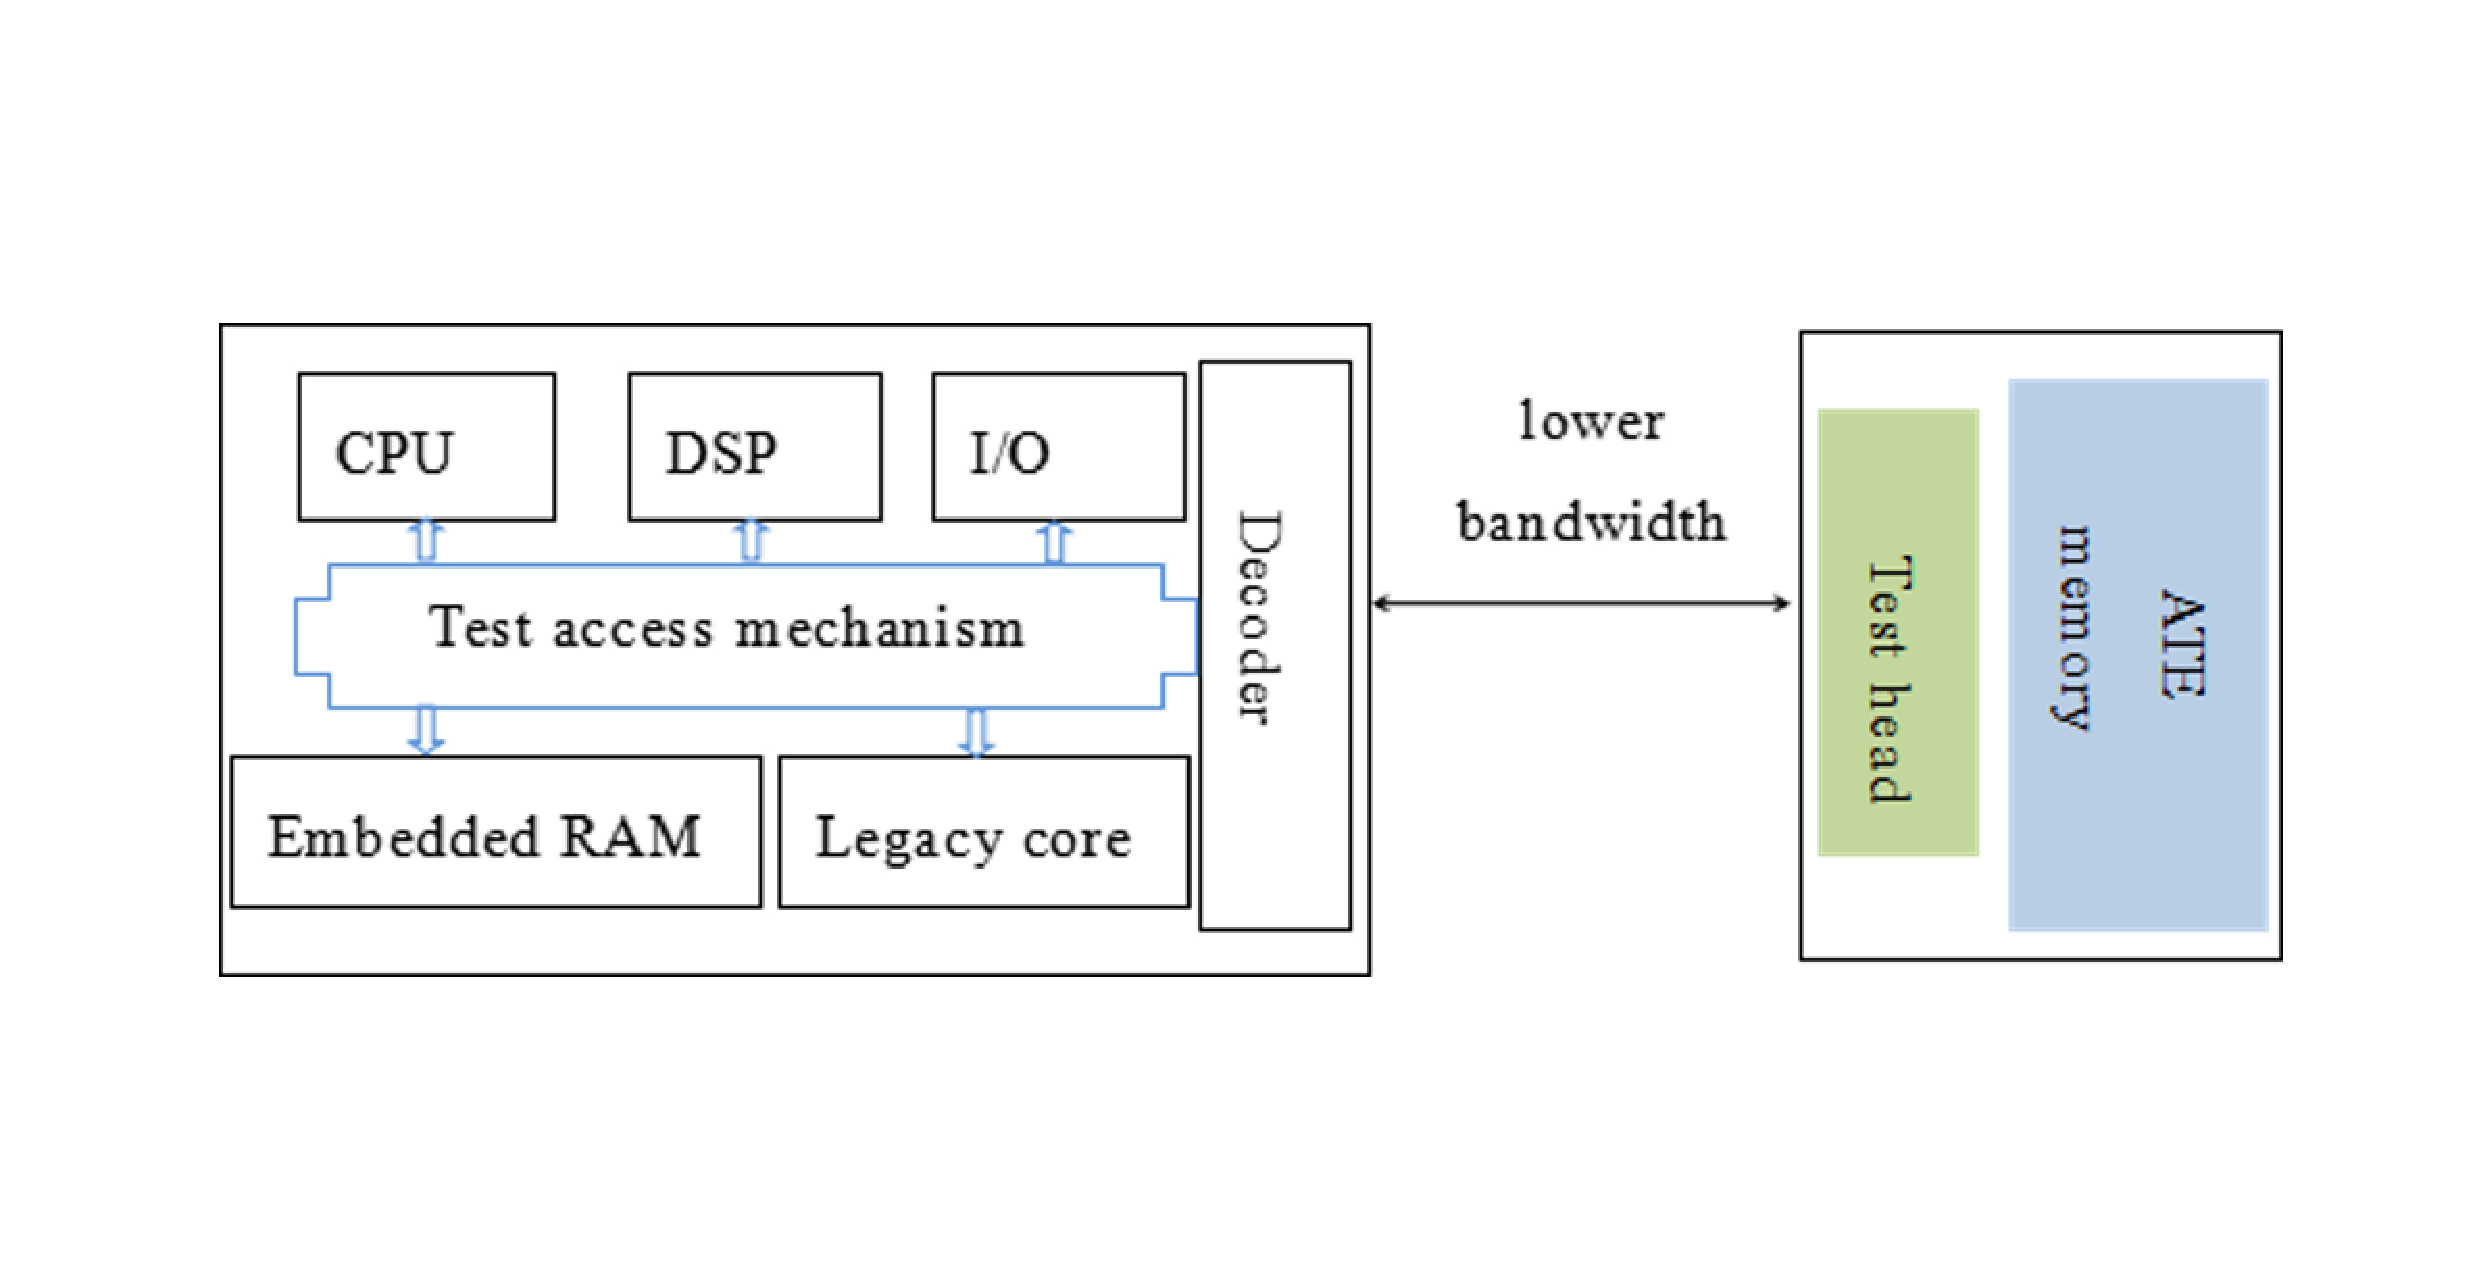
\includegraphics[height=8cm,width=16cm,angle=0,scale=1]{14.eps}
  \caption{TRP框架图}\label{14}
     \end{figure}

\section{本文主要工作及组织结构}

本文在拆分压缩的基础上,主要针对基向量的生成方式进行了研究。由于主分量集是由基向量确定的,因此基向量选取的好坏将导致最终压缩率的高低。生成主分量集的方法有哈达码变换、K-L 变换、离散余弦变换等,本文在拆分压缩的基础上,提出来两种基向量生成算法,一种是将测试集预填充后,以列向量间欧几里得距离最大为原则选取基向量,第二种是使用聚类算法生成实验所需的基向量。同时本文还将聚类算法与位翻转算法进行结合进一步提高压缩率。这三种方法针对压缩率都达到了较好效果。

文本总共分为五个章节阐述自己的工作:

第一章是绪论部分,首先介绍了集成电路发展的背景以及电路测试的相关先修知识,其次就国内外研究现状进行分析最后总结本文的组织结构。

第二章主要就常用的压缩方法做了详细地介绍。第一部分讲解了编码压缩技术,包括游程编码、字典编码以及统计编码。第二部分就基线性解压缩和广播扫描两种非编码压缩方法做出了相应的分析与阐述,最后介绍了拆分压缩技术和哈达码变换,并对哈达码变换的优缺点进行了分析。

第三章重点介绍了使用预填充策略处理数据集的方法,包括填充规则、基向量的选取等步骤。

第四章详细介绍了相关聚类算法以及如何将聚类算法应用于测试电路压缩的具体步骤。同时本章进行了大量的实验用于验证此方法的有效性,并通过动态选取基向量数,较好地反映出压缩率与基向量个数之间的线性关系。

第五章介绍了位翻转算法的相关概念与计算流程,并将kmeans++算法结合位翻转算法进一步提高压缩率。

最后总结全文,并对该研究工作中的问题进行了展望。

% !Mode:: "TeX:UTF-8"

\chapter{测试向量压缩}

集成电路的发展日新月异,导致体积急剧减小的芯片上集成的晶体管数目却迅速增加,测试芯片需要的巨大测试数据集不仅提高了测试功耗,更增加了测试时间以及存储开销。数据压缩可以有效地解决上述问题。本章首先讲述电路可测性基础理论,然后就编码压缩方法、非编码压缩方法以及拆分压缩做进一步阐述。

\section{测试压缩原理}

测试压缩的主要目的在于减少测试数据量、降低测试时间以及节约最终的芯片制造成本。测试数据压缩可以采用多种方式,其目的均是为了降低原测试集中的比特位。当前比较常用的素具压缩算法有基于编码的数据压缩算法,基于线性扫描的数据压缩算法以及基于拆分测试集的数据压缩算法。

测试数据压缩有别于视频压缩,视频压缩属于有损压缩,可以丢弃残差集。当丢弃部分数据之后,并不会有损人们的视觉或者听觉效果。测试数据压缩属于无损压缩,压缩之后的数据需要被无差错地还原。测试集由0、1以及$X$位(无关位)组成,$X$位的产生和自动生成算法有关,测试集中具有较多的无关位,部分电路测试集甚至可达80\%以上。在测试压缩中,$X$根据特定的场景被任意地填充为0 或1,压缩率往往随着的无关位的增加而提高。本文主要针对测试激励进行相关压缩算法的研究,常见的测试激励压缩方法有广播扫描、编码压缩以及线性解压缩。 在测试响应压缩领域也有很多压缩方法,常用的有奇偶校验、特征分析等压缩方法。其中通过线性反馈移位寄存器(LFSR)来对特征进行分析是十分普遍的现象\cite{52,53}。

\section{编码压缩}

编码压缩技术是指将某一种特定码字的编码用其他的码字表示,以减少实际码字的位数,从而达到“压缩”的效果。编码压缩大体可分为三类:第一类是信息源的统计特性分为变换编码、子带编码等。第二类是根据人眼视觉特性,采取小波变换、基于方向滤波的图像编码等。第三类是根据传递景物特征编码。采用不同的编码方式对相同的数据集编码方法,所达到的压缩率是不一样。压缩通用流程如下图\ref{25} 所示。

\begin{figure}[H]
  \centering
  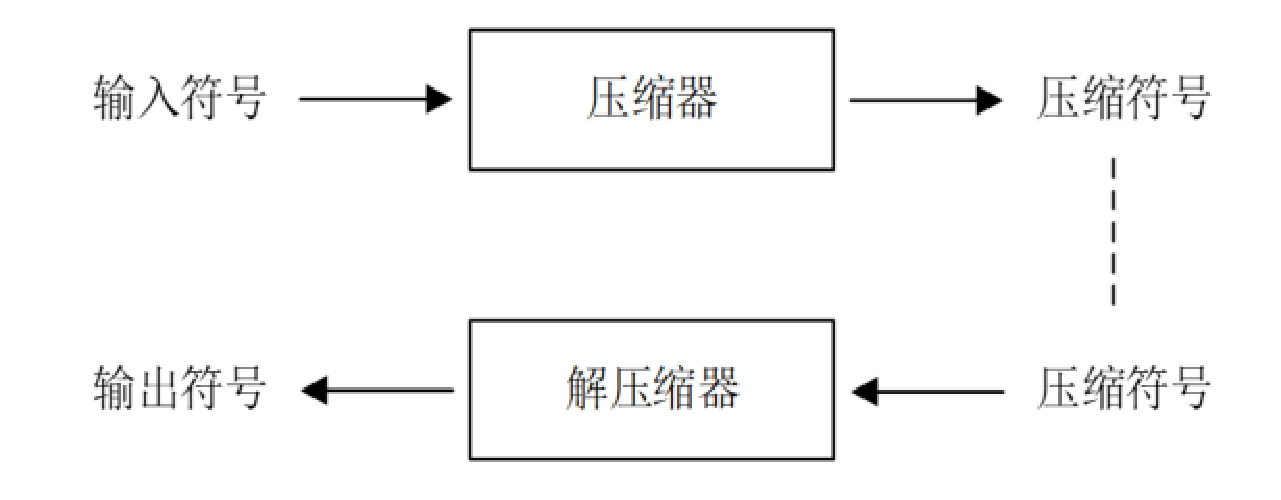
\includegraphics[height=4cm,width=12cm,angle=0,scale=1]{21.eps}
  \caption{压缩通用流程图}\label{25}
     \end{figure}

\subsection{游程编码}

游程编码,又称运行长度编码,指由一连串字符(或信号采样值)组成的数字编码。该编码属于无损压缩编码,其广泛应用于数据压缩领域,同时游程编码\cite{54}也是作为二值图的重要编码方法之一。目前在数据压缩算法中较为常用的游程编码有Golomb 编码\cite{55}、FDR编码\cite{56}、EFDR 编码\cite{57}以及交替游程编码(ALT-FDR)\cite{58}。根据游程编码进行分类,有单游程编码和双游程编码两种方式。其中单游程编码中比较常见的有FDR 编码,FDR 编码的基本规则是,只对游程中 0 的长串进行编码,根据 0 串的长度会生成唯一的码字,当 0 串越长所对应的码字相对于原串而言就越短,从而压缩率也越高,对于游程中出现的 1 比特位,我们使用使用码字 00 来进行编码,因此当测试集中1比特位较多时,不建议使用FDR编码,EFDR的效果更佳。下表
\ref{tabl2}为FDR的前几组编码。

EFDR编码不仅可以使用较短的码字对连续的0码字进行编码,对于连续的1码字也同样适用。当测试集的跳变数越少,使用EFDR编码所能达到的压缩率就越高。下表\ref{tabl3}为EFDR前一部分编码规则。下面举例说明EFDR的的压缩流程。测试向量$T={1111110 0000001 111111111111110}$,根据EFDR码表可将其划分为三个游程,其长度分别为{6,6,14}。使用EFDR编码压缩后测试向量变为{11010 01010 1110111},减少了12位。
\begin{table}[H]
\centering
\caption{FDR编码表}\label{tabl2}
\begin{tabular}{p{1.6cm}p{2.7cm}<{\centering}p{2.7cm}<{\centering}p{3cm}<{\centering}p{3.6cm}<{\centering}}
\toprule
\textbf{组}&	\textbf{游程长度}&     \textbf{前缀}&   \textbf{尾部}&   \textbf{码字}\\
\midrule
\multirow{2}{*}{A1} & 0 & \multirow{2}{*}{0} & 0 & 00 \\
& 1 &  & 1 & 01 \\
\hline
\multirow{4}{*}{A2} & 2 & \multirow{4}{*}{10} & 00 & 1000 \\
& 3 &  & 01 & 1001 \\
& 4 &  & 10 & 1010 \\
& 5 &  & 11 & 1011 \\
\hline
\multirow{8}{*}{A3} & 6 & \multirow{8}{*}{110} & 000 & 110000 \\
& 7 &  & 001 & 110001 \\
& 8 &  & 010 & 110010 \\
& 9 &  & 011 & 110011 \\
& 10 &  & 100 & 110100 \\
& 11 &  & 101 & 110101 \\
& 12 &  & 110 & 110110 \\
& 13 &  & 111 & 110111 \\
\bottomrule
\end{tabular}
\end{table}

\begin{table}[H]
\centering
\caption{EFDR编码表}\label{tabl3}
\begin{tabular}{p{1.6cm}p{1.6cm}<{\centering}p{2.2cm}<{\centering}p{2.2cm}<{\centering}p{3cm}<{\centering}p{3cm}<{\centering}}
\toprule
\textbf{组}&	\textbf{游程长度}&     \textbf{前缀}&   \textbf{尾部}&   \textbf{0油程}&   \textbf{1油程}\\
\midrule
\multirow{2}{*}{A1} & 1 & \multirow{2}{*}{0} & 0 & 000& 100 \\
& 2 &  & 1 & 001 & 101 \\
\hline
\multirow{4}{*}{A2} & 3 & \multirow{4}{*}{10} & 00 & 01000& 11000 \\
& 4 &  & 01 & 01001 & 11001\\
& 5 &  & 10 & 01010 & 11010 \\
& 6 &  & 11 & 01011 & 11011 \\
\hline
\multirow{8}{*}{A3} & 7 & \multirow{8}{*}{110} & 000 & 0110000 & 1110000 \\
& 8 &  & 001 & 0110001 & 1110001 \\
& 9 &  & 010 & 0110010 & 1110010 \\
& 10 &  & 011 & 0110011 & 1110011 \\
& 11 &  & 100 & 0110100 & 1110100 \\
& 12 &  & 101 & 0110101 & 1110101 \\
& 13 &  & 110 & 0110110 & 1110110 \\
& 14 &  & 111 & 0110111 & 1110111 \\
\bottomrule
\end{tabular}
\end{table}

\subsection{字典编码}

字典编码是一种随着数据流本身的特点动态地构建适合该数据流的编码,在文本压缩、音频压缩中应用比较广泛。相比于统计编码,它的实现既不需要用到统计的方法,也不需要用到变长码的方式,而是从数据流中选择多个字符串,利用字典的方式,对其进行编码压缩。字典编码根据是否可以通过静态的方式对数据流中的字符串进行保存分为非自适应LZ编码和自适应LZ编码。

下图\ref{26}是使用完全字典压缩方法的原理图,图中$b$代表测试通道的数量。$n$代表扫描链的数量,$n$的值往往大于$b$,$n$与$b$的比值越大,每一条扫描链的长度就越。使用此方法能提高加载测试向量的效率,减少测试时间。其不足之处在于,若使用完全字典的方式,需要存储巨大的数据量,增大硬件开销。因此部分学者使用部分字典的方式,对不在字典中的数据进行纠错以达到控制字典的大小,通过在硬件代价与纠错成本之间进行权衡,从而达到一定的压缩率。

\begin{figure}[H]
  \centering
  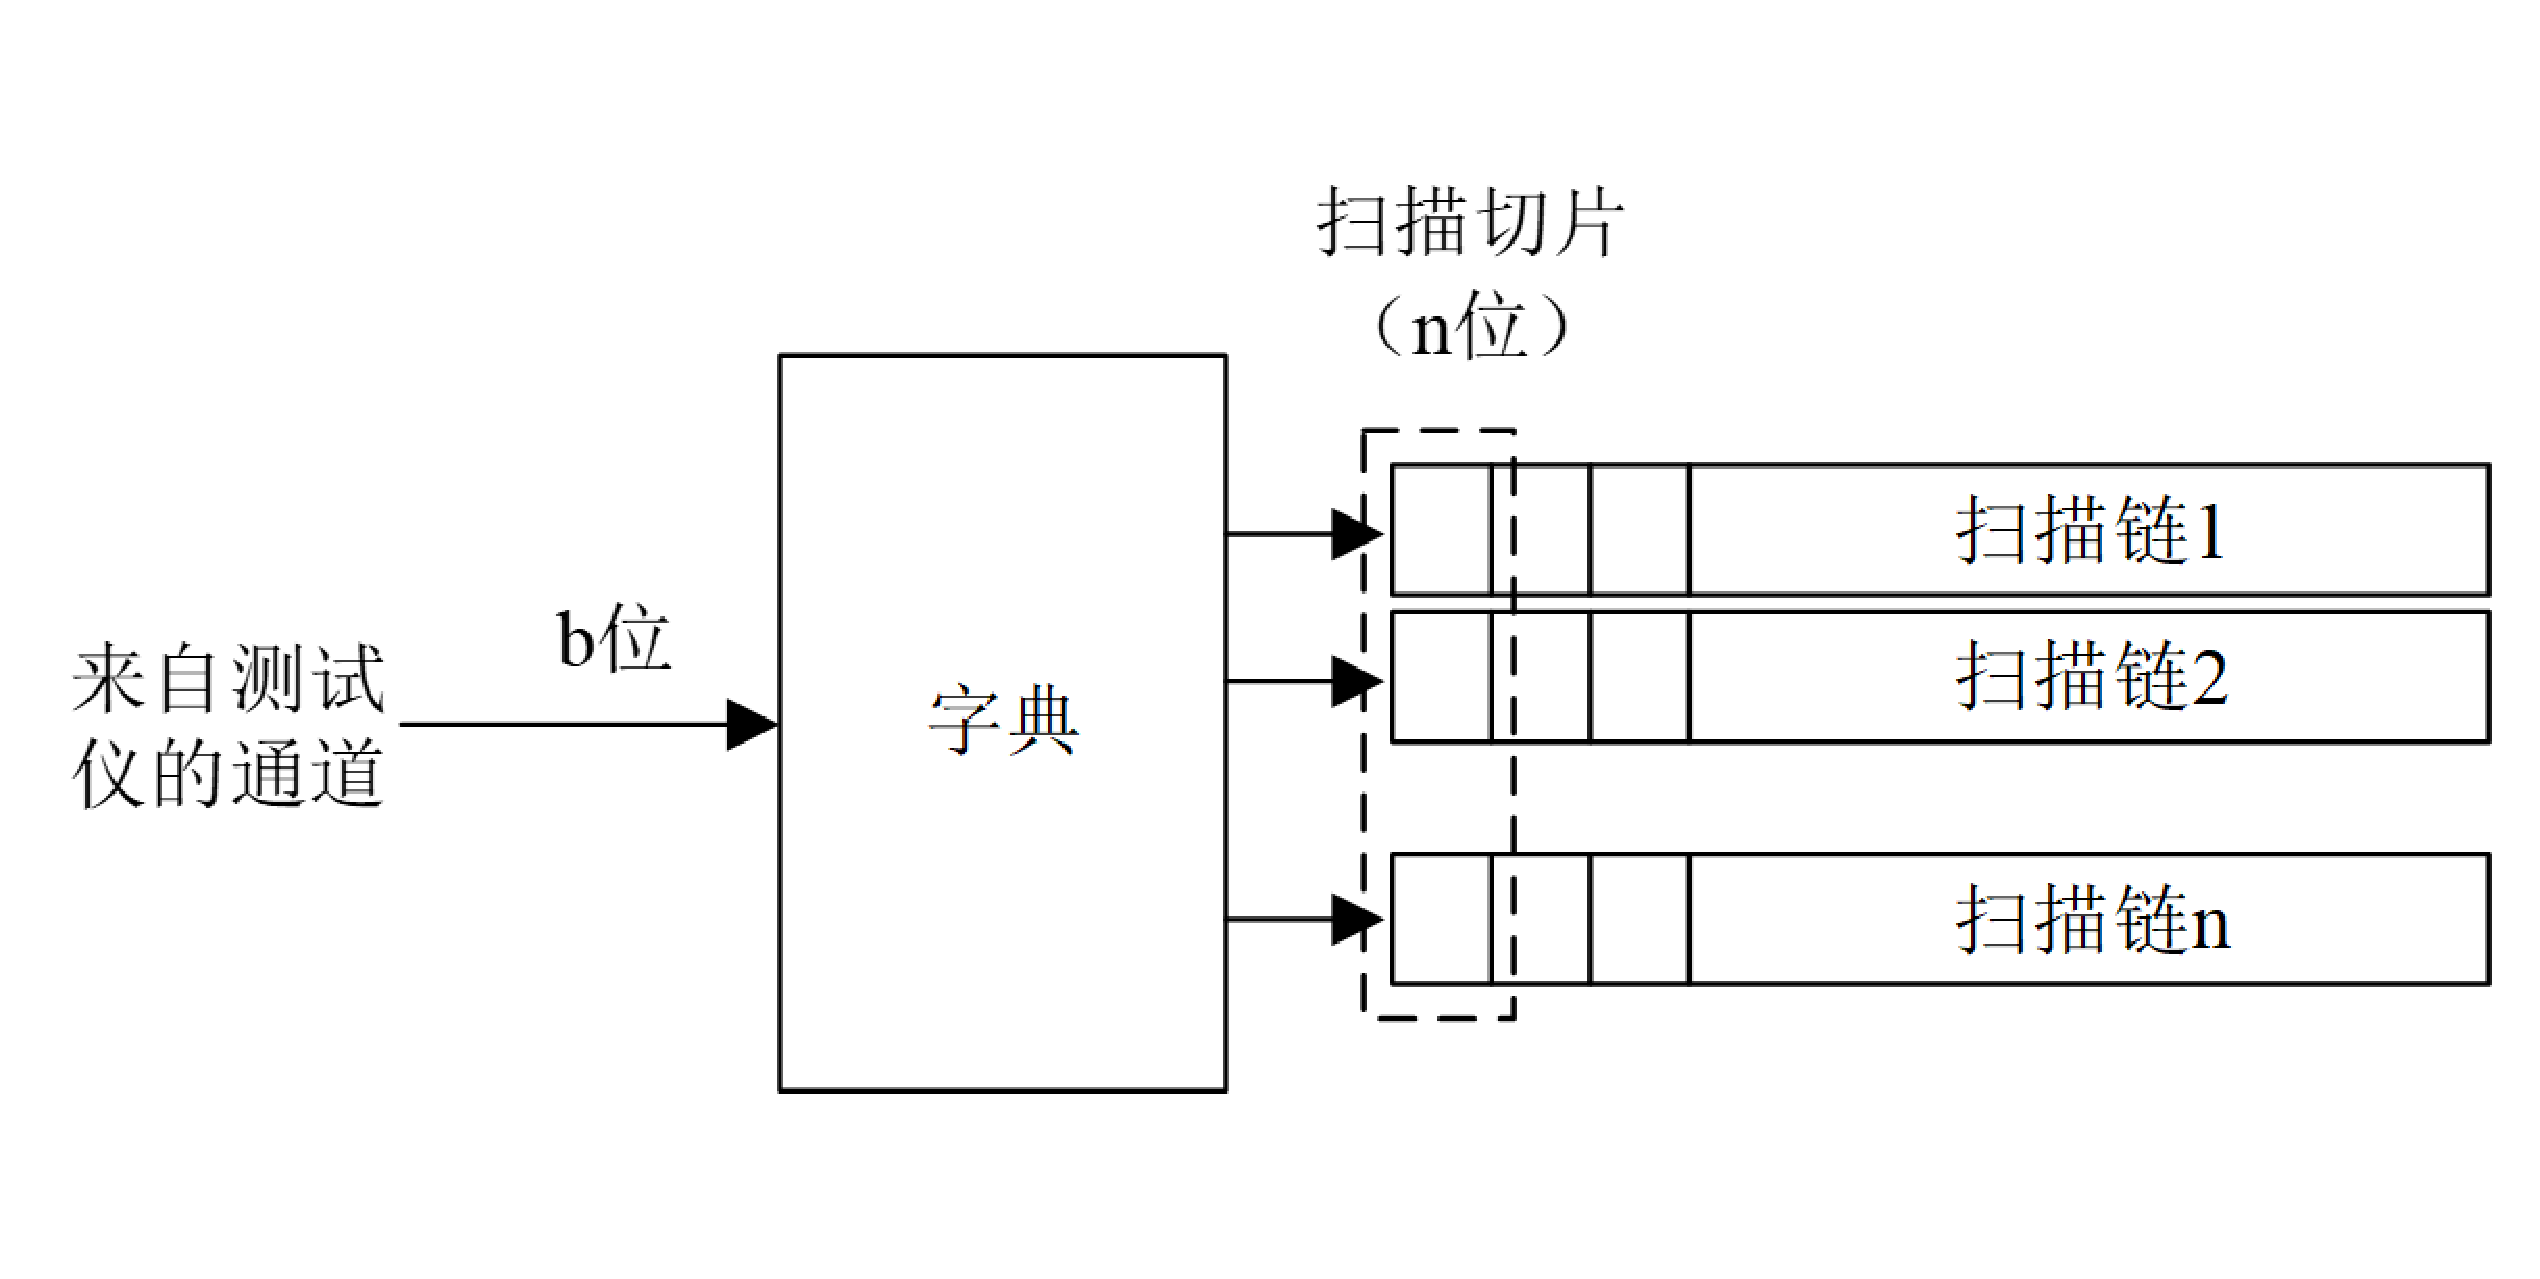
\includegraphics[height=7cm,width=14cm,angle=0,scale=1]{26.eps}
  \caption{字典压缩方法}\label{26}
     \end{figure}

\subsection{统计编码}

统计编码是一种在测试数据压缩中广泛运用的压缩方法。其本质就是通过某种方式将原数据集拆分为一个个数据块并进行数学统计,将重复率高的数据块以短码字编码,从而达到数据压缩的目的。假定原数据集合为$X$,先按照一定的规则对$X$ 进行分块或者分类,统计出相同块 的数量,然后进行编码。被大家广为熟知的有霍夫曼编码\cite{59}。 霍夫曼编码通过构造霍夫曼树,将原数据集合拆分成为等长的信源符号。然后统计出相同的信源符号的个数并排序,将重复次数多的部分用短码字描述,重复次数少的部分用长码字描述,从而减少原测试集中的比特位,压缩测试数据。

部分学者对Huffman编码进行改进,衍生出譬如最优选择哈夫曼(OP-SHC)\cite{60}以及多级哈夫曼\cite{61,62,63}等编码方式。下面将举例说明如何使用霍夫曼编码,下图中框中为本例使用的数据集,总共有80位。对于初始数据集的处理,首先将其划分成为4 位为一组的比特块,然后将每一个比特块出现的频率进行统计,如下表\ref{tabl5} 所示,可以发现表中1010、0000、1111三种数据块出现的频率最高。最后对出现次数最多比特块进行霍夫曼编码,如下图\ref{27}所示。对于未编码的块则需要在原有码字之前加上111,通过使用霍夫曼编码可将原数据集中的数据压缩38.8\%。

\begin{table}[H]
\centering
\caption{测试集的划分和各种块出现的频率}\label{tabl5}
\begin{tabular}{p{7cm}<{\centering}p{2.7cm}<{\centering}p{2.7cm}<{\centering}}
\toprule
\textbf{测试集T}&	\textbf{不同的块}&     \textbf{频率}\\
\midrule
1010 0000 1010 1111 &1010 & 9/20\\
1111 0000 1010 0001	&0000&5/20\\
1010 0000 0010 1010	&1111&3/20\\
0000 1010 1010 0000	&0001&2/20\\
1010 1111 1010 0001	&0010&1/20\\
\bottomrule
\end{tabular}
\end{table}

\begin{figure}[H]
  \centering
  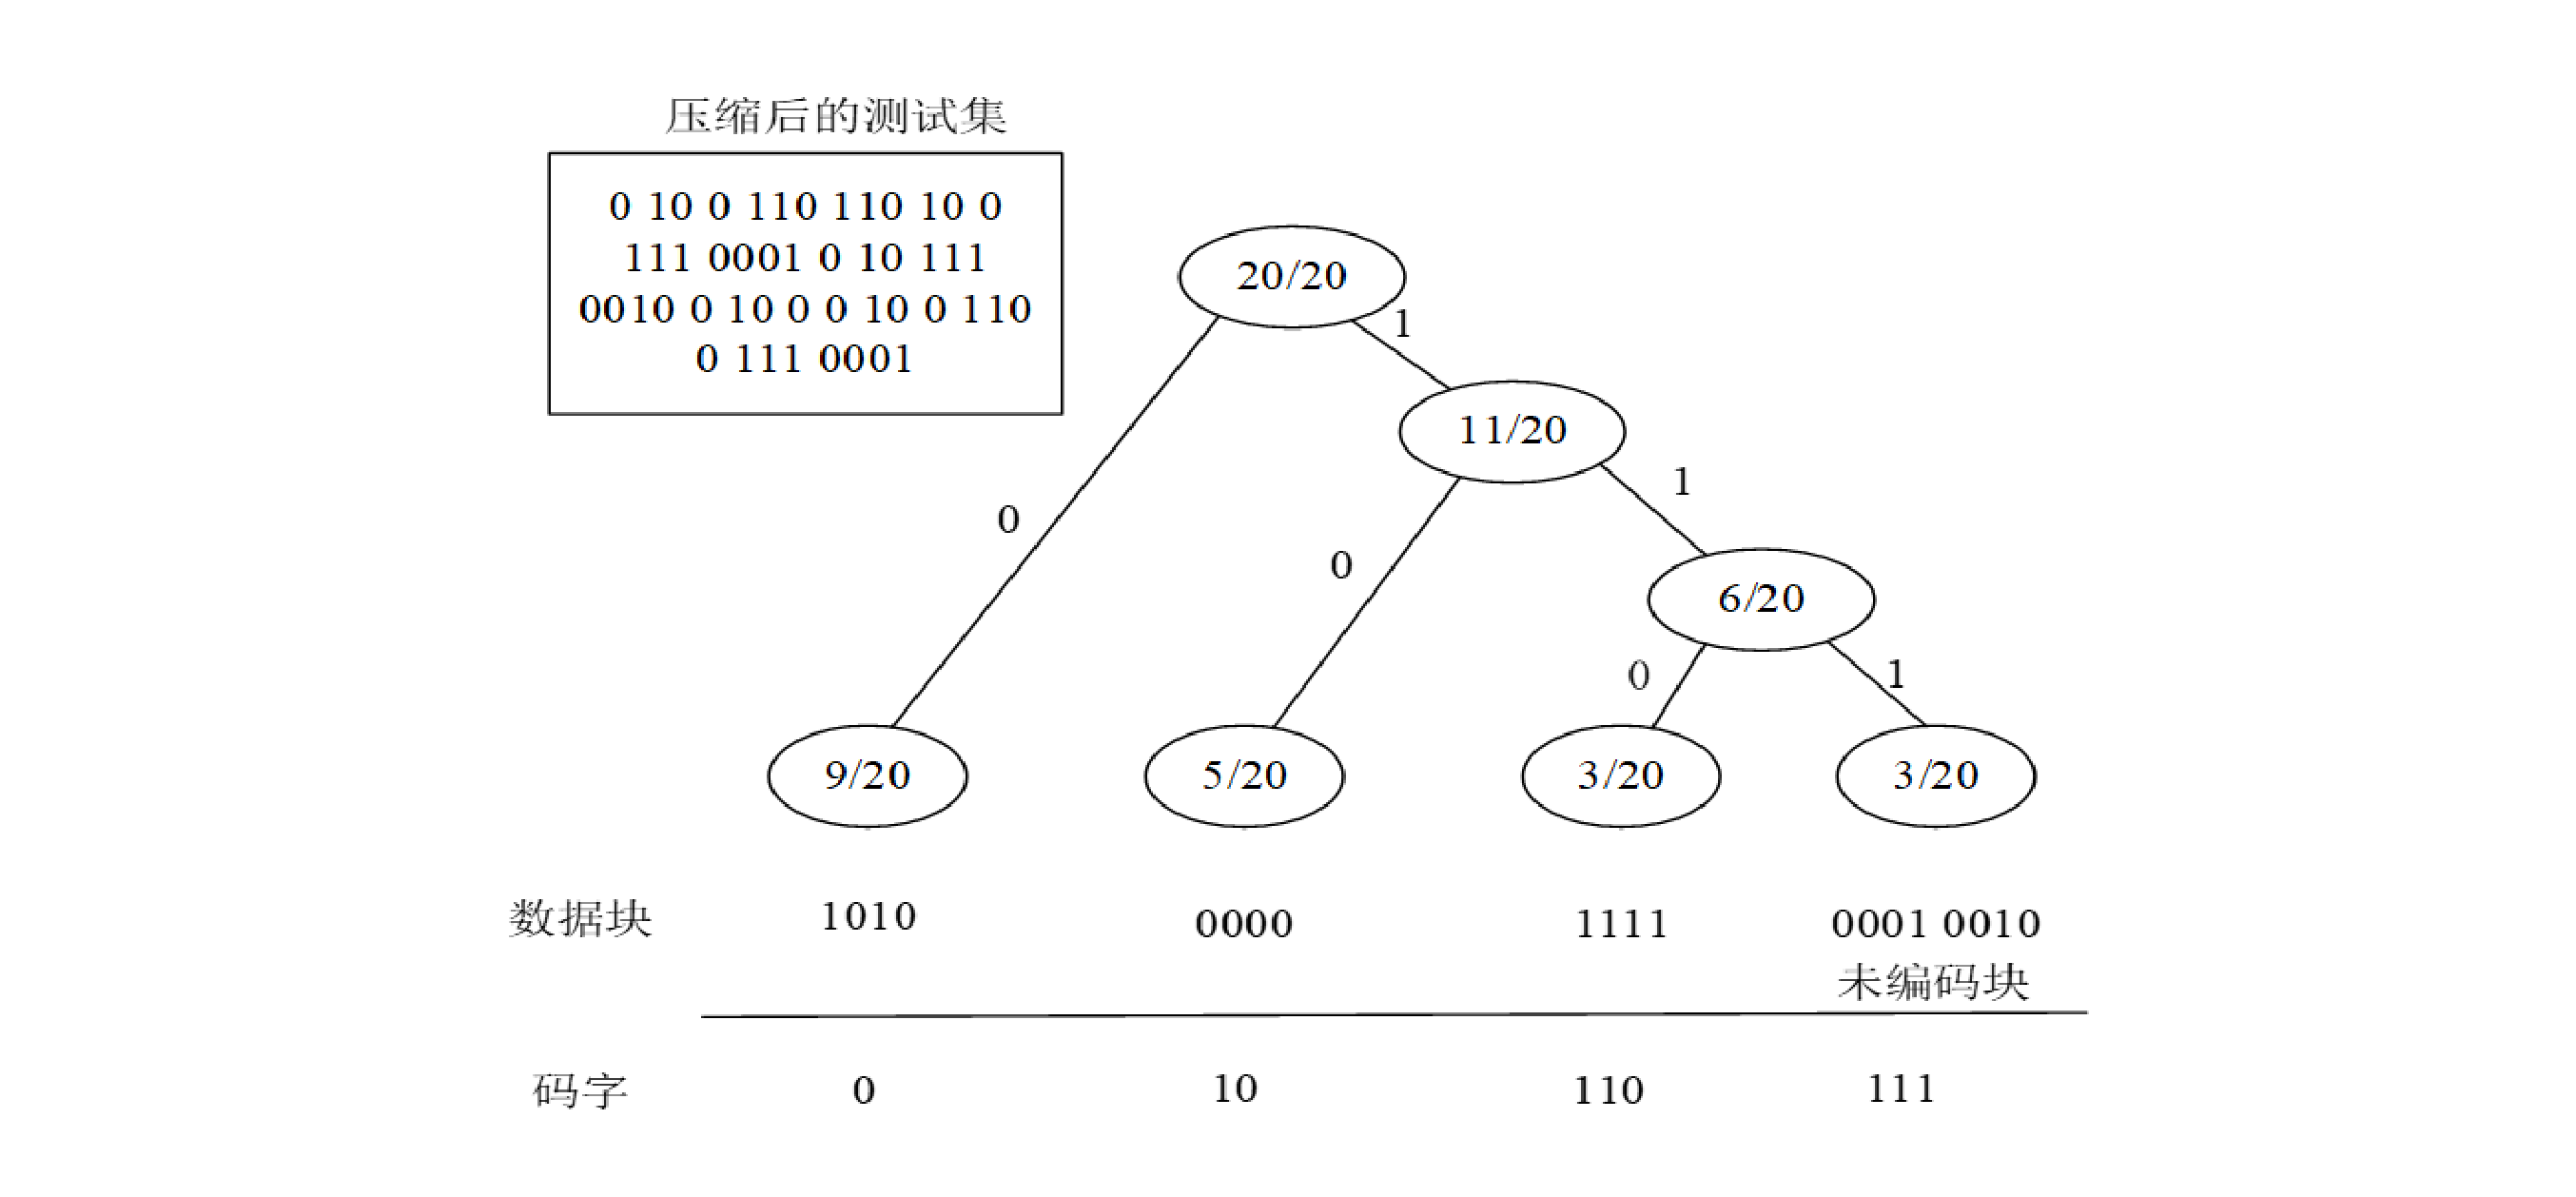
\includegraphics[height=10cm,width=16cm,angle=0,scale=1]{27.eps}
  \caption{最优选择哈夫曼编码}\label{27}
     \end{figure}

除了上文介绍的几种编码外,9C\cite{64}、多层复制\cite{65}、块合并\cite{66}、BM-8C\cite{67}、SVC\cite{68}、 选择扫描切片\cite{69} 等编码在数据压缩领域也较为常用。

\section{非编码压缩}

\subsection{基于线性解压缩}

线性解压缩器是一种包含了D触发器、RS触发器以及异或门的解压缩结构,如下图\ref{28}所示,其由四部分组成,左边是拥有$b$个通道的代码测试仪,经过LFSR到达了组合线性网络,然后将LFSR中的数据扩展至右边的$n$条扫描链中,每一条扫描链中有$m$位数据,因此需要$b(q+m)$ 个比特位的数据才能产生一个测试集。当对测试集解压缩时,线性反馈移位寄存器会将压缩数据还原为原测试集合并进行初始化,等待时钟周期的到来再将数据传送至扫描链。

\begin{figure}[H]
  \vspace{\baselineskip}
  \centering
  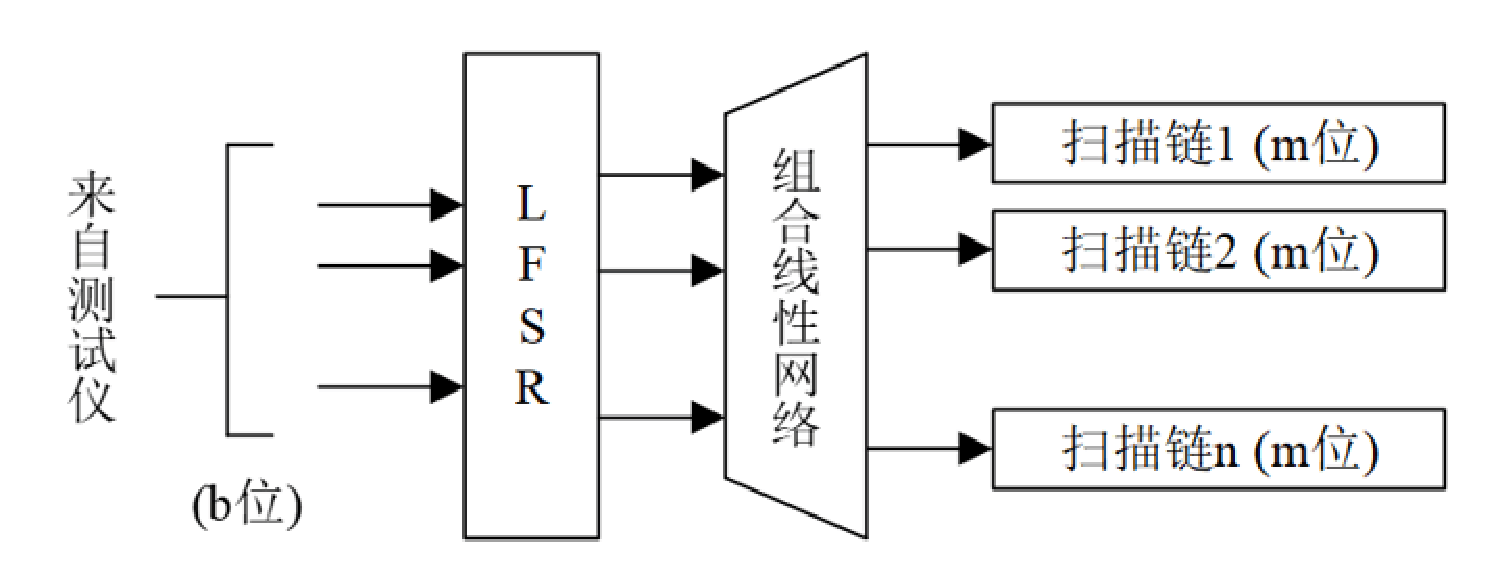
\includegraphics[height=4cm,width=14cm,angle=0,scale=1]{28.eps}
  \vspace{\baselineskip}
  \caption{时序线性解压器}\label{28}
     \end{figure}

\subsection{基于广播扫描}

“广播扫描”从字面上的意思来理解,就是使用广播的方式将数据施加多条扫描链,可以类比于IO多路复用的方式,即使用一个线程监听多个socket, 在本实验中即驱动多个扫描链。其中Illinois扫描结构\cite{70}比较具有代表性,其结构如图\ref{29}所示。

\begin{figure}[H]
  \centering
  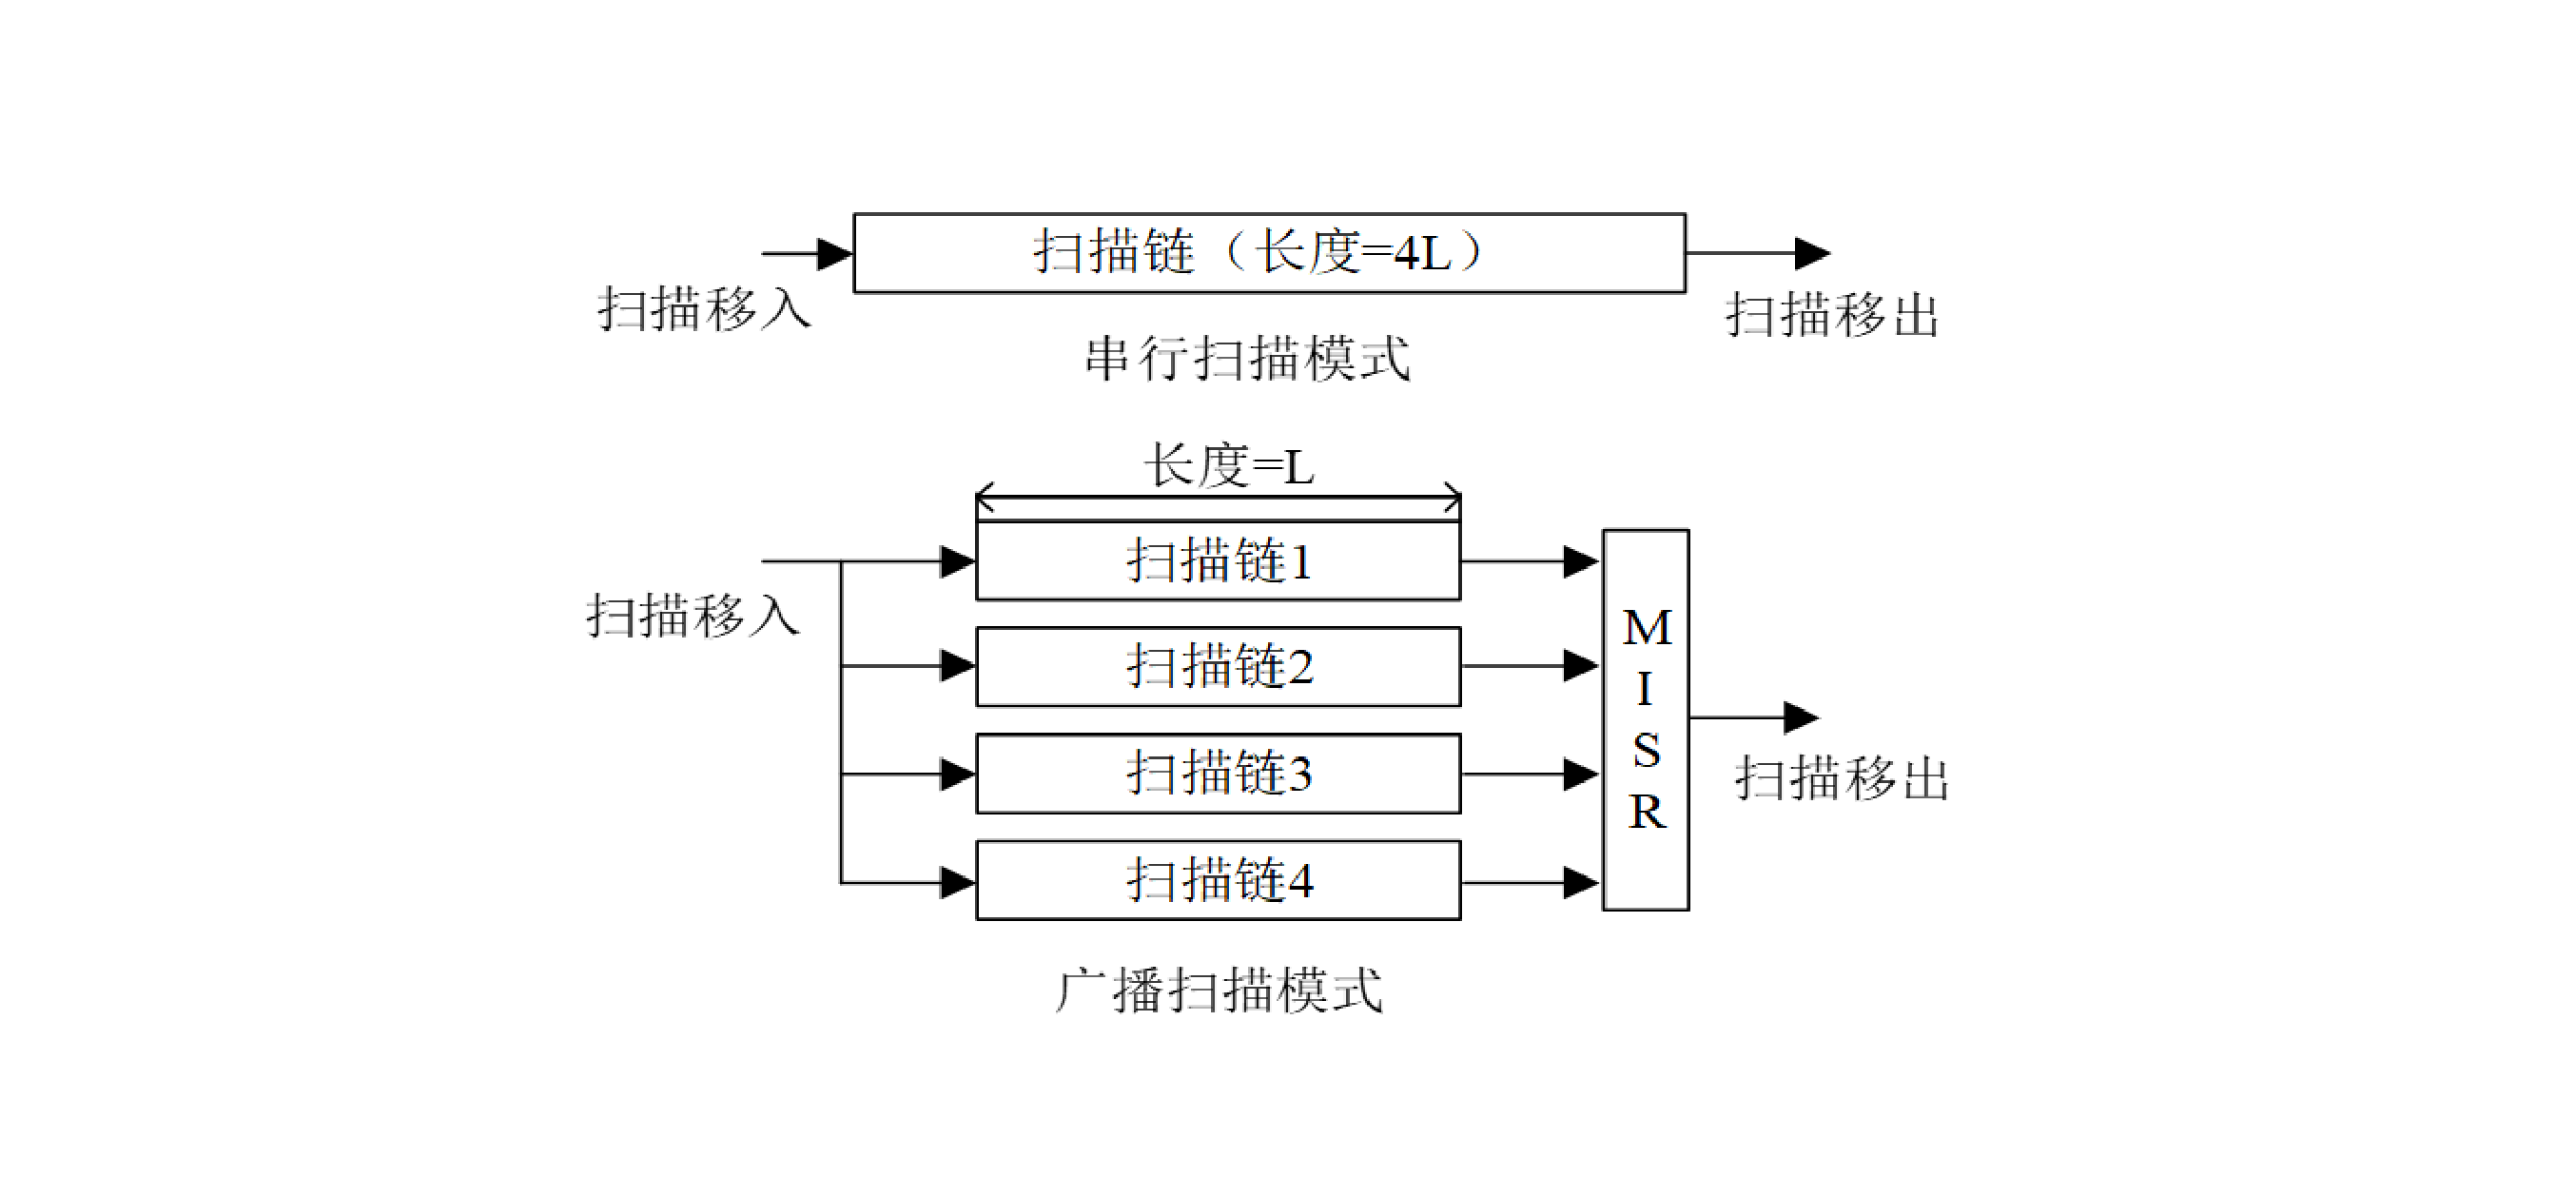
\includegraphics[height=8cm,width=16cm,angle=0,scale=1]{29.eps}
  \caption{广播扫描结构}\label{29}
     \end{figure}

广播扫描模式较传统扫描模式不同点在于,广播扫描模式将扫描链进行拆分并将扫描链连接到同一输入。上图的原始扫描链为$4L$,每一个子扫描链都为$L$,这可能会导致故障遗漏,因此,需要结合串行扫描模式才能排查出电路中存在的故障,提高故障覆盖率。广播扫描模式由于扫描链之间会存在相等值,将导致某些故障无法检测,因此多输入扫描链的方式应运而生。其改进的措施为先将扫描链分为多组,每一组的输入端均不相同但组内数据相容,最终确保每一组故障覆盖率达标。 其次采取重新配置广播扫描链的结构或者降低测试过程所需的功耗也可用来提高压缩率。

\section{哈达码变换}

\subsection{基本原理}

哈达码变换是利用哈达码矩阵作为变换矩阵,将原有数据表示为新数据的一种变换方式。自然界有很多的信号,例如图像、声音、视频等经过变换编码后进行高倍率的压缩。哈达码变换使用通式$Y=HX$ 表示,其中 $X$ 和 $Y$ 均是一列向量,$H$ 为哈达码矩阵。哈达码变换已广泛应用于视频和音频编码中,由于其硬件代价低实现简单的特点,也被人们应用于测试数据压缩。与多媒体数据的压缩的不同之处是,激励压缩属于无损压缩。

\subsection{哈达码矩阵以及变换的基本流程}

哈达码变换中使用的矩阵由-1和1组成,这种天然的特性非常适用于电路测试,矩阵中1等价于测试集中的1比特位,-1等价于测试集中的0 比特位。哈达码矩阵可以被递归定义:

\begin{equation}
H(k)
=
\left[
\begin{array}{cc}
    H(k-1)&H(k-1)\\
    H(k-1)&-H(k-1)\\
\end{array}
\right]
,k=1,2,....,n,
\end{equation}

其中H(0)=1,根据上述通式,当$k=1$以及$k=2$时有下列矩阵:

\begin{equation}
H(1)
=
\left[
\begin{array}{cc}
    1&1\\
    1&-1\\
\end{array}
\right]
\end{equation}

\begin{equation}
H(2)
=
\left[
\begin{array}{cccc}
    1&1&1&1\\
    1&-1&1&-1\\
    1&1&-1&-1\\
    1&-1&-1&1\\
\end{array}
\right]
\end{equation}

哈达码矩阵的行列均是一个基本向量,本文将其称作Walsh函数。以 H(2)为例,它有 4 个基本向量,通过向量间两两相互组合,就可以变换出任何一个具有4个比特位的列向量。比如向量[4 -4 -2 -4]可以被写为-1$\ast$[2 2 2 2]+1$\ast$[2 -2 2 -2] +1$\ast$[2 2 -2 -2] +1$\ast$[2 -2 -2 2]。基于此,电路的测试集均可以通过使用一组Walsh函数表示。

下面具体介绍一下如何使用哈达码矩阵进行拆分压缩的变换,首先根据原测试集的大小确定需要递归迭代的次数,然后对原测试集中的某一列用 WHT 变换提取主分量,实质就是从哈达码矩阵中选取最合适的Walsh 函数来近似代替这一列。也就是说,通过将当前列向量与所有的 Walsh 函数进行比较,选取差异最小的那一个 Walsh 函数作为主分量。依次以原测试集中每一列为基准找出相对应的主分量构成主分量集,从上文分析可知,向量分解对单游程编码最有效,因为在变换中实验每次都是选取使得残分量中 1 最少的 Walsh 函数作为主分量。然而,对于双游程编码(EFDR、RL-Huff、ALT-FDR)、分块编码(OP-SHC)等方法而言,减少测试集中的 1 并不是最优策略。

\subsection{哈达码变换的优缺点}

实验结果表明哈达码变换取得了较好的压缩收益,其主要优点有两个,第一哈达码矩阵通过递归调用之后生成全新矩阵,所涉及的硬件代价开销小。第二,通过递归最终生成的矩阵中,所有列向量两两之间均有差异,与原测试集中列向量匹配概率随之增大,最后得到残差集中0比特位也会更多。

哈达码矩阵中的列向量是随机的,是无特征的状态,有可能与原测试集中列向量差距较大,若哈达码矩阵中的列向量取自原测试集合,原则上来讲会取得更高的压缩增益,本文就是基于这一点展开的研究。

\subsection{使用聚类思想构造主分量集合}

哈达码矩阵中的列向量并非取自原测试集合,若对原测试集进行聚类,选取聚类中心作为基向量,生成主分量集合是否可以提高压缩增益。其中涉及到三个需要解决的问题,第一:原测试集合中存在较多的无关位,对于存在无关位的向量如何进行聚类。第二:原测试集的聚类中心无法确定,由于硬件存储开销,基向量的选取的个数需要符合一定的条件,不可能完全覆盖原测试集合,本实验中基向量选取的个数$k=log2n$其中$n$为原测试集的行数。第三:如何通过$k$列基向量生成大量的列向量,并产生具有更高压缩增益的主分量集合。下文将对三个问题逐一提供解决方案。

\section{小结}

本章详细阐述超大规模集成电路测试相关的概念、原理以及常用的压缩方法。首先本章对测试压缩原理进行了简要的描述。其次,重点介绍了编码压缩,对FDR编码、EFDR编码、Huffman编码逐一举例分析其压缩原理,以及压缩特点。除了编码压缩,也提及了基于非编码的压缩方法。由于本文的研究主要是基于拆分压缩,并且是与哈达码变换进行对比,因此详细介绍了相关知识。其中包括哈达码矩阵的构造、哈达码变换的基本流程以及哈达码变换存在的优势以及不足,最后提出了使用聚类方法构造主分量集合这一思想。



% !Mode:: "TeX:UTF-8"

\chapter{使用预填充策略处理数据集}

本文主要是对测试向量进行压缩,测试向量是由一些0、1以及无关位所组成的向量,无关位可以任意填充为0或者1,对电路的故障覆盖率并没有影响。只要确定位不变,就不会影响芯片的故障覆盖率,因此对无关位的填充至关重要,特别是对于编码压缩,填充策略不同往往会对最终的压缩率产生较大的影响,本章主要对测试集如何填充进行了相应的实验,通过合理地填充无关位,来提高最终的压缩率。

\section{变换拆分}

变换拆分技术将原测试集拆分为主分量和残分量集,其中主分量集合存储在被测电路中,残分量经过压缩之后存储于自动测试仪中。当需要对芯片施加测试时,先将存储在ATE中压缩的残差集取出,经过解压缩之后,与被测电路上的主分量进行异或,还原成原测试集。

拆分压缩的结构图如下\ref{31}所示,被测电路下方的数据集合被称之为测试集,Vector1到Vectori是测试集对应的行,也称之为测试立方,相应的列向量被称之为位流。通常对于测试集可以使用行变换或者列变换到达数据压缩的效果。在本文中默认是使用列变换,也可以叫做位流变换。

变换拆分总共有三个步骤:分别为预处理、变换以及构造残分量集。预处理阶段就是对位流的长度进行处理,可能需要对位流进行填充或者截断使其与基向量的长度保持一致。变换过程主要是通过线性反馈移位寄存器(LFSR)完成,LFSR在原测试集中匹配到一个与原位流最相似的列向量(称之为主分量),然后与原位流进行异或生成残分量。对测试集中的每一列以上文中提及的方式进行计算便可构造出残分量集。

在图\ref{31}中测试集有i个向量,对应了J个输入端,每一个输入对应i位比特流。对于存在0、1和无关位的向量,如何等价为数学表达式来选取主分量是一个需要解决的问题,首先将0、1、和无关位分别用-1、1和0替代,原测试集被转化成为一个只包含0、-1和1确定位的矩阵,至此只需简单地进行向量之间的乘法运算就能确定列向量所对应的主分量。

\begin{figure}[H]
  \centering
  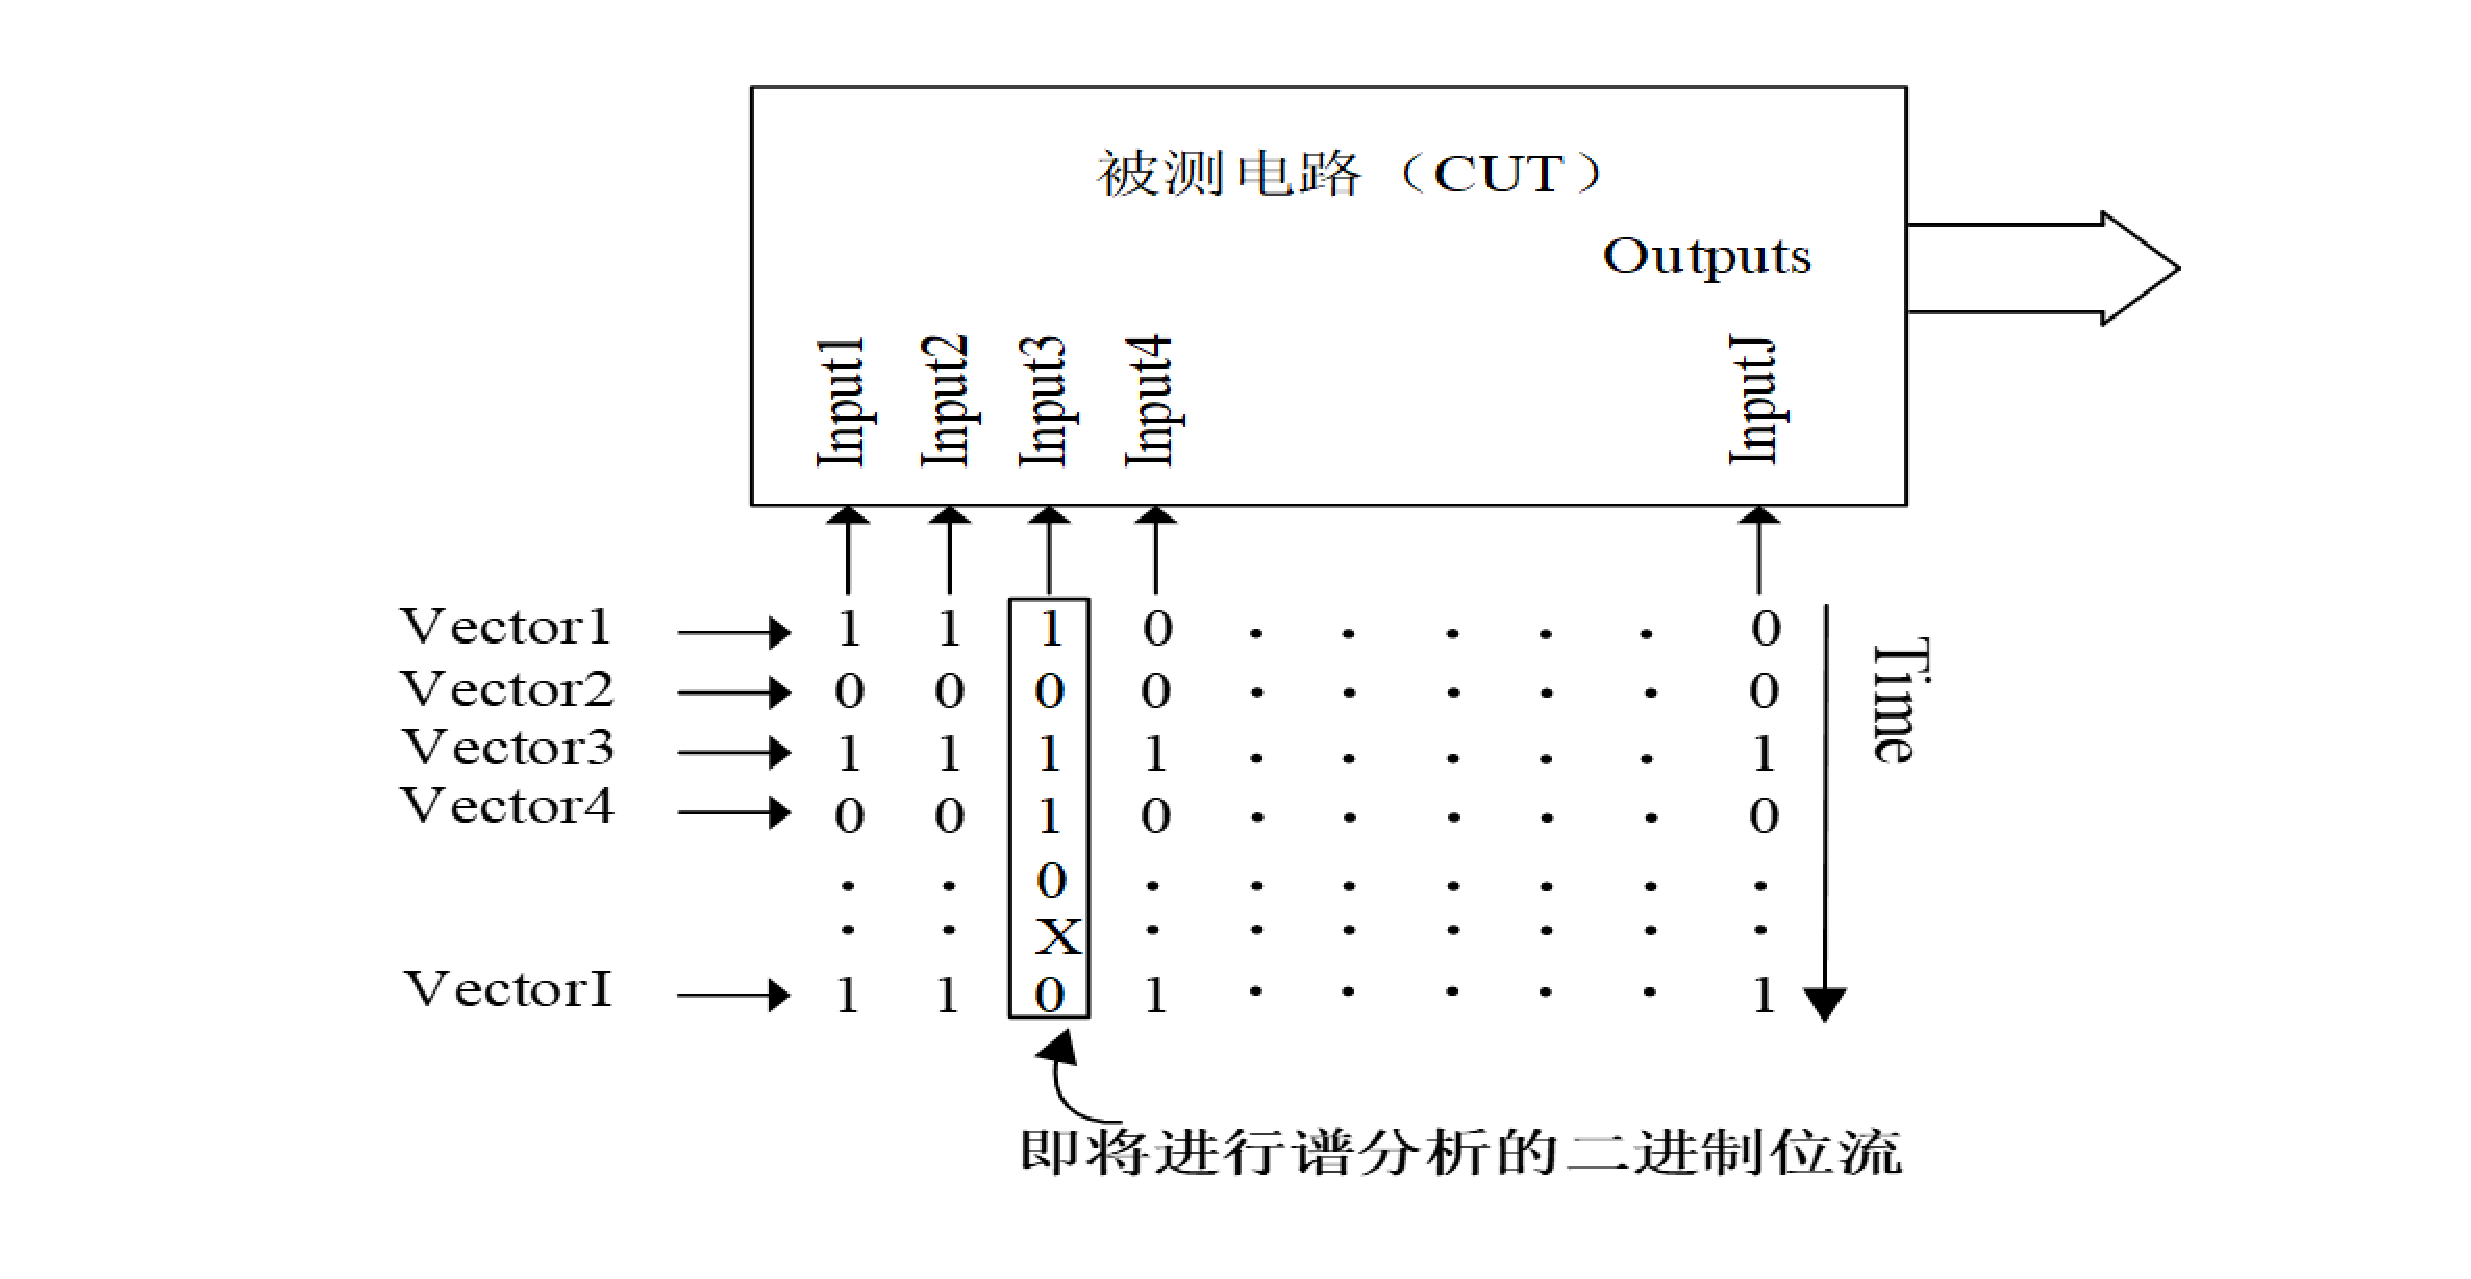
\includegraphics[height=10cm,width=16cm,angle=0,scale=1]{31.eps}
  \caption{测试立方和位流}\label{31}
     \end{figure}

向量分解的伪代码如下算法3.1所示,向量分解是为了提高残差集中0比特位的个数,对于单游程编码而言直接将无关位填充为0即可,拆分压缩技术对于双游程编码的压缩率提升较少,因为影响双游程编码压缩率的关键因素是跳变数,单纯地增加残分量集中的0也不一定会提高最终的压缩率。

\vspace{\baselineskip}
\begin{algorithm}[!h]
	\caption{向量分解}%算法标题
	\begin{algorithmic}%一行一个标行号
        \STATE $N:$ $Number$ $of$ $vectors$
		\STATE $M:$ $Number$ $of$ $inputs$
        \STATE $L:$ $LFSR$ $Matrix$
        \STATE $T[1:N, 1:M]:$ $Test$ $set$ $of$ $dimensions$ $N*M$
        \STATE $Initialization( T )$     // 预处理测试集合
		\FOR{$i=1$ to $M$}
        \STATE $p$ = $L*T[1:N, i]$      //测试集中每一列与位流相乘生成系数矩阵
        \STATE $k$ = $max( p )$         //在系数矩阵p中获取对应下表索引k
		\ENDFOR
		\STATE $Prominent$ = $L[k]$ //生成主分量
        \STATE $Residual$ = $T[1:N, i]$ $XOR$ $Prominent$   //获取残分量集
        \STATE $ProminentComponentSet.add(Prominent)$
        \STATE $ResidualComponentSet.add(Residual)$
        \STATE $Return ProminentComponentSet, ResidualComponentSet$  //返回所需数据
	\end{algorithmic}
\end{algorithm}

如矩阵3.1所示,将列向量(1, 0, 1, 1, 1, X, 0)谱分析后,向量转换为(1, -1, 1, 1, -1, 0, -1)。然后通过线性反馈移位寄存器变换,得到[2 -2 0 0 0 0 -2 5] 这个系数向量。系数向量中系数最大值对应的列向量就是所需的主分量,对应于上图的(1,-1,1,1,1,-1,-1),当系数向量中的最大值有多个时,可以任选其中的任一列作为所求的主分量。在本例中如果将原测试集的无关位填充为0,原列向量与主分量两两异或后最终所得的残差为(0,0,0,0,0,0,0),对于单游程编码,会产生极高的压缩率。若原测试集的列向量长度和线性反馈移位寄存器的矩阵行数不一致,则需要在位流尾部填充无关位或者截断基向量即可。

\begin{equation}
\left[
\begin{array}{ccccccc}
   1& -1& 1& 1& 1& 0& -1\\
\end{array}
\right]
=
\left[
\begin{array}{cccccccc}
    1&   1&   1&-1&   1&-1&-1&   1\\
    1&   1&-1&   1&   1&-1&   1&-1\\
    1&-1&-1&-1&   1&   1&   1&   1\\
    1&-1&   1&   1&-1&-1&   1&   1\\
    1&   1&-1&   1&-1&   1&-1&   1\\
    1&-1&   1&   1&   1&   1&-1&-1\\
    1&   1&   1&-1&-1&   1&   1&-1\\
\end{array}
\right]
\left[
\begin{array}{cccccccc}
   2& -2& 0& 0& 0& 0& -2& 5\\
\end{array}
\right]
\end{equation}

\section{预填充测试集}

\subsection{直接填充与策略填充}

如果采用编码压缩的方式对测试集进行压缩,一旦编码方式得以确定,无关位具体是填充0或者1也随之确定。直接填充就是将不确定位直接填充成为码字0 或者码字1,策略填充就是根据一定的策略进行填充,使得测试集在当前编码规则下的压缩率更高。填充完毕之后,当前的测试集中就不存在无关位,对于一个完全确定的测试集,可以选取合适的聚类算法来选取基向量,最后生成主分量集。本章依旧使用拆分压缩,当无关位填充之后,采取距离最大原则选取基向量生成主分量集。

在以往的研究过程中,并没有采取预填充的手段。对于主分量的选取,有的研究人员采用哈达码变换,有的采取最大相容类变换。通过哈达码变换可以取得较好的压缩增益,但是由于变换产生的列向量与原测试集无关,其获取的压缩率还有提升的空间。而采用最大相容类方式获取的压缩率并不高,由于使用KM算法或者贪婪算法结合关系矩阵法选取基向量,往往因为存在较多无关位,导致算法的时间复杂度过高。采用最大相容类方式确定的第一个基向量能与很多列向量相容,但继续往后选取,与其相容的会越来越少。基向量只能涵盖少数几列测试列向量,只有通过基向量之间两两异或扩展出的其他列向量与原测试中向量越相似,压缩效果才会越好。

\begin{equation}
A
=
\left[
\begin{array}{ccccccccc}
    X&   X&   1&X&   X&X&0&0&0\\
    0&   0&X&   X&   X&1&   1&X&X\\
   1&   0&0&   X&   X&X&   1&1&X\\
   1&   0&X&   X&   X&1&   1&X&X\\
   1&   1&X&   X&   X&X&   1&0&1\\
\end{array}
\right]
\end{equation}

通过一个例子来说明预填充方式的相关做法。上图给出原测试集,分别使用直接填充与策略填充的方式去除测试集中的无关位。下图1 是直接填充方式取得的测试集,采取的是0 填充的方式,如果采取1填充,则将无关为全部填充为1即可。

\begin{equation}
A
=
\left[
\begin{array}{ccccccccc}
    0&0&1&0&0&0&0&0&0\\
    0&0&0&0&0&1&1&0&0\\
    1&0&0&0&0&0&1&1&0\\
    1&0&0&0&0&1&1&0&0\\
    1&1&0&0&0&0&1&0&1\\
\end{array}
\right]
\end{equation}

如若采取策略填充,则需要选择一个默认的编码格式,本例采用FDR编码,直接将无关位填充为0即可,如上所示。如果采用双游程编码,要以原测试集的跳变数最少为原则对无关位进行填充,以EFDR编码为例,填充之后的测试集如下所示:

\begin{equation}
A
=
\left[
\begin{array}{ccccccccc}
   1&1&1&0&0&0&0&0&0\\
   0&0&0&0&0&1&1&1&1\\
   1&0&0&1&1&1&1&1&1\\
   1&0&1&1&1&1&1&1&1\\
   1&1&1&1&1&1&1&0&1\\
\end{array}
\right]
\end{equation}
游程编码不仅要保证跳变数最少,还需要权衡连续出现0或者1的个数,比如跳变数均为2,向量11XXXXXXXXXXXXX000总共有18位,此向量有多种填充方式,一种是将无关位全部填充0,一种是将无关位填充为1,本例应该采取全0方式填充,因为连续的确定位越多获得的压缩效果会越好。

\subsection{选取基向量}

基向量的选取方式至关重要,主分量集是由基向量集合确定的。若基向量集取自原测试集,由基向量集所产生的主分量集与原测试集中的向量相似度会更高,从而增加残差集中0的个数。在本文的第四章中使用聚类算法选取基向量,旨在使选出的基向量尽可能与原测试中的向量相似。为了更好地匹配原测试中已有的列向量,本文在原有的聚类算法上也做了相应的优化。

本章提取基向量的策略分三步进行,第一步随机从原测试集中选取一个列向量当作初始基向量$a$。第二步计算向量$a$与原测试集的每一列向量之间的欧几里得距离$dis$。$dis=\sqrt{((x_1-a_1)^2+(x_2-a_2)^2+....+(x_i-a_i)^2)}$,其中$x$为某一个基向量,$a$ 为原测试集中的某一个列向量,下标即为对应的位,取其中最大的$dis$对应的列向量作为新的基向量。第三步,根据当前确定的基向量求出全部初始基向量,后续步骤$dis$的计算方式为:
\begin{equation}\label{emd}
\centering
      dis=\min⁡(\sqrt{(x_1-a_1)^2+....+(x_i-a_i)^2},....,\sqrt{(y_1-a_1)^2+....+(y_i-a_i)^2)}
               \end{equation}

当有多列基向量时,$dis$为当前列向量与众多基向量两两之间求的欧几里得距离的最小值。对于不同的电路,选取基向量的个数也是不一样的,在本章中基向量选取的个数$X$计算的方式为$X\ge ceil(\log_2^n⁡)$,其中$n$代表当前测试集的行数,由于需要将$X$ 列基向量存储在被测电路中,因此$X$不能取过大,取的过大会浪费存储空间。$X$个列向量之间两两异或将产生$2^X-1$个列向量,主分量集就是由些列向量确定的。上文提及的哈达码矩阵,在拆分压缩中取得了较好的压缩率,$n$ 阶哈达码矩阵有$2^n$行、$2^n$ 列,其中$n$ 的值就是上述$x$ 的值,为了保证自变量一致,本文按照哈达码矩阵变换的规则选取基向量个数。

\section{实验结果与分析}

为了体现预填充方法的可行性,本文对 ISCAS’89\cite{71}中大部分电路进行了验证,包括S5378、S9234、S13207、S15850、S38417、S38584 等电路,本章将挑选其中部分电路做具体分析,计算出其在FDR、EFDR、Huffman 等编码方式下对应的压缩率,并与哈达码变换方法、极大相容类方法进行对比。

本文选取基向量的个数为$X\ge ceil(\log_2^n⁡)$ ,对于$X$列的基向量,两两异或最终可得$2^x-1$个列向量(集合$Y$)。从原测试集中选出每一列,然后将其与集合$Y$中的列向量一一对比,选取出最相似的一列并构造出一个新的集合,即主分量集。实验结果如下表\ref{mtabl1} 所示,首列为电路名称,第二列为当前电路的行数和列数,第三列是变换矩阵的个数,也就是$x$个列向量最终产生向量数的总和,第四列和第五列代表残差集所能达到的最小压缩率和最大压缩率。

\begin{table}[H]
\centering
\caption{随机矩阵与测试集变换结果}\label{mtabl1}
\begin{tabular}{p{2.2cm}p{2.7cm}<{\centering}p{3.3cm}<{\centering}p{2.7cm}<{\centering}p{2.7cm}<{\centering}}
\toprule
\textbf{电路名}&	\textbf{规模}&     \textbf{变换矩阵个数}&   \textbf{最小压缩率}&   \textbf{最大压缩率}\\
\midrule
s5378& (111,214)& 127& 59.64\%& 70.78\%\\
s9234& (159,247)& 255& 58.89\%& 70.12\%\\
s13207& (236,700)& 255& 72.17\%& 93.74\%\\
s15850& (126,611)& 127& 68.14\%& 83.30\%\\
s38417& (99,1664)& 127& 63.03\%& 75.74\%\\
s38584& (126,611)& 127& 68.14\%& 83.30\%\\
平均&        &      &   66.09\%& 78.05\%\\
\bottomrule
\end{tabular}
\end{table}

为了验证本实验是否对多种编码方式均适用,本文选取了FDR、EFDR、ALT-FDR以及Golomb等多种编码方式对变换拆分之后的残差集进行压缩,同时与使用哈达码变换达进行对比。本实验使用了直接填充与策略填充两种方式,直接填充1的效果相对较策略填充和全0填充效果差,策略填充和直接填充0作比较,直接填充0的效果甚至更好,因此为了最大化压缩率本文直接将无关位填充为0。

对于直接将无关位填充为0可以取得最佳的压缩率,猜想如下,第一:拆分压缩的目的是使得残差集中的0 更多,如果直接将无关位填充位0,可以增加残差集中0 的个数。第二:在选取基向量的过程中本文使用基向量之间两两距离最大的原则选取,增加了基向量异或之后所产生向量的多样性,从而获得了更多与原测试集中相似的向量,提高了压缩率。

下表\ref{mtabl2}-\ref{mtabl6}为本方法与哈达码变换以及最大相容类的压缩率对比情况,第一列代表电路名,第二列表示对电路直接使用编码压缩能取得的压缩率,第三列表示对原电路使用哈达码矩阵拆分压缩之后达到的压缩率,第四列为使用最大相容类提取主分量集所获取的压缩率,第五列为使用本方法所能达到的压缩率。以压缩率的提升为原则,本实验直接将无关位填充为0。

表\ref{mtabl2}为FDR编码下各电路的压缩率,电路s13207在不使用拆分压缩的方法下能取得80\%的压缩率,可以说明当前电路所包含的无关位较多。从表中数据可得,直接编码所获取的压缩率普遍较低,使用哈达码变换、最大相容类以及本章方法均可较为明显地提高压缩率。除了s38584 电路,使用预填充的方法所取得的压缩率均高于其他方法,因此取得了最高的平均压缩率。

\begin{table}[H]
\centering
\caption{FDR编码压缩率(\%)}\label{mtabl2}
\begin{tabular}{p{2.2cm}p{2.7cm}<{\centering}p{3.3cm}<{\centering}p{2.7cm}<{\centering}p{2.7cm}<{\centering}}
\toprule
\textbf{电路}&	\textbf{直接编码}& \textbf{哈达码变换}& \textbf{最大相容}& \textbf{本方法}\\
\midrule
s5378&	47.98&	67.51&	67.86&	68.43\\
s9234&	43.61&	66.19&	65.71&	66.39\\
s13207&	81.31&	89.65&	89.92&	91.69\\
s15850&	66.21&	80.66&	80.73&	81.88\\
s38417&	43.27&	72.44&	72.84&	73.04\\
s38584&	60.93&	75.99&	75.34&	75.09\\
平均&	57.22&	75.41&	75.35&	76.08\\
\bottomrule
\end{tabular}
\end{table}

以下是EFDR编码和VIHC编码所对应的压缩率,采用本方法所达到的平均压缩率比哈达码变换高0.79\%,比最大相容类高0.73\%,因此本方法不仅对单游程编码有效,也同样适用于其他编码方式。

\begin{table}[H]
\centering
\caption{EFDR编码压缩率(\%)}\label{mtabl3}
\begin{tabular}{p{2.2cm}p{2.7cm}<{\centering}p{3.3cm}<{\centering}p{2.7cm}<{\centering}p{2.7cm}<{\centering}}
\toprule
\textbf{电路}&	\textbf{直接编码}& \textbf{哈达码变换}& \textbf{最大相容}& \textbf{本方法}\\
\midrule
s5378&	53.67&	64.50&	64.52&	65.60\\
s9234&	48.66&	62.74&	62.62&	62.71\\
s13207&	82.49&	88.89&	88.03&	90.95\\
s15850&	68.66&	78.67&	78.83&	78.88\\
s38417&	62.02&	71.63&	71.76&	71.71\\
s38584&	64.28&	73.45&	72.37&	74.69\\
平均&	63.30&	73.30&	73.36&	74.09\\
\bottomrule
\end{tabular}
\end{table}

\begin{table}[H]
\centering
\caption{VIHC编码压缩率(\%)}\label{mtabl4}
\begin{tabular}{p{2.2cm}p{2.7cm}<{\centering}p{3.3cm}<{\centering}p{2.7cm}<{\centering}p{2.7cm}<{\centering}}
\toprule
\textbf{电路}&	\textbf{直接编码}& \textbf{哈达码变换}& \textbf{最大相容}& \textbf{本方法}\\
\midrule
s5378&	51.75&	69.63&	69.66&	70.78\\
s9234&	47.23&	69.58&	69.53&	70.12\\
s13207&	83.55&	92.20&	91.91&	93.74\\
s15850&	67.97&	82.96&	82.98&	83.30\\
s38417&	53.39&	74.79&	74.83&	75.74\\
s38584&	62.30&	78.11&	78.80&	79.50\\
平均&	61.03&	77.89&	77.83&	78.86\\
\bottomrule
\end{tabular}
\end{table}

\begin{table}[H]
\centering
\caption{RL-Huff编码压缩率(\%)}\label{mtabl5}
\begin{tabular}{p{2.2cm}p{2.7cm}<{\centering}p{3.3cm}<{\centering}p{2.7cm}<{\centering}p{2.7cm}<{\centering}}
\toprule
\textbf{电路}&	\textbf{直接编码}& \textbf{哈达码变换}& \textbf{最大相容}& \textbf{本方法}\\
\midrule
s5378&	52.58&	64.02&	64.14&	66.73\\
s9234&	47.26&	60.33&	60.16&	63.16\\
s13207&	82.49&	88.71&	88.81&	92.23\\
s15850&	67.35&	77.33&	77.99&	79.47\\
s38417&	63.32&	69.66&	69.64&	71.43\\
s38584&	62.40&	71.05&	72.28&	72.91\\
平均&	62.57&	71.85&	72.17&	74.32\\
\bottomrule
\end{tabular}
\end{table}

\begin{table}[H]
\centering
\caption{ALT-FDR编码压缩率(\%)}\label{mtabl6}
\begin{tabular}{p{2.2cm}p{2.7cm}<{\centering}p{3.3cm}<{\centering}p{2.7cm}<{\centering}p{2.7cm}<{\centering}}
\toprule
\textbf{电路}&	\textbf{直接编码}& \textbf{哈达码变换}& \textbf{最大相容}& \textbf{本方法}\\
\midrule
s5378&	49.95&	61.62&	62.02&	63.54\\
s9234&	44.96&	58.31&	58.16&	58.89\\
s13207&	80.23&	86.52&	86.61&	90.16\\
s15850&	65.83&	75.76&	75.89&	76.78\\
s38417&	60.55&	68.40&	67.51&	68.13\\
s38584&	61.13&	69.70&	71.83&	72.09\\
平均&	60.58&	70.06&	70.24&	71.60\\
\bottomrule
\end{tabular}
\end{table}

AFER和RL-Huff编码均是双游程编码,由上图可以得RL-Huff编码和ALT-FDR编码比哈达码变换所取得的压缩率平均高出2.47\%和1.54\%,比最大相容所取得的压缩率高2.15\%和1.36\%。

从表\ref{mtabl2}-\ref{mtabl6}中的结果可知,本方法与直接编码、哈达码变换以及最大相容类三种方法对比,均取得了较高的压缩率。

表\ref{mtabl7}中的数据为本方法与其他压缩方法在不同电路下获取的压缩增益,本方法的压缩率为使用FDR 编码所达,SVC 使用的是对称编码。L-EFDR 属于双游程编码,对EFDR 编码进行了改进,提高了压缩率。LHBE 方法先对确定位进行划分,再进行编码,降低了编码的比特数量。由实验结果可知,本方法的平均压缩率高达76.28\%,与其他压缩方法相比较均有提高。结果表明对无关位预填充,同时在选取基向量时,按照距离跨度最大的方式选取可以获取较高的压缩增益。从表中数据分析可知,不管使用何种压缩方法,s13207所取得的压缩率均是最高的,由此推断s13207电路中无关位会比较多。通过观察其测试集,也验证了这一推论。

\begin{table}[H]
\centering
\caption{本方法与其他压缩方法压缩率比较(\%)}\label{mtabl7}
\begin{tabular}{p{1.6cm}p{2.36cm}<{\centering}p{2.36cm}<{\centering}p{2.36cm}<{\centering}p{2.36cm}<{\centering}
p{2.36cm}<{\centering}}
\toprule
\textbf{电路名}&	\textbf{SVC\cite{72}	}& \textbf{I-EFDR\cite{73}}& \textbf{LHBE\cite{74}}& \textbf{CCPRL\cite{75}}& \textbf{本方法}\\
\midrule
s5378&	51.80&	55.10&	53.10&	61.08&	68.43\\
s9234& 	50.94& 	52.73& 	52.33& 	62.95&	66.39\\
s13207& 83.77& 	83.82& 	83.87& 	90.06& 	91.69\\
s15850& 69.98& 	71.05& 	70.78& 	76.32& 	80.88\\
s38417& 63.30& 	64.57& 	64.10& 	64.61& 	73.04\\
s38584& 66.26& 	66.70& 	66.60&	75.38& 	77.06\\
平均& 	64.34& 	68.01& 	65.13& 	71.73& 	76.28\\
\bottomrule
\end{tabular}
\end{table}

\section{小结}

为了降低电路的存储开销,提高数据压缩率,本章基于变换压缩的研究方法提出了一种预填充方法,此方法预先对测试集进行处理,去除原测试集中的无关位。此方法有直接填充与策略填充两种模式,对于拆分压缩直接将无关位填充为0效果最佳。其次,在基向量的选取过程中并不是一味随机选取,而是随机选取第一列,然后根据欧几里得距离依次确定其他的基向量,基向量两两之间差距的增大导致异或之后产生的列向量更加丰富,从而提高了压缩率。实验结果表明,使用本方法可以大大提高压缩率并减少了测试集的存储代价,节约测试时间成本。

% !Mode:: "TeX:UTF-8"

\chapter{使用聚类算法提高压缩率}

聚类算法是器学习中的一类经典算法,常用于数据分类与数据特征提取,聚类即物以类聚,通过定义了一个分类标准,对原数据集进行划分。机器学习中涉及的算法众多,总体可分为基于监督学习与非监督学习两类,聚类算法初始并无任何标记,也无特征可以提取,对于不同的数据集,其采取的距离计算方式也是不一样的,因此被归于无监督学习一类。无监督学习的算法需要自动找到这些无标记数据集所具有的特征。

本文将聚类算法与数据压缩相结合,通过对原测试集进行分析,提取其中的特征,找到了一种提高压缩率的方法。在本文第三章使用预填充测试集结合距离优先法则选取了基向量,最终获得了较好的压缩增益,但是基向量的选取是毫无规律的,具有较大的随机性,如果使用聚类算法,对原测试集进行聚类,以聚类中心作为基向量生成主分量集,在一定程度上能增大与原测试集的相似程度,理论上来说可进一步提高残差集的压缩率。

\section{kmeans聚类算法}

Kmeans算法又叫做k-平均算法(英文:k-means clustering),是集简单和经典于一身的以距离作为考量标准的聚类算法。kmeans算法将距离相近的点归结于同一类,一般而言可以使用欧几里得距离、曼哈顿距离或者海明距离等作为“距离”的考量标准。kmeans算法是一种比较经典的聚类算法,其实现简单聚类效果较好,但是初始聚类中心的选取对结果的影响较大,往往需要通过一些特定的优化手段或者限定条件使其获得稳定而可靠的实验结果。

不同的聚类算法之间的聚类原理不同,约束条件也不一样,最终的聚类结果也不一样。当选取某个聚类算法时需要结合自身的使用场景,具体问题具体分析。有些聚类算法需要事先给定聚类个数,无法简单地通过迭代直接确定数据集的特征自动划分聚类数,比如kmeans 和kmeans++ 算法。有些聚类算法需要实现给定"密度",比如dbscan聚类算法,虽然此方法可对数据集自动聚类但在算法运行的开始需要给定密度的具体值。其对$n$个样本点属于同一聚类的定义为,若样本中心在以$d$为半径的区域类有$n$个样本点,则这些样本可以划分为同样一类。因此聚类算法的运用是十分灵活的,如何更好的结合自身往往需要对不同聚类算法进行大量的实验,分析其中的原理。分类算法也可以用于数据的划分,但是不适合本实验,聚类与分类算法的最大区别在于,分类的目标类别已知,而聚类的目标类别是未知的。下文将着重介绍kmeans聚类算法,首先简要了解kmeans算法的相关术语

簇:所有数据的点集合,簇中的对象是相似的。

质心:通过计算所有点的均值得到簇的质心。

SSE:Sum of Sqared Error(误差平方和), 它被用来评估模型的好坏,SSE 值越小,表示越接近它们的质心. 聚类效果越好。由于对误差取了平方,因此更加注重那些远离中心的点(一般为边界点或离群点)。

\begin{figure}[H]
  \centering
  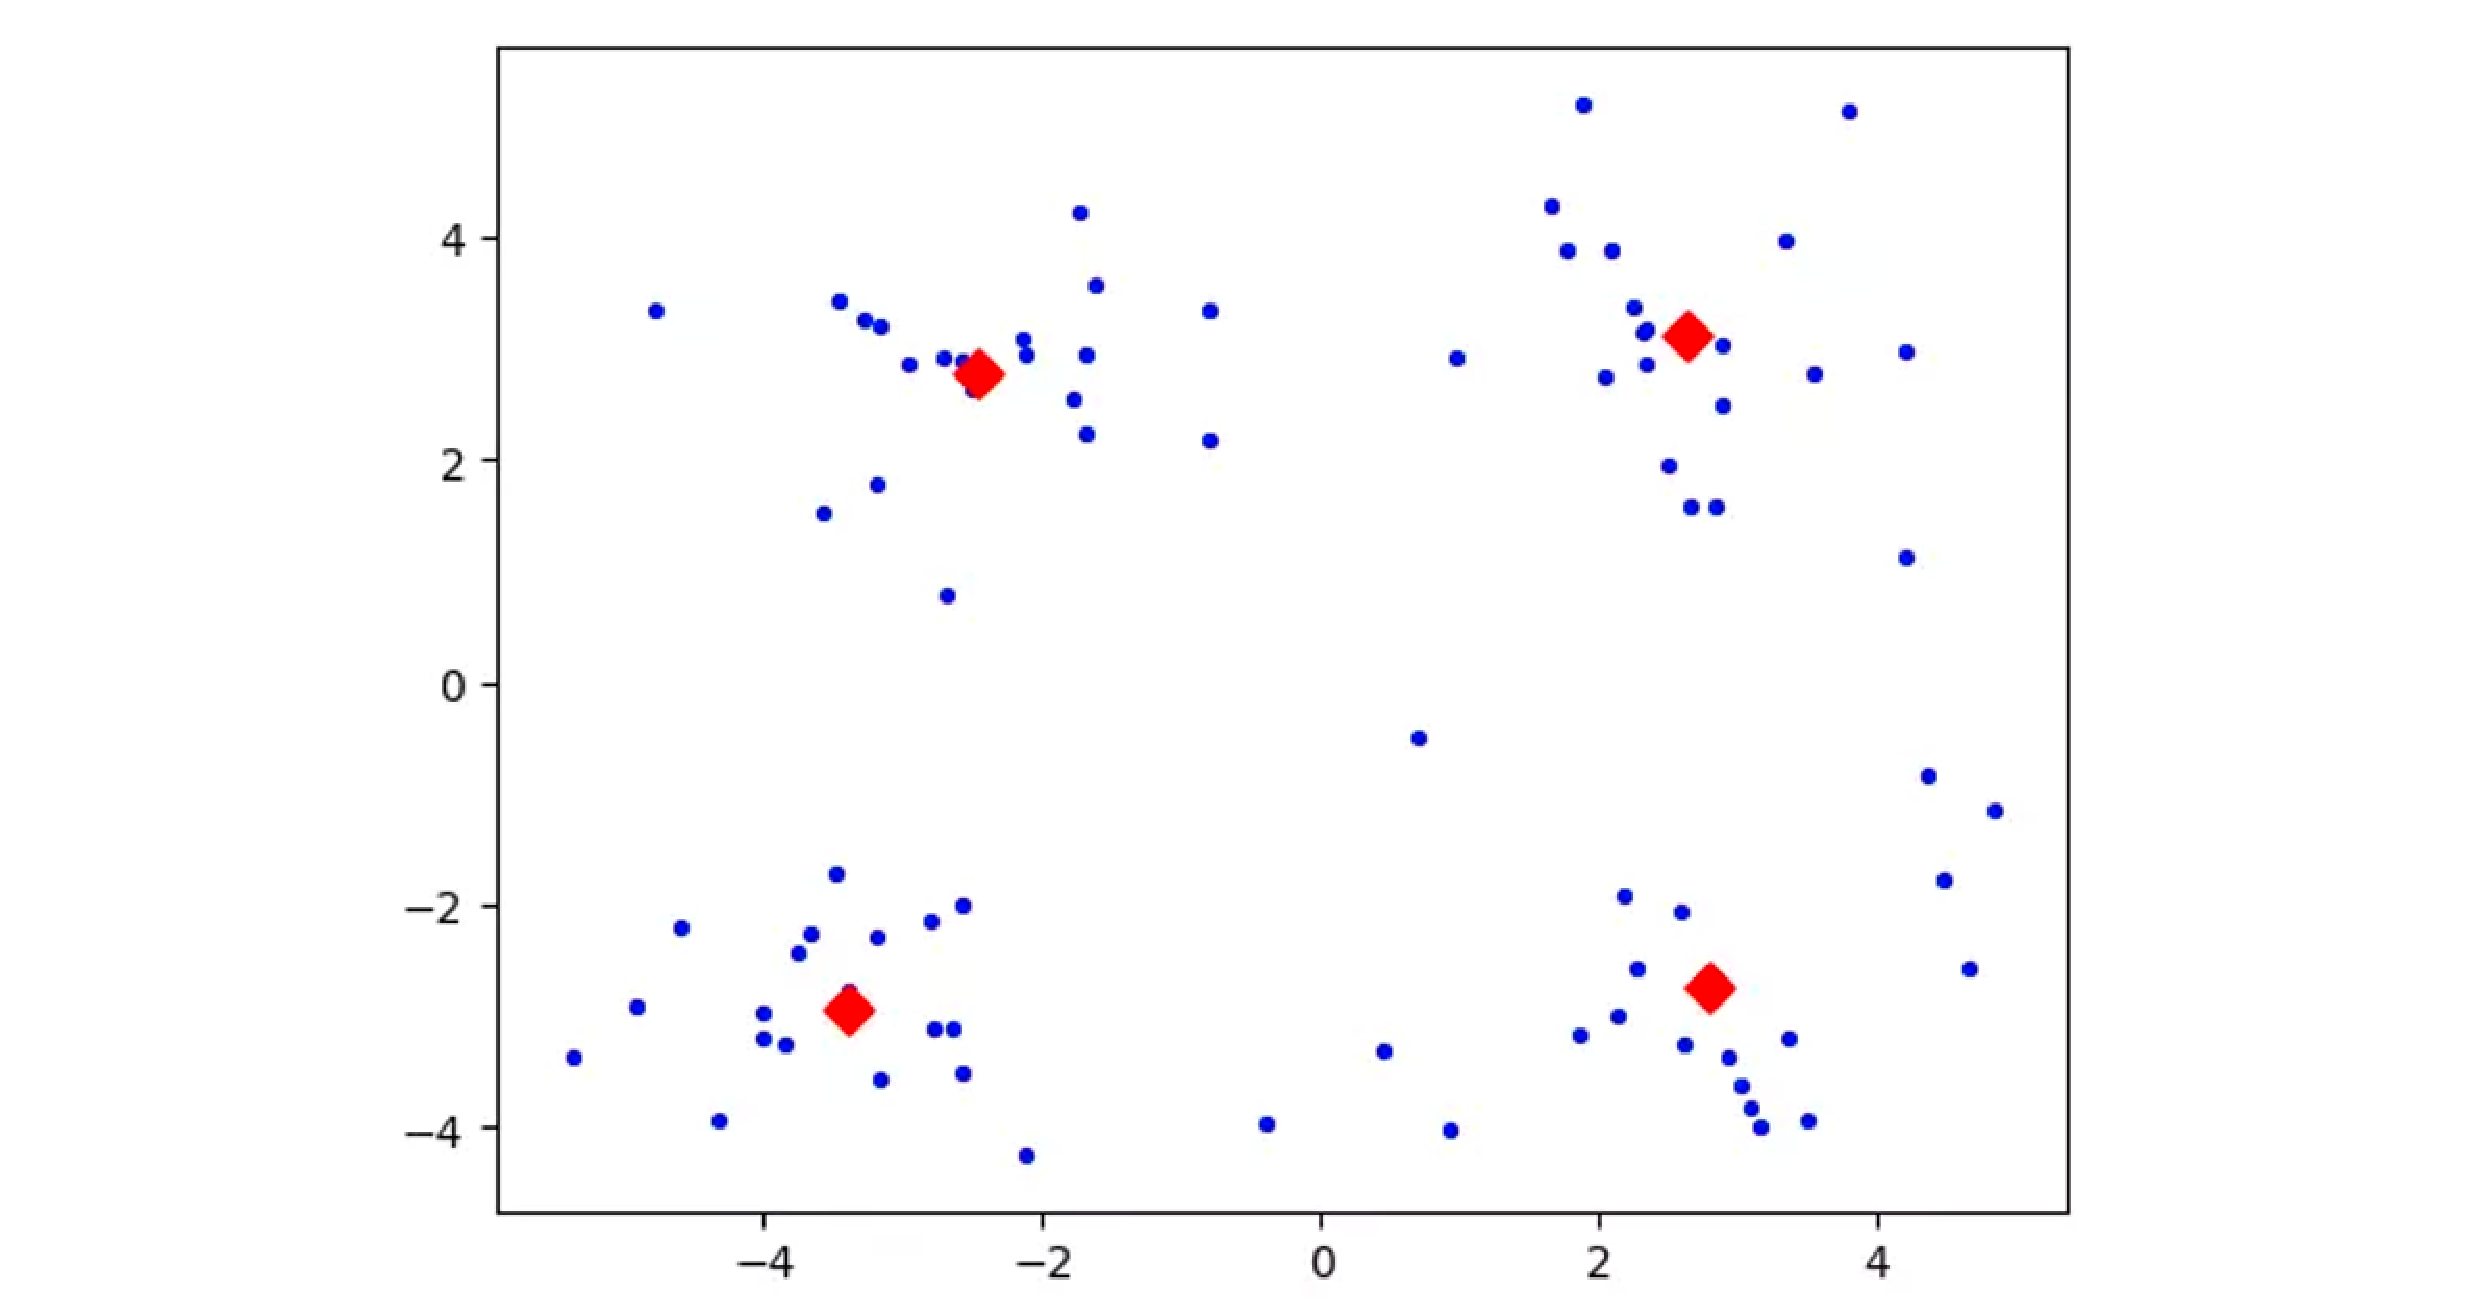
\includegraphics[height=8cm,width=16cm,angle=0,scale=1]{42.eps}
  \caption{聚类分布状态图}\label{42}
     \end{figure}

从上图\ref{42}中的数据分布可以看出,样本点大致分为四簇。所以设置初始聚类中心 $k=4$,如果对数据不是很了解,可以先设置一个$k$,进行聚类之后,再根据结果的聚类效果来调整聚类中心的数量。上图可以看成二维坐标,其中每一个点都有相对应的x坐标和y坐标,通过欧几里得距离公式计算出SSE。Kmeans算法的计算流程如下所示:

(1)首先确定一个$k$值,即我们希望将数据集经过聚类得到$k$个集合。一般而言$k$值并不是事先所知晓的需要尝试多次。

(2)从原数据集合中随机确定$k$个点作为聚类中心。

(3)对数据集中每一个点,计算其与每一个质心的距离(如欧式距离),离哪个质心近,就划分到那个质心所属的集合。

(4)把所有数据归好集合后,一共有$k$个集合。然后重新计算每个集合的质心。

(5)重复步骤3至步骤5,直到集合之间质心间的距离差低于某个阈值算法迭代结束。

通过上述的步骤基本上可以将一组数据划分成为$k$个聚类,本文将其转化为数学表达式,假设簇划分为 $(C_1,C_2,C_3,....,C_N)$, 则本实验的目标是最小化平方误差E:

\begin{equation}\label{emd}
\centering
      E=\sum_{i=1}^n\sum_{x\in C_i}^n||x-u_i||_2^2
               \end{equation}

其中$u_i$为$C_i$的均值向量其表达式为:

\begin{equation}\label{emd}
\centering
     u_i=\frac{1}{\ |C_i|}\sum_{x\in C_i}^{ }x
               \end{equation}

为了进一步理解kmeans算法,本章以二维坐标系为例,讲述如何划分聚类。在二维坐标系中有6个点分别为$p1(0,0),p2(1,2 ),p3(3,1),p4(8,8),p5(9,10),p6(10,7)$,点与点之间的距离直接使用欧几里得距离公式计算,如果点并不是二维的坐标轴上,而是在三维、四维甚至$n$维,其距离计算公式为对应位两两相减求平方和之后开更根号。由于数据量较小,通过观察可得本数据可以划分为两个聚类,为了演示效果直接令$k=2$。初始时随机选两个点$p1$和$p2$,计算出剩余点与其距离如下表\ref{ptabl1}所示:

\begin{table}[H]
\centering
\caption{测试集的划分和各种块出现的频率}\label{ptabl1}
\begin{tabular}{p{4cm}<{\centering}p{4cm}<{\centering}p{4cm}<{\centering}}
\toprule
\textbf{坐标点}&	\textbf{P1}&     \textbf{P2}\\
\midrule
P3	&3.16	&2.24\\
P4	&11.3	&9.22\\
P5	&13.5	&11.3\\
P6	&12.3	&10.3\\
\bottomrule
\end{tabular}
\end{table}


按照距离为原则划分两组中的数据为:组A中只有$p1$,组B中为其他点。
第二步分别计算A组和B组的质心,A组质心为$p1=(0,0)$,B组质心为$pB=(6.2,5.6)$,质心的计算公式为簇中各个向量相加取平均值即可。第三步,以质心为原点计算每一个点到质心的距离再次分组距离分布如下表\ref{ptabl2}所示:

\begin{table}[H]
\centering
\caption{测试集的划分和各种块出现的频率)}\label{ptabl2}
\begin{tabular}{p{4cm}<{\centering}p{4cm}<{\centering}p{4cm}<{\centering}}
\toprule
\textbf{坐标点}&	\textbf{P1}&     \textbf{P2}\\
\midrule
P2	&2.24	&6.3246\\
P3	&3.16	&5.6036\\
P4	&11.3	&3\\
P5	&13.5	&5.2154\\
P6	&12.2	&4.0497\\
\bottomrule
\end{tabular}
\end{table}

第二次分组结果为组$A$:$p1$、$p2$、$p3$。组$B$:$p4$、$p5$、$p6$。再次计算质心轮询上面的步骤直至组A和组B中的点不发生变化,迭代结束。根据上述实验思路给出具体的算法流程伪代码如下所示:

\begin{algorithm}[!h]
	\caption{Kmeans}%算法标题
	\begin{algorithmic}%一行一个标行号
        \STATE 输入$:$   $ $类簇个数K,迭代终止阈值$\phi$,最大迭代次数$MAX\_COUNT$
        \STATE 输出$:$   $ $聚类结果
        \FOR{$k=0$ to $K$}
        \STATE $center_k$ = $rand()\%COUNT$ //初始化K个类簇的聚类中心
        \ENDFOR
        \FOR{$k=0$ to $MAX\_COUNT$}
        \FOR{$t=0$ to $T$}
        \STATE $For$ $every$ $x_i$ //所有数据对象
        \STATE $Dis(x_i,center_k)$ //将$x_i$归于某一个聚簇中
        \ENDFOR
		\FOR{$k=0$ to $K$}
        \STATE $center_k=avg(cluster(k))$ // 将每一个聚簇的平均值作为新的聚类中心
        \ENDFOR
        \STATE $Diff$ = $new(cluster)-old(cluster)$
        \IF{$Diff <=\phi$}
		\STATE $return$  $res$ // 如果新旧聚簇无明显变化则终止循环
		\ENDIF
        \ENDFOR
        \STATE $return$  $res$
	\end{algorithmic}
\end{algorithm}

Kmeans算法其优势是简单且易于实现,收敛速度快,对于结果密集型且区别明显的聚类簇分类效果好,但是其缺陷也非常明显,首先我们需要手动确定聚类数$K$,若原数据集并不能直接分为$k$个聚类有$2k$或者数据集较为分散没有明显特征,kmeans算法效果就会较差。其次kmeans对初始质心的选取依赖较大,不同的随机种子对结果影响非常明显。

因此有学者提出了kmeans++算法,其改进主要针对kmeans算法会随机选取初始质心。kmeans++在质心选取之前还进行了几个步骤,第一步从原数据集合中任意挑选出一个数据作为初始聚类中心。第二步,计算出集合中其他数据与初始聚类中心之间的距离,并将其相加,然后取随机值$r$,若$r$等于某一个数据与聚类中心之间的距离则将当前数据设置为新的聚类中心。第三步,重复上述步骤,直到确定所有的聚类中心。本文所使用的的kmeans++算法在第二步与传统做法有所不同,本人的做法为,若原数据集中有$x$个数据点,求出将$x$个数据点与聚类中心之间的欧式距离,选取其中最远的距离对应的数据作为第二个聚类中心,依次迭代获取最终的初始聚类中心。

\section{聚类算法结合测试集选取基向量}

\subsection{聚类算法的选择}

本人使用了多种聚类算法进行相关实验,包括基于密度的dbscan聚类算法、基于机器学习的马尔科夫模型以及基于均值漂移相关的聚类算法。基于密度聚类的算法过于依赖密度的大小,密度又取决于邻域范围的设定以及邻域中列向量个数的设定。实验结果表明kmeans++ 算法能较好地结合原测试集,提高压缩率。dbscan聚类算法虽然可以自动确定聚类个数,但是需要设置$\epsilon$-邻域以及$MinPts$。 本人经过多次尝试发现对于不同的电路,其$\epsilon$-邻域以及$MinPts$均不相同,无法给出统一的标准,而且这两个值需要不断尝试才能获取较好的压缩增益,如果设置不当与随机选取无异。

Kmeans算法主要的缺陷有两点,第一无法确定数据集需要聚类的数目$K$,第二,只能随机选取初始质心。争对这两个缺陷本文给出了解决方案,首先本文根据电路的行来确定需要聚类的数目$K$,这样做有两点好处,第一对于不同的电路都适用,具有通用性。第二,会保证最终的聚类数不会过多,本实验最终要选择聚类中心充当基向量,若聚类数过多会导致基向量过多,增加硬件开销。针对第二个缺陷,本文结合kmeans++的思想,使用一种极大化质心(基向量)距离的选取方式,保证了初始质心(基向量)之间的距离足够远。通过上述两种解决方案,本实验使用kmeans++算法对已填充的原测试进行聚类。下文将介绍详细过程。

\subsection{基向量的选取}

基向量选取完成后,测试集相对应的主分量集也随之确定。本章主要根据kmeans++聚类算法计算出本文所需要的基向量。

在初始基向量的选取过程中,需要进行测试集预填充,由于本人采取拆分压缩的压缩方法,将原测试集中的无关位填充为0即可。本实验所需要的基向量即为将原测试集聚类之后所产生的聚类中心,下面是选取的具体步骤:为了方便表述,将聚类中心使用基向量来表述。

(1)将原测试集进行预填充,并从中任意挑选出一个列向量作为初基向量,由于是随机选取本实验直接使用第一列作为初始基向量。

(2)依次求出原测试集中其他列向量与,已挑选基向量之间的欧式距离,取距离最大的一列作为第二个选取的基向量。

(3)在原测试集中选取其他列向量作为下一个基向量,将其类比为数学公式为$D_x=\max⁡(D_1,D_2,.....,D_N)$,其中$D_1$表示测试集中第一个列向量与基向量之间的最小距离。同理$D_N$表示测试集中第$N$个列向量与基向量之间的最小距离,这个步骤主要保证基向量之间的距离最大。

(4)重复上述步骤直至确定$k$初始基向量,其中$k$的数量由我们原测试集的数据规模决定。

(5)计算出原测试集中每一列与初始基向量之间的距离。

(6)每个列向量均能计算出$k$个距离,$k$个距离就代表$k$聚类,以距离最小为原则将其划分到相应的聚类中。

(7)确定$k$个聚类之后,将每个聚类中的列向量相加之后求平均值,获取新的聚类中心,即新的基向量。

(8)判断新选取的基向量计算的阈值是否小于等于事先给定的阈值,一旦满足迭代终止条件则,当前获取的基向量为本文所求,如果不满足则返回第二步重复计算。迭代条件可以设定为迭代之后类族的中心点不发生变化或者直接初始化迭代的次数。

\vspace{\baselineskip}
\begin{algorithm}[!h]
	\caption{$PrincipalComponentSetGenerationl$ $(T)$}%算法标题
	\begin{algorithmic}%一行一个标行号
        \STATE 输入$:$   $ $初始$K$个基向量
        \STATE 输出$:$   $ $主分量集
        \STATE $N:$ $Number$ $of$ $vectors$
		\STATE $M:$ $Number$ $of$ $columns$
        \STATE $J[1:N,1 ceiling(log2N)]$ : $Base$ $vector$ $matrix$
        \STATE $T[1:N, 1:M]:$ $Test$ $set$ $set$ $size$
        \STATE $Z=Xor(J)$     //将基向量两两间进行异或得到矩阵$Z$
        \STATE $Z=[Z,-Z]$    //将矩阵Z取反与原来的Z组成新矩阵
		\FOR{$i=1$ to $M$}
        \STATE $d$ = $Hamming(Z,T[1:N, i])$     //计算矩阵$Z$与原测试集中第i列的汉明距离
        \STATE $t$ = $min(d)$         $    $  //求出汉明距离$d$中绝对值最小所对应的索引k
        \STATE $Principal$ = $Z[t]$ //提取主分量
        \STATE $PrincipalComponentSet add(Principal)$
		\ENDFOR
        \STATE $Return PrincipalComponentSet$  //返回主分量集
	\end{algorithmic}
\end{algorithm}

\subsection{主分量集的获取}

得到$K$个基向量后,将其两两之间进行异或,可得到一个列向量数为$2^n-1$的矩阵,然后将这个矩阵取反且与原矩阵拼成一个新的矩阵,计算测试集中的列与新矩阵中的每一列的汉明距离,选取汉明距离最小所对应的列作为主分量,构成主分量集,得到主分量集后,将它与原测试集进行异或,生成残分量集,最后对残分量集进一步压缩。主分量生成的具体过程如算法4.2所示。

例如测试集A的基向量为$\beta_1$(1,0,1,0,1)、$\beta_2$(1,1,0,0,1)、$\beta_4$(0,1,1,1,1)组成,通过基向量两两异或可生成矩阵Z,基向量为三列,对应的Z为7列。

\begin{equation}
Z
=
(\beta_1,\beta_2,\beta_4,\beta_1\bigoplus \beta_2,\beta_1\bigoplus \beta_4,\beta_2\bigoplus \beta_4,\beta_1\bigoplus \beta_2\bigoplus \beta_4)
=
\left[
\begin{array}{ccccccc}
    1&1&0&0&1&1&0\\
    0&1&1&1&1&0&0\\
    1&0&1&1&0&1&0\\
    0&0&1&0&1&1&1\\
    1&1&1&0&0&0&1\\
\end{array}
\right]
\end{equation}


然后将Z取反与原矩阵拼接成为全新矩阵 ,取反即为0和1位置互换。

\begin{equation}
Z
=
\left[
\begin{array}{cccccccccccccc}
    1&1&0&0&1&1&0&0&1&1&1&1&0&0\\
    1&0&1&1&0&1&0&0&0&1&0&1&1&1\\
    1&1&1&0&0&0&1&0&0&1&1&0&0&1\\
    1&0&0&0&0&1&1&0&1&0&0&1&0&1\\
    1&1&0&1&0&0&0&0&0&0&1&1&1&0\\
\end{array}
\right]
\end{equation}

最终计算出测试集A中的每一列与矩阵$Z$每一列的汉明距离$dis$,将$dis$所对应 中的列向量作为当前测试集中相应列的主分量。例如测试集中第二列$β2(1,1,0,0,1)$ 与矩阵$Z$中第二列(1,1,0,0,1)的汉明距离为0,则原测试集第二列的主分量为(1,1,0,0,1)。依此类推,直到计算出原测试集每一列所对应的主分量,构造出主分量集。最终将主分量集合原测试集进行异或,计算出相应残差集,获取压缩率。

\section{实验结果与分析}

本实验中选择的kmeans++算法,需要预先设定聚类中心的个数$k$,聚类数$k$定义得过少或者过多对结果均会产生一定的影响。针对此问题,本文分两个步骤进行了相关实验。第一部分根据电路大小选取基向量个数,并取得压缩率,同时与其他拆分压缩所取得的压缩率进行对比。第二部分,由于基向量需要存储代价,基向量的选取不能无限制的增加,本人在一定范围内动态增加或者减少基向量个数,观察压缩率的变化情况,大致绘制出基向量--压缩率之间的趋势变化图。

\subsection{根据电路大小确定基向量数}

根据电路大小选取基向量,其选取方式为$k=ceil(\log_2^N⁡)$其中$N$为测试集的行数。为了验证聚类算法的有效性,本文对S5378、S9234、S13207、S15850、S38417、S38584等电路进行了实验,下文将对其中部分电路做具体描述,同时与其他压缩方式所得的压缩增益做对比。

实验结果如下表\ref{ptabl3}-\ref{ptabl7}所示,本文选取了FDR、EFDR、ALT-FDR、RL-Huff、VIHC以及Golomb六种编码方式对变换拆分之后的残差集进行压缩,同时与使用哈达码变换、直接预填充方式获取的压缩率进行对比。

第一列为电路名称,第二列为测试集直接压缩之后的结果,第三列是对哈达码变换拆分之后的压缩率,第四列为对测试集预填充所获取的压缩率,第五列是由kmeans++聚类算法结合拆分压缩所的压缩率。

表\ref{ptabl3}是 FDR 编码在各种情况下的压缩率比较,FDR 编码是一种单游程编码方式,其对连续0子串进行编码,遇到1比特位直接使用00进行编码,当0串越长所对应的码字相对于原串越短,压缩率越高。由表中的数据可知,采用本章方法计算的压缩率比对测试集直接编码平均高20\%,比哈达码变换平均高2.4\%,比预填充方法平均高1.72\%。

\begin{table}[H]
\centering
\caption{FDR编码压缩率(\%)}\label{ptabl3}
\begin{tabular}{p{2.2cm}p{2.7cm}<{\centering}p{3.3cm}<{\centering}p{2.7cm}<{\centering}p{2.7cm}<{\centering}}
\toprule
\textbf{电路}&	\textbf{直接编码}& \textbf{哈达码变换}& \textbf{预填充}& \textbf{本方法}\\
\midrule
s5378&	47.98&	67.51&	68.43&	70.76\\
s9234&	43.61&	66.19&	66.39&	69.59\\
s13207&	81.31&	89.65&	91.69&	92.29\\
s15850&	66.21&	80.66&	81.88&	81.75\\
s38417&	43.27&	72.44&	73.04&	75.35\\
s38584&	60.93&	75.99&	75.09&	77.03\\
平均&	57.22&	75.41&	76.08&	77.80\\
\bottomrule
\end{tabular}
\end{table}

表\ref{ptabl4}展示了 EFDR 编码在不同压缩方法下所获取压缩增益,EFDR 编码是一种双游程编码方式,属于对 FDR 编码的一种扩展,既可以对0 游程进行编码,也可以对1进行编码,对测试集中0和1的数目并没有具体的要求,只需要保证跳变数最少即可,如果测试集中0 和1 相继出现,压缩效果就会比较差,由表可知,采用本章描述的方法所获取的压缩率比对测试集直接编码获取的压缩率平均高 12.37\%,比哈达码变换获取的压缩率平均高 2.37\%,比在预填充方法下获取的压缩率平均高 1.58\%。

\begin{table}[H]
\centering
\caption{EFDR编码压缩率(\%)}\label{ptabl4}
\begin{tabular}{p{2.2cm}p{2.7cm}<{\centering}p{3.3cm}<{\centering}p{2.7cm}<{\centering}p{2.7cm}<{\centering}}
\toprule
\textbf{电路}&	\textbf{直接编码}& \textbf{哈达码变换}& \textbf{预填充}& \textbf{本方法}\\
\midrule
s5378&	53.67&	64.50&	65.60&	67.75\\
s9234&	48.66&	62.74&	62.71&	66.14\\
s13207&	82.49&	88.89&	90.95&	91.60\\
s15850&	68.66&	78.67&	78.88&	79.84\\
s38417&	62.02&	71.63&	71.71&	74.06\\
s38584&	64.28&	73.45&	74.69&	74.60\\
平均&	63.30&	73.30&	74.09&	75.67\\
\bottomrule
\end{tabular}
\end{table}

表\ref{ptabl5}-\ref{ptabl6}展示了 ALT-FDR 编码和 RL-Huff 编码在不同压缩方法下所获取压缩增益。由表可知,采用本章所提出的方法,ALT-FDR 编码和RL-Huff 编码所获取的压缩率比对测试集直接编码平均高12.42\%和13.73\%,比哈达码变换获取的压缩率平均高 3.24\% 和4.45\%,比预填充策所达到的平均压缩率分别高 1.7\%和 1.98\%。虽然ALT-FDR 编码和 RL-Huff 编码都是属于双游程编码,需要根据跳变数最少来进行编码,但是较其他压缩方法使用本方法获取的压缩增益依然是最高的。

\begin{table}[H]
\centering
\caption{ALT-FDR编码压缩率(\%)}\label{ptabl5}
\begin{tabular}{p{2.2cm}p{2.7cm}<{\centering}p{3.3cm}<{\centering}p{2.7cm}<{\centering}p{2.7cm}<{\centering}}
\toprule
\textbf{电路}&	\textbf{直接编码}& \textbf{哈达码变换}& \textbf{预填充}& \textbf{本方法}\\
\midrule
s5378&	49.95&	61.62&	63.54&	65.17\\
s9234&	44.96&	58.31&	58.89&	62.72\\
s13207&	80.23&	86.52&	90.16&	90.88\\
s15850&	65.83&	75.76&	76.78&	77.82\\
s38417&	60.55&	68.40&	68.13&	71.23\\
s38584&	61.13&	69.70&	72.09&	71.97\\
平均&	60.58&	70.06&	71.60&	73.30\\
\bottomrule
\end{tabular}
\end{table}

\begin{table}[H]
\centering
\caption{RL-Huff编码压缩率(\%)}\label{ptabl6}
\begin{tabular}{p{2.2cm}p{2.7cm}<{\centering}p{3.3cm}<{\centering}p{2.7cm}<{\centering}p{2.7cm}<{\centering}}
\toprule
\textbf{电路}&	\textbf{直接编码}& \textbf{哈达码变换}& \textbf{预填充}& \textbf{本方法}\\
\midrule
s5378&	52.58&	64.02&	66.73&	68.59\\
s9234&	47.26&	60.33&	63.16&	67.07\\
s13207&	82.49&	88.71&	92.23&	92.82\\
s15850&	67.35&	77.33&	79.47&	80.57\\
s38417&	63.32&	69.66&	71.43&	74.02\\
s38584&	62.40&	71.05&	72.91&	74.74\\
平均&	62.57&	71.85&	74.32&	76.30\\
\bottomrule
\end{tabular}
\end{table}

表\ref{ptabl7}展示了 VIHC 编码在不同压缩方法下所获取压缩增益,VIHC 编码是一种单游程编码方式,采用“1”最少的原则进行拆分。由下表可知,采用本章所提出算法获取的压缩率比对测试集直接编码获取的压缩率平均高 19.25\%,比哈达码变换获取的压缩率平均高2.39\%,比预填充获取的平均压缩率高 2.02\%。

\begin{table}[H]
\centering
\caption{VIHC编码压缩率(\%)}\label{ptabl7}
\begin{tabular}{p{2.2cm}p{2.7cm}<{\centering}p{3.3cm}<{\centering}p{2.7cm}<{\centering}p{2.7cm}<{\centering}}
\toprule
\textbf{电路}&	\textbf{直接编码}& \textbf{哈达码变换}& \textbf{预填充}& \textbf{本方法}\\
\midrule
s5378&	51.75&	69.63&	70.78&	72.81\\
s9234&	47.23&	69.58&	70.12&	73.25\\
s13207&	83.55&	92.20&	93.74&	94.20\\
s15850&	67.97&	82.96&	83.30&	84.28\\
s38417&	53.39&	74.79&	75.74&	77.86\\
s38584&	62.30&	78.11&	79.50&	79.25\\
平均&	61.03&	77.89&	78.86&	80.28\\
\bottomrule
\end{tabular}
\end{table}

从上表中的结果可知,本方法对比于直接编码、哈达码变换、和预填充这三种方法,所获取的平均压缩率是最高的。

为了验证本方法确实有效,本文除了验证ISCAS’89中所包含的电路,还对b15、b17、b20、b21等大电路进行了相关实验。大电路中虽然拥有较多的无关位,但是电路所包含的比特位比较多有些甚至上百万位,上文中提及的电路大部分都是10万位以内。实验结果如下表\ref{ptabl8}-\ref{ptabl9}所示,第一列为电路名称,第二列为当前电路的行数和列数,第三列是直接编码获取的压缩率,第四列为本方法所达到的压缩率。

表\ref{ptabl8}为各个大电路在FDR编码下的压缩率,可以看出大电路中本身就存在较多的无关位,直接压缩也可取得较高的压缩增益,但是使用本方法比直接编码所获取的压缩率平均提高了近6\%

\begin{table}[H]
\centering
\caption{FDR编码压缩率(\%)}\label{ptabl8}
\begin{tabular}{p{2.2cm}<{\centering}p{5cm}<{\centering}p{3cm}<{\centering}p{3cm}<{\centering}}
\toprule
\textbf{电路}&	\textbf{电路规模}& \textbf{直接编码}& \textbf{本方法}\\
\midrule
b15& 1630*483&	83.26&	91.64\\
b17& 2555*1452&	89.93&	94.10\\
b20& 5510*522&	84.15&	90.54\\
b21& 5496*522&	84.13&	90.63\\
b22& 3369*767&	85.10&	89.94\\
平均&	&   85.31&  91.37\\
\bottomrule
\end{tabular}
\end{table}

下表\ref{ptabl9}为各个大电路在EFDR、VIHC、ALT-FDR和RL-Huff编码下的压缩率,由表中数据可得,本章提及的压缩算法确实有利于提高压缩率,即使电路规模相对较大,也能获得较好的压缩增益。

\begin{table}[H]
\centering
\caption{大电路在直接编码和kmeans++算法下压缩率}\label{ptabl9}
\begin{tabular}{p{1cm}p{1cm}<{\centering}p{1.2cm}<{\centering}p{1.2cm}<{\centering}
p{1.2cm}<{\centering}p{1.2cm}<{\centering}p{1.2cm}<{\centering}p{1.2cm}<{\centering}
p{1.2cm}<{\centering}p{1.2cm}<{\centering}}
\toprule
\multicolumn{1}{c}{\textbf{电路}}& \multicolumn{1}{c}{\textbf{电路规模}} &
\multicolumn{4}{c}{\textbf{直接压缩}} & \multicolumn{4}{c}{\textbf{本方法}} \\
\midrule
&  & EFDR&   VIHC&    AFDR&   RL-Huff& 	EFDR&    VIHC&    AFDR&   RL-Huff\\
\hline
b15& 1630*483&	85.99&	86.72&	85.12&	87.01&	91.08&	92.91&	90.61&	92.04\\
b17& 2555*1452&	91.70&	91.88&	91.10&	92.30&	93.81&	94.90&	93.56&	94.46\\
b20& 5510*522&	86.56&	86.44&	85.81&	87.50&	89.92&	91.96&	89.51&	91.07\\
b21& 5496*522&	86.74&	86.45&	86.04&	87.69&	89.98&	92.09&	89.55&	91.16\\
b22& 3369*767&	86.77&	86.90&	86.00&	87.30&	89.35&	90.99&	88.80&	90.20\\
平均&		 &  87.55&	87.68&	86.81&	88.36&	90.83&	92.57&	90.41&	91.79\\
\bottomrule%%l
\end{tabular}
\end{table}

\subsection{动态选取基向量数}

使用kmeans++算法并不能自动确定电路的聚类数,需要事先给定。虽然上文通过电路行数选取基向量获得了较好的压缩增益,并且在同等条件下相比于其他压缩方法也能取得更高的压缩率,但并不能证明按照电路行数来选取聚类数会获得最高的压缩增益。基于此,本人在研究过程中,动态地选取了基向量数,进一步计算出确定基向量数与获取压缩率之间的关系。

通过对S5378、S9234、S13207、S15850、S38417、S38584等电路进行了实验,下表\ref{ptabl10}是当前算法在FDR编码方式下,压缩率的变化情况,第一列为电路名,第二列为原始压缩率,第三列到第七列为选取7到11个聚类数残差集所能达到的压缩率。

\begin{table}[H]
\centering
\caption{FDR编码压缩率(\%)}\label{ptabl10}
\begin{tabular}{p{1.4cm}p{2cm}<{\centering}p{1.8cm}<{\centering}p{1.8cm}<{\centering}p{1.8cm}<{\centering}
p{1.8cm}<{\centering}p{1.8cm}<{\centering}}
\toprule
\textbf{电路名}&	\textbf{直接编码}& \textbf{7列}& \textbf{8列}& \textbf{9列}& \textbf{10列}& \textbf{11列}\\
\midrule
s5378&	47.98&	70.76&	72.96&	73.57&	74.82&	76.3\\
s9234&	43.61&	68.86&	69.54&	69.59&	70.54&	72.25\\
s13207&	81.31&	91.28&	92.29&	92.76&	93.45&	94.23\\
s15850&	66.21&	81.75&	82.67&	82.69&	84.24&	84.88\\
s38417&	43.27&	75.35&	77.54&	76.03&	76.9&	77.36\\
s38584&	60.93&	76.09&	77.03&	78.05&	79.05&	80.15\\
平均&	57.22&	77.35&	78.67&	78.78&	79.83&	80.86\\
\bottomrule
\end{tabular}
\end{table}

根据上表\ref{ptabl10}中的数据大致绘制出如下的折线图\ref{43},从图中可以看出随着基向量数的增加,压缩率整体呈上升趋势,整体来看当基向量数从7 列增加至8列时压缩率提高了1.32\%,之后随基向量增加压缩增益的增加幅度稍微有所降低。

\begin{figure}[H]
  \centering
  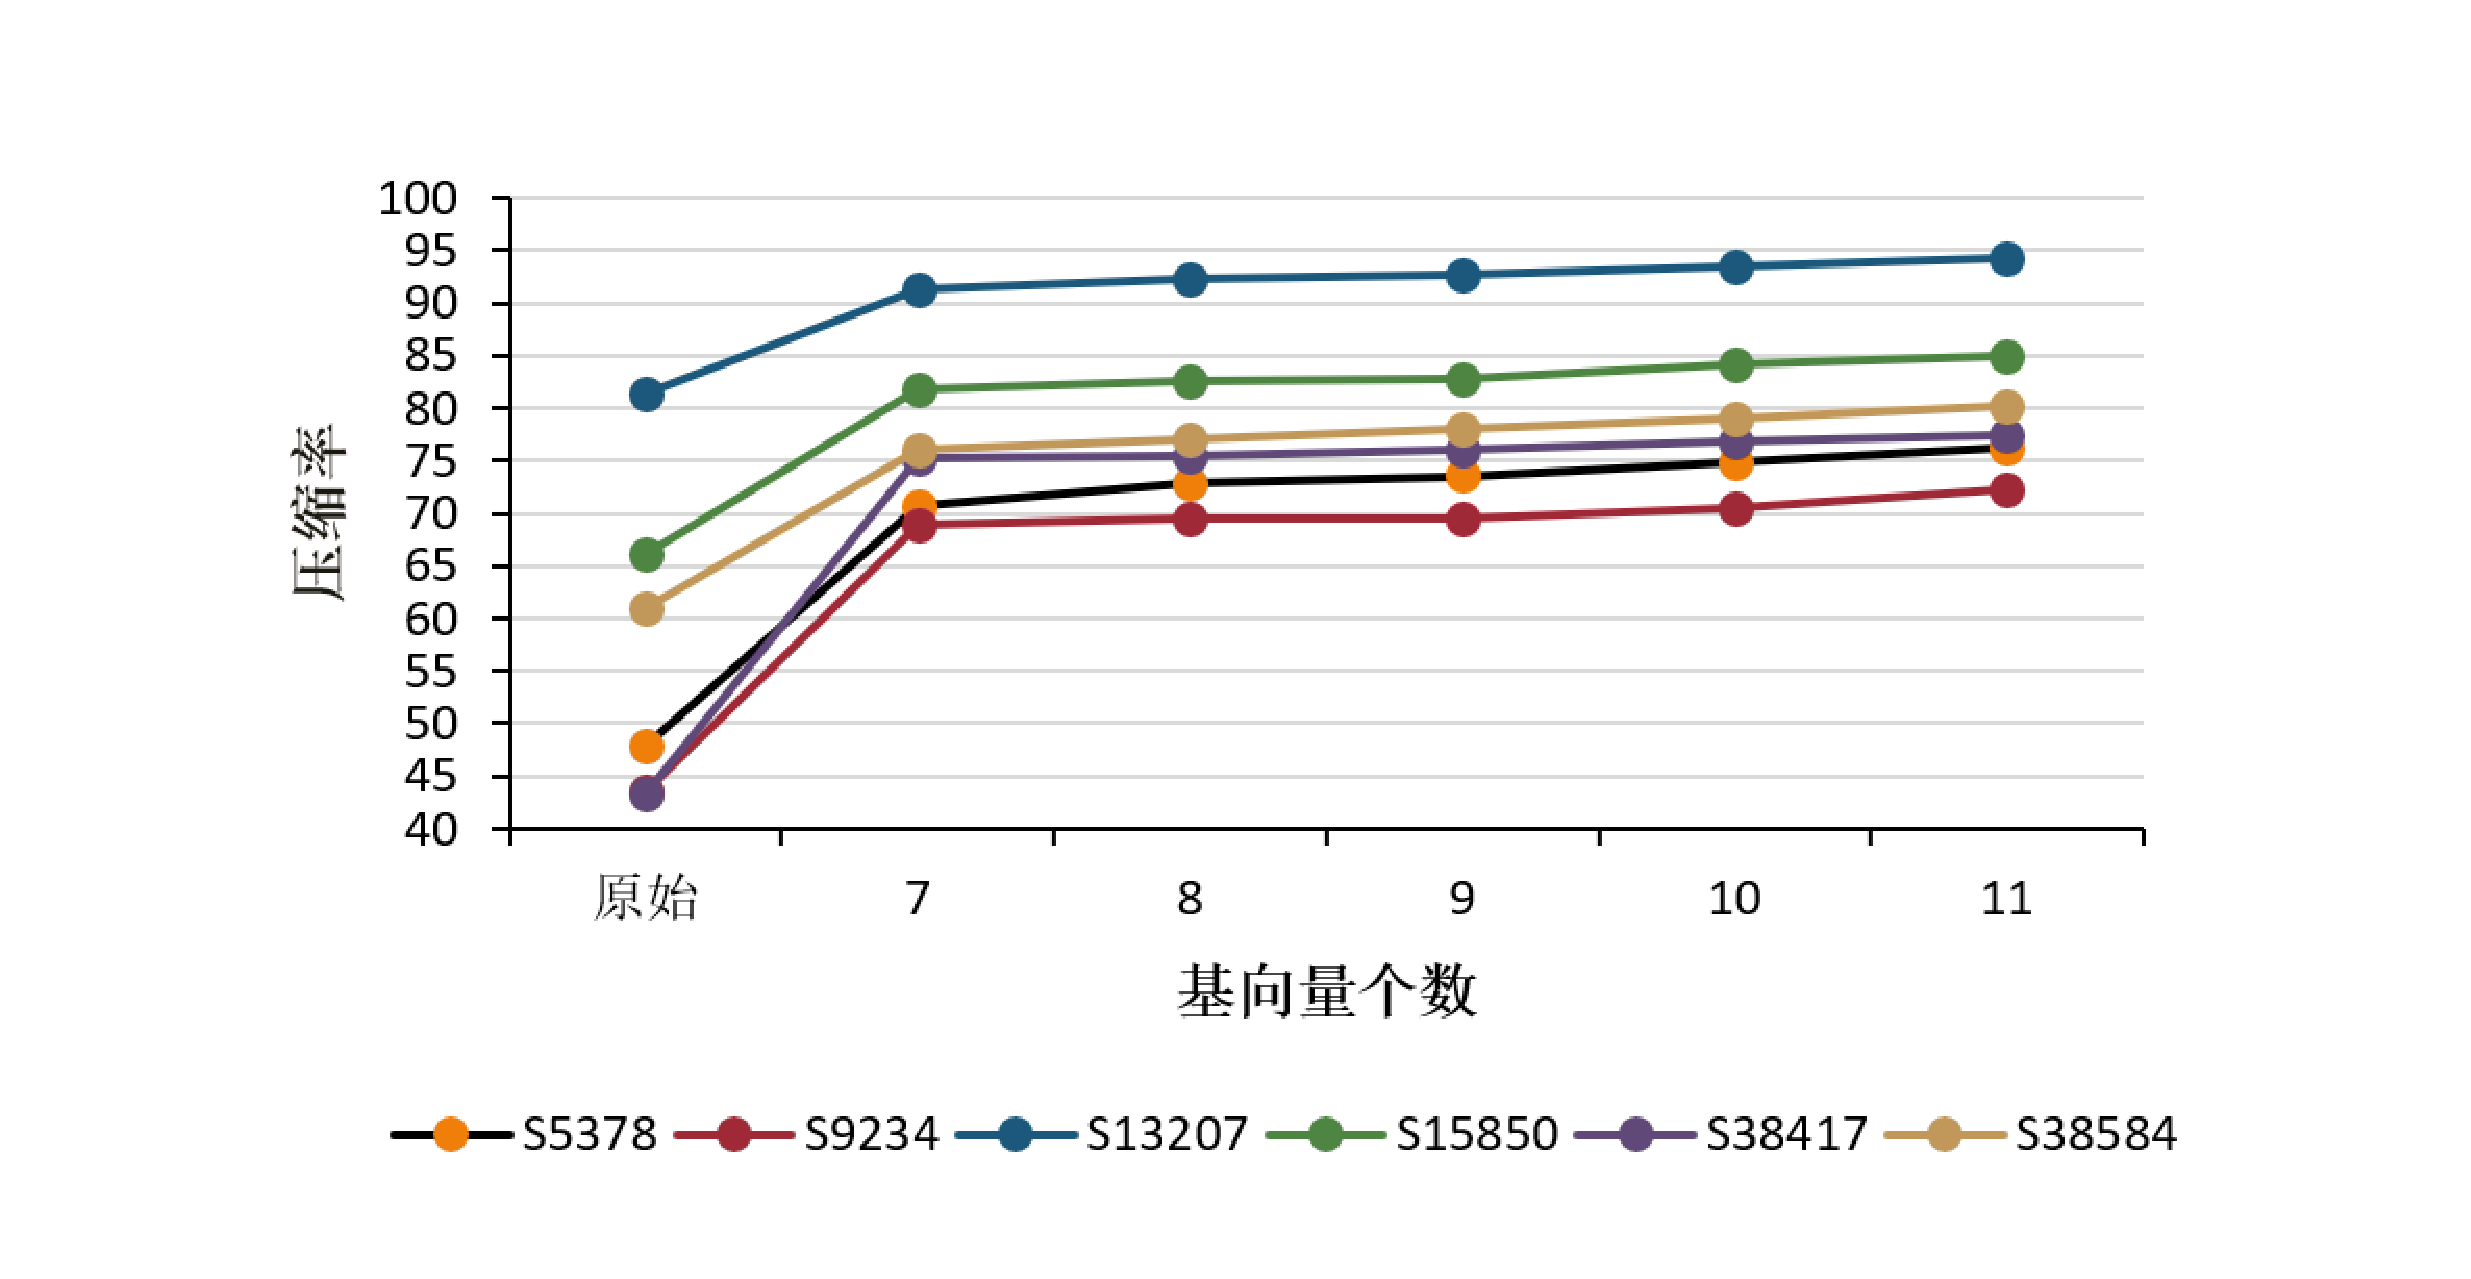
\includegraphics[height=8cm,width=16cm,angle=0,scale=1]{43.eps}
  \caption{FDR编码方式折线图}\label{43}
     \end{figure}

下表\ref{ptabl11}、图\ref{44}是当前算法在VIHC编码方式下,压缩率的变化情况。

\begin{table}[H]
\centering
\caption{VIHC编码压缩率(\%)}\label{ptabl11}
\begin{tabular}{p{1.4cm}p{2cm}<{\centering}p{1.8cm}<{\centering}p{1.8cm}<{\centering}p{1.8cm}<{\centering}
p{1.8cm}<{\centering}p{1.8cm}<{\centering}}
\toprule
\textbf{电路名}&	\textbf{直接编码}& \textbf{7列}& \textbf{8列}& \textbf{9列}& \textbf{10列}& \textbf{11列}\\
\midrule
s5378&	51.75&	72.81&	75.18&	76.02&	77.68&	78.97\\
s9234&	47.23&	72.35&	73.25&	73.4&	74.33&	75.98\\
s13207&	83.55&	93.42&	94.2&	94.55&	95.01&	95.71\\
s15850&	67.97&	84.82&	85.28&	85.42&	86.8&	87.47\\
s38417&	53.39&	77.86&	78.17&	78.64&	79.23&	79.73\\
s38584&	62.30& 	78.42&	79.25&	80.51&	81.62&	82.72\\
平均&	61.03&	79.95&	80.89&	81.42&	82.445&	83.43\\
\bottomrule
\end{tabular}
\end{table}

\begin{figure}[H]
  \centering
  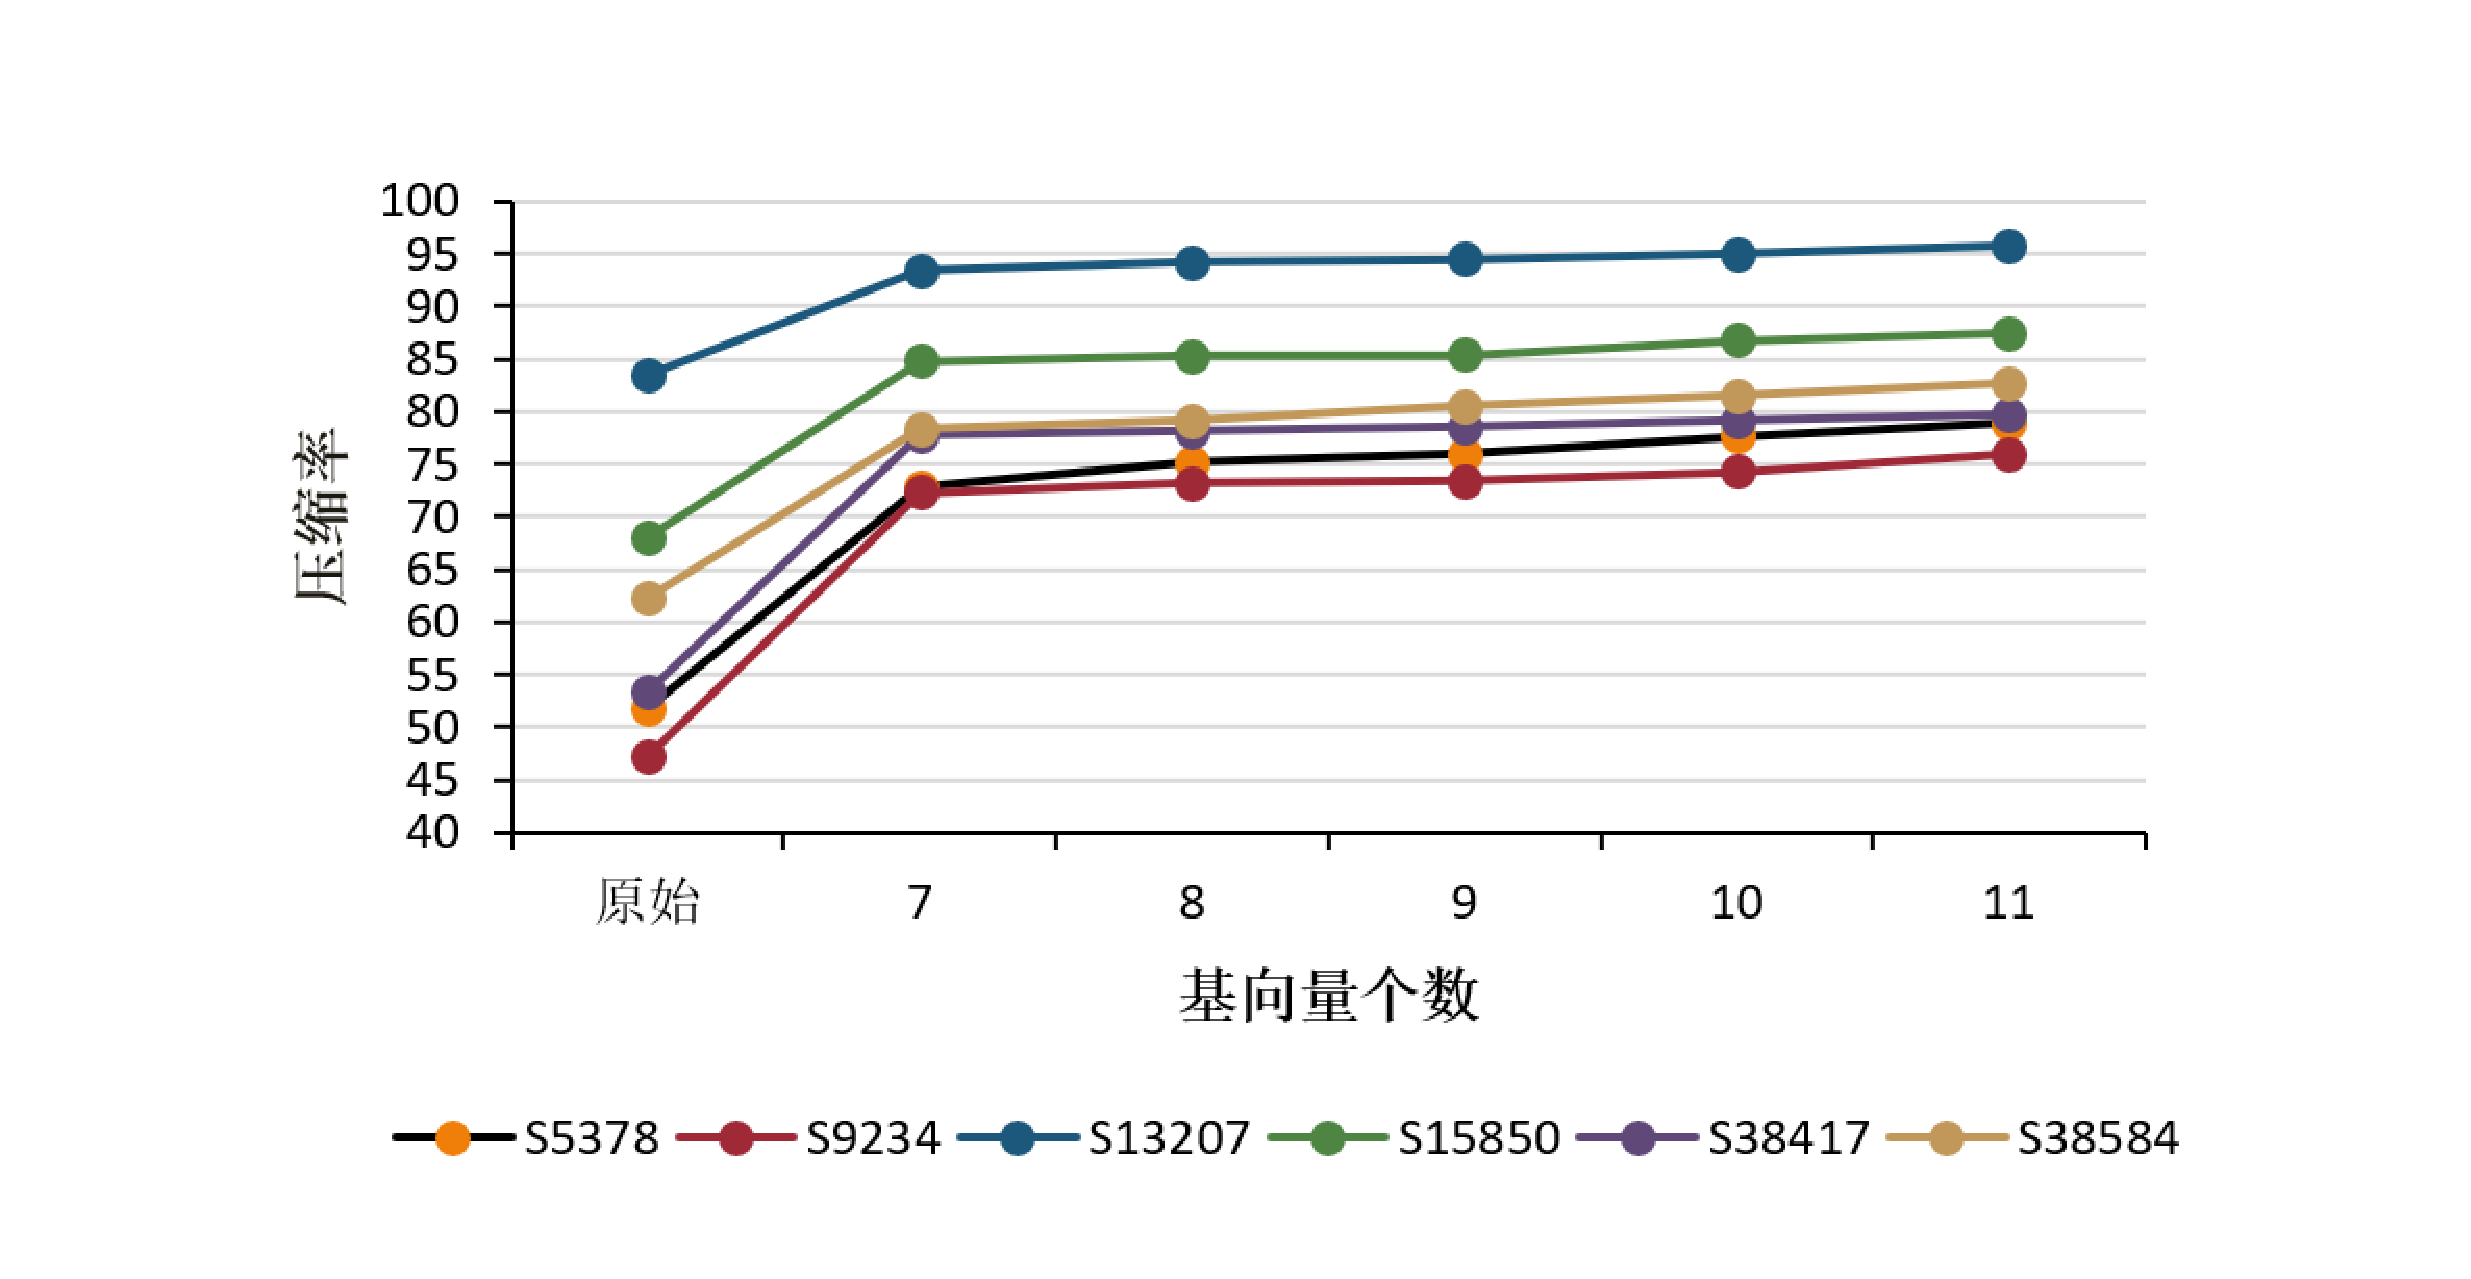
\includegraphics[height=8cm,width=16cm,angle=0,scale=1]{44.eps}
  \caption{VIHC编码方式折线图}\label{44}
     \end{figure}

下表\ref{ptabl12}-\ref{ptabl13}以及图\ref{45}、\ref{46}分别为当前算法在RL\_Huff、AFDR编码下压缩率的变化情况。

\begin{table}[H]
\centering
\caption{RL\_Huff编码压缩率(\%)}\label{ptabl12}
\begin{tabular}{p{1.4cm}p{2cm}<{\centering}p{1.8cm}<{\centering}p{1.8cm}<{\centering}p{1.8cm}<{\centering}
p{1.8cm}<{\centering}p{1.8cm}<{\centering}}
\toprule
\textbf{电路名}&	\textbf{直接编码}& \textbf{7列}& \textbf{8列}& \textbf{9列}& \textbf{10列}& \textbf{11列}\\
\midrule
s5378&	52.58&  68.59&	71.26&	71.79&	73.59&	74.91\\
s9234&	47.26&  66.05&	67.07&	67.05&	68.17&	70.18\\
s13207&	82.94&  91.81&	92.82&	93.23&	93.79&	94.62\\
s15850&	67.35&  80.57&	81.73&	81.77&	83.65&	84.34\\
s38417&	63.32&  74.02&	74.28&	74.71&	75.57&	76.17\\
s38584&	62.40&  73.70&	74.74&	76.13&	77.42&	78.78\\
平均&	62.64&  75.79&	76.98&	77.45&	78.70&	79.83\\
\bottomrule
\end{tabular}
\end{table}

\begin{figure}[H]
  \centering
  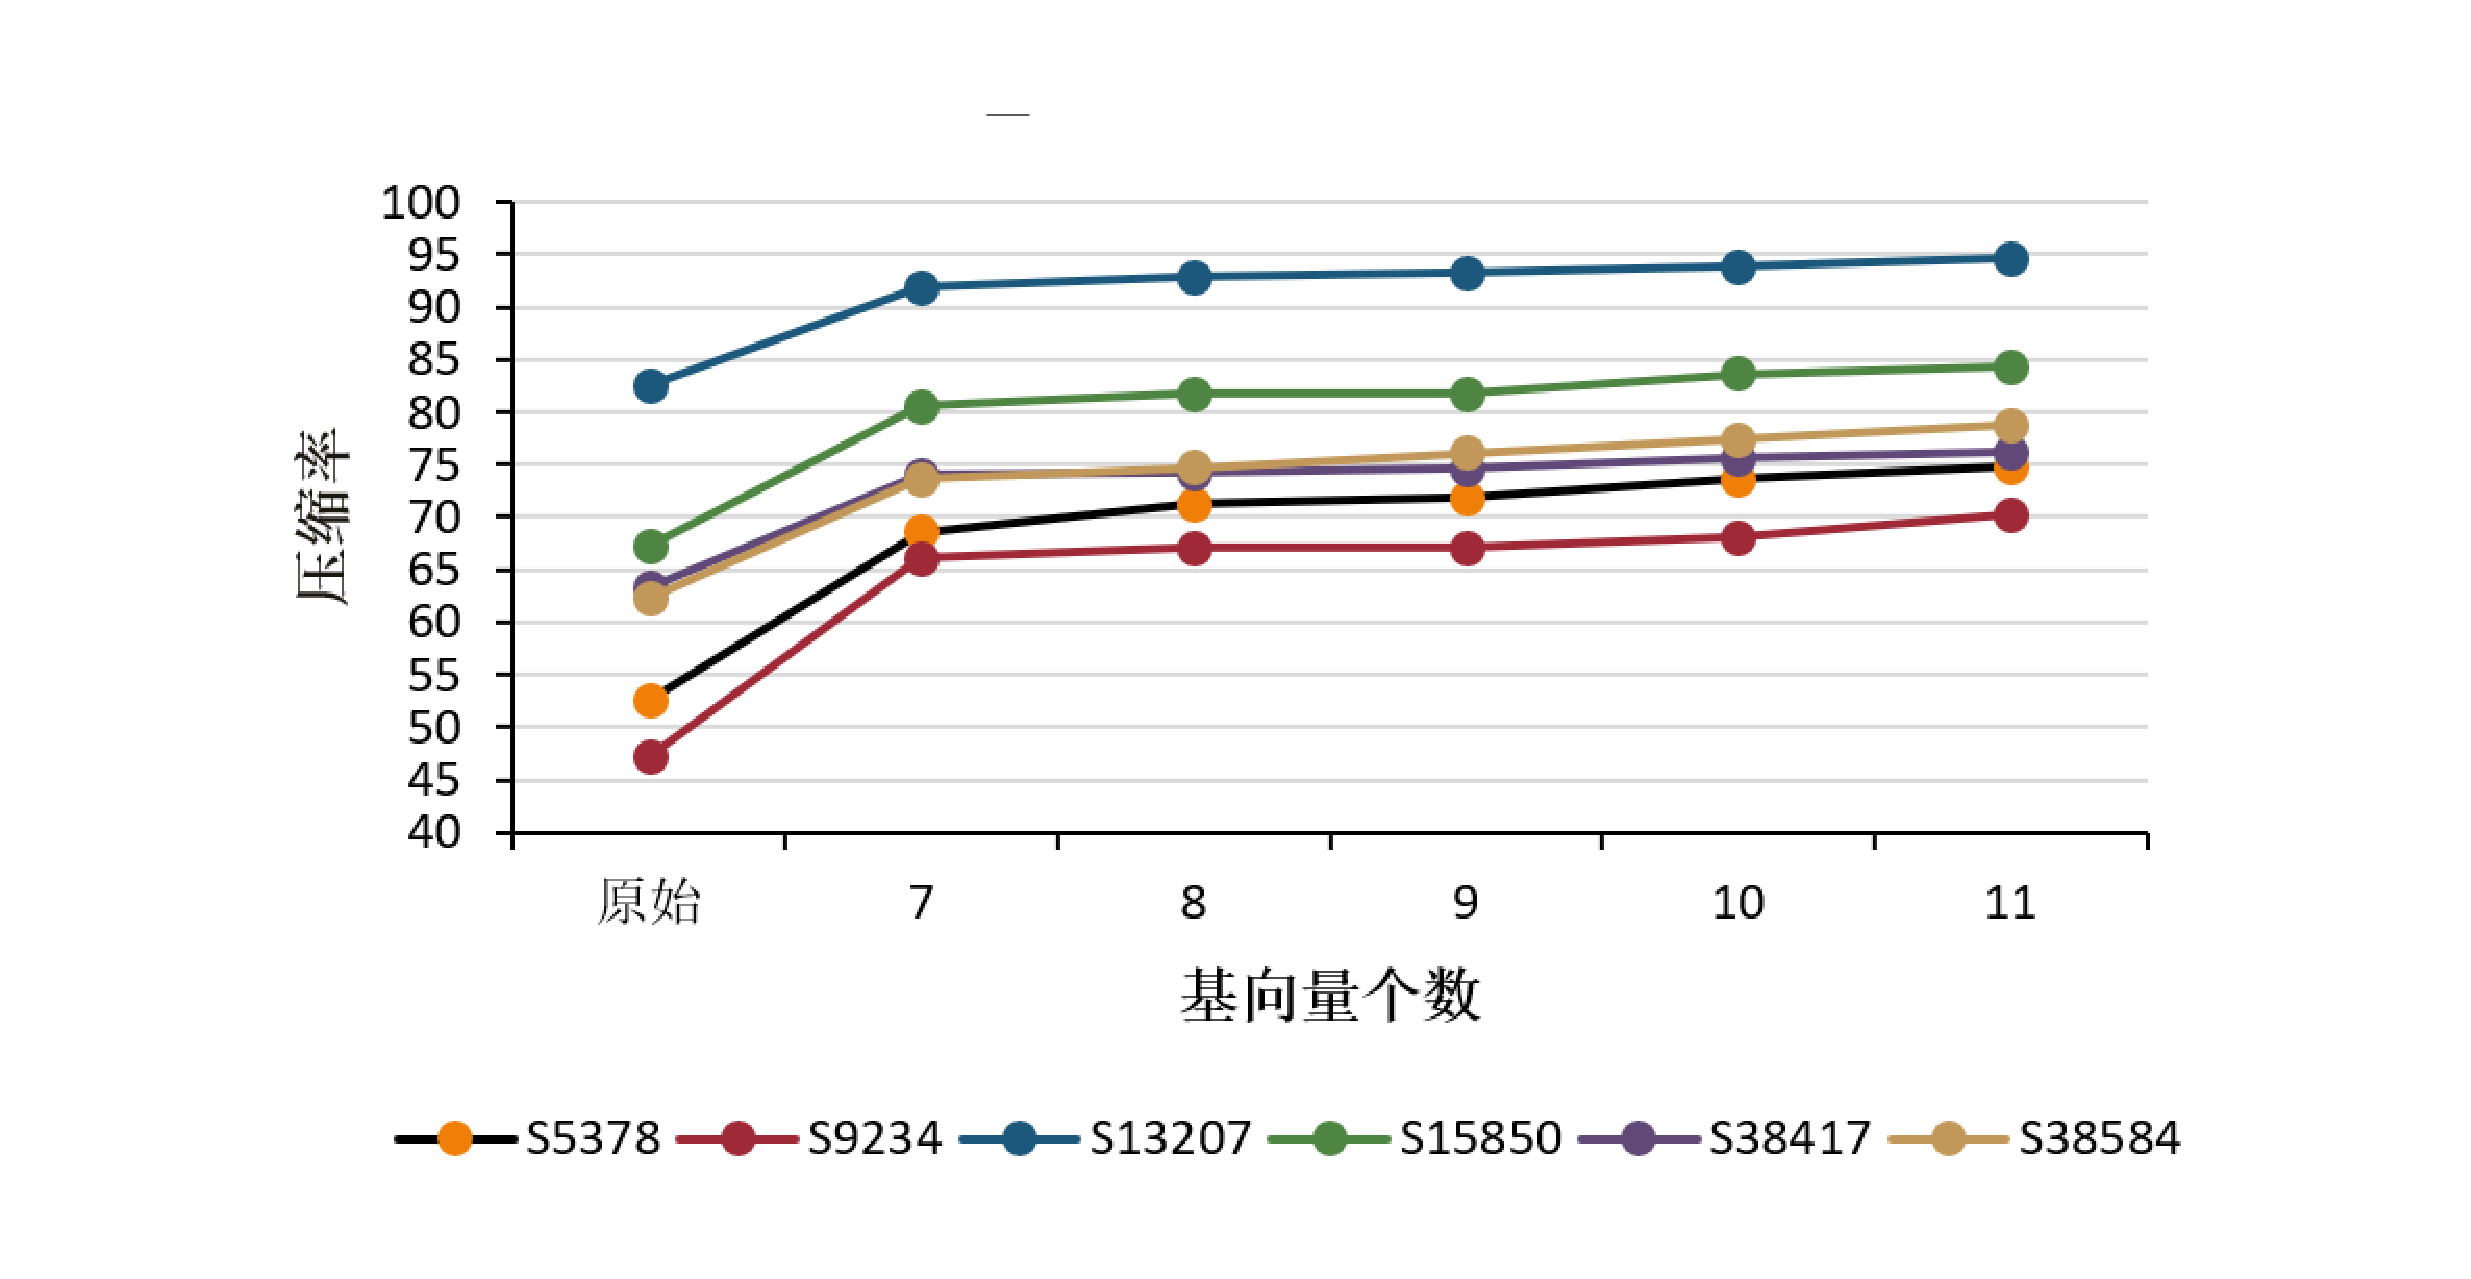
\includegraphics[height=8cm,width=16cm,angle=0,scale=1]{45.eps}
  \caption{RL\_Huff编码方式折线图}\label{45}
     \end{figure}


\begin{table}[H]
\centering
\caption{AFDR编码压缩率(\%)}\label{ptabl13}
\begin{tabular}{p{1.4cm}p{2cm}<{\centering}p{1.8cm}<{\centering}p{1.8cm}<{\centering}p{1.8cm}<{\centering}
p{1.8cm}<{\centering}p{1.8cm}<{\centering}}
\toprule
\textbf{电路名}&	\textbf{直接编码}& \textbf{7列}& \textbf{8列}& \textbf{9列}& \textbf{10列}& \textbf{11列}\\
\midrule
s5378&	49.95&	65.17&	67.66&	68.72&	69.85&	71.53\\
s9234&	45.14&	61.78&	62.72&	63.06&	63.91&	66.11\\
s13207&	80.12&	89.66&	90.88&	91.45&	92.24&	93.18\\
s15850&	65.64&	77.82&	78.96&	78.99&	81.01&	81.66\\
s38417&	60.52&	71.23&	71.38&	71.97&	72.77&	73.34\\
s38584&	61.09&	70.82&	71.97&	73.29&	74.57&	75.93\\
平均&	60.41&	72.75&	73.93&	74.58&	75.73&	76.96\\
\bottomrule
\end{tabular}
\end{table}

\begin{figure}[H]
  \centering
  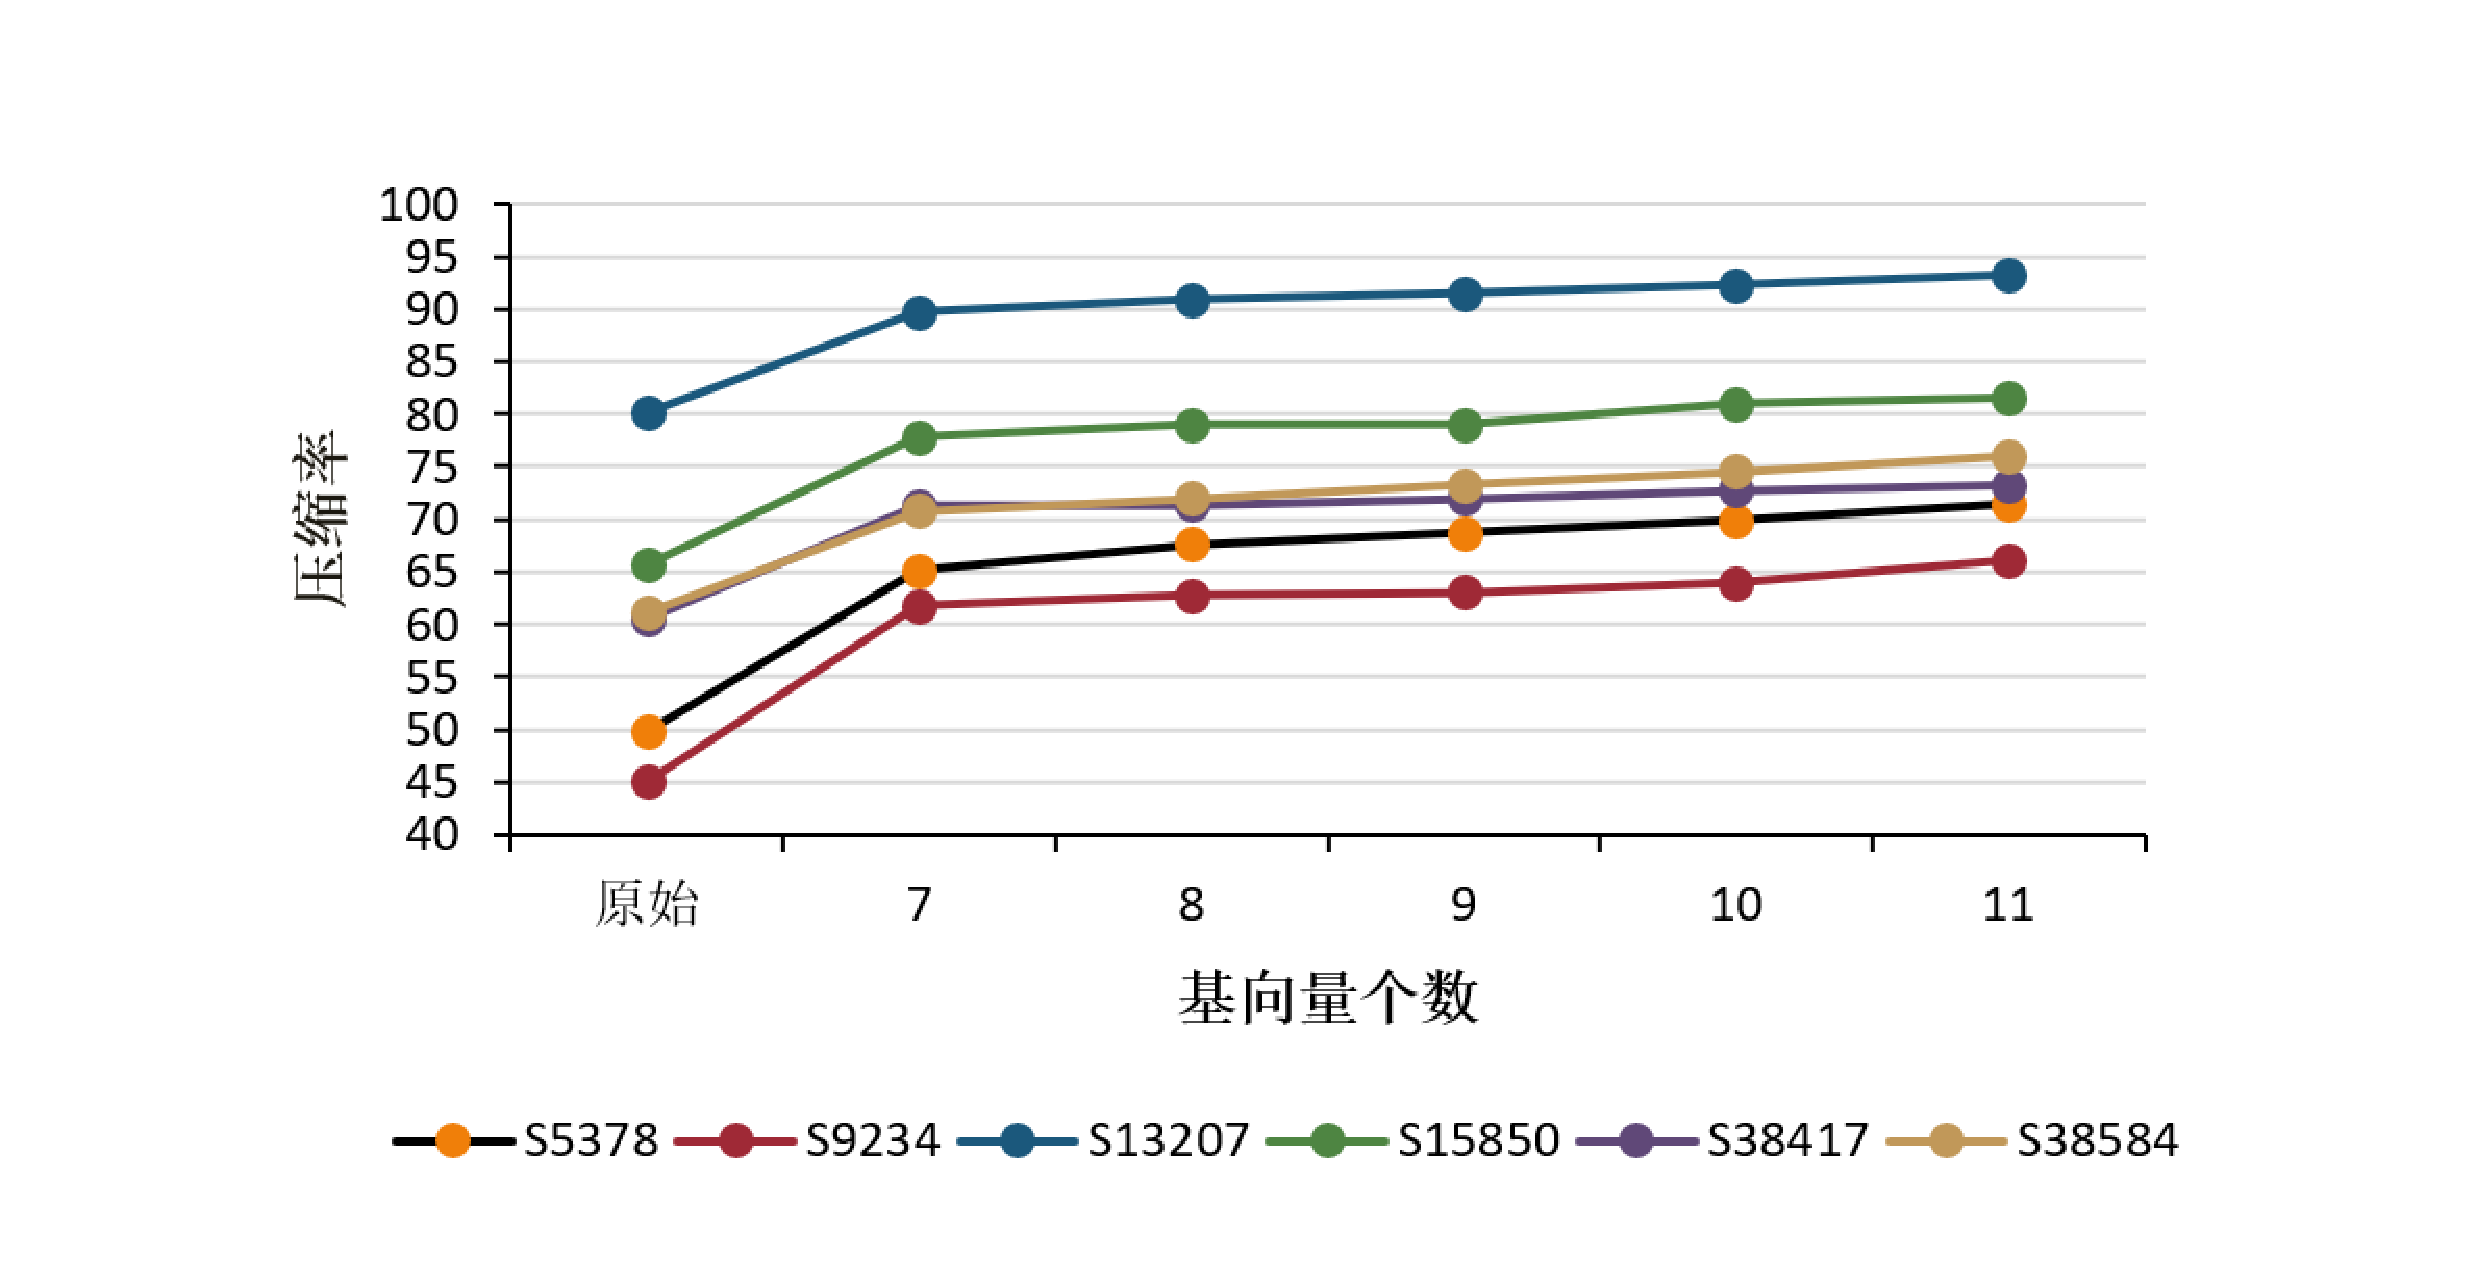
\includegraphics[height=8cm,width=16cm,angle=0,scale=1]{46.eps}
  \caption{AFDR编码方式折线图}\label{46}
     \end{figure}

从上述的折线图可知,随着选取基向量个数的增加,压缩率呈上升趋势,仔细观察可以发现,当基向量增加一个,压缩率提升百分之1左右。总而言之,当前压缩方法无论是根据电路大小确定基向量,还是动态选取基向量均能取得不错的压缩效果。

\section{小结}

本章提出了一种使用聚类算法结合原测试生成主分量的数据压缩方法,该方法先通过预填充方法,去除原测试集中的无关位,然后根据电路大小确定基向量数。由于初始基向量的个数会影响最终的压缩率,并且无法确定初始聚类数,本人进行了动态选取基向量数的相关实验,同时也使用当前压缩方法对大电路测试集进行了压缩。实验结果表明,使用kmeans++聚类算法集合原测试的压缩方法能大大提高压缩率。

% !Mode:: "TeX:UTF-8"

\chapter{使用kmeasn++算法结合位翻转算法进一步提高压缩率}

测试立方压缩旨在通过提高压缩率,降低测试时间、节约压缩成本。测试立方由一系列0、1以及无关位$X$组成,其中$X$ 既可以被填充为0 也可以被填充为1,而不影响原测试集的故障覆盖率,因此包含较多无关位的测试集往往会获得较高的压缩率。本章将使用位翻转算法在不影响故障覆盖率的前提下,通过增加原测试集的无关位提高压缩率。

\section{相关概念}

\subsection{故障检测冗余度}
故障检测冗余度通俗的来说就是同一个故障在测试过程中被多次检测。比如,数据冗余是指某个数据在特定情况下反复出现,那么故障检测冗余度类也是类似的。测试集由ATPG产生,初始测试集中包含大量数据,其中存在众多的无关位。由于可以将部分无关位会被转化成为确定位,测试集的规模会大大减小,但测试立方整体的故障覆盖率保持不变。

\subsection{位翻转}
本文主使用拆分压缩的方式提高压缩率,拆分压缩会将原测试立方拆分成为主分量集和残分量集,如果主分量集和原测试集高度相似便会提高残分量集的压缩率。假设主分量的故障覆盖率为$A$,测试立方的总故障覆盖率为$C$,剩余故障覆盖率为$C-A$。通过故障模拟之后原测试立方只要能检测出剩余故障即可,为了避免相同故障被反复检测可以将原测试立方中特定的确定位翻转为$X$,在总故障覆盖率不变的情况下,提高压缩率。这个过程被称之为位翻转。

\subsection{位翻转应用于压缩}
原测试集中包含的确定位会影响最终的压缩率,如果可以将部分确定位翻转成为无关位,将无关位按照有利于压缩的方向填充便能提高压缩率。为了降低硬件开销以及实验复杂度本人使用的是一轮位翻转,具体过程分为下述几个步骤:1、结合第三章与第四章的算法将原测试拆分成为主分量集和残差集。2、将主分量集进行故障模拟,记录能检测的故障数$A$,在不影响故障覆盖率的前提下将原测试集中的某些确定位翻转成为无关位$X$,生成新的测试集。3、将新的测试中的无关位进行填充然后与原主分量集进行异或,在本实验中无关位的填充方式主要根据主分量集对应的位进行填充。

下图\ref{51}为位翻转应结合本实验的压缩过程:图中可以看出原测试立方的故障覆盖率达100\%,拆分压缩之后的主分量集能取得的故障覆盖率可达到70\%,剩余故障为30\%。在保证故障覆盖率的条件下,将原测试集部分确定位翻转为无关位并获得新测试集,根据主分量的确定位对原测试集的无关位进行填充,最后将主分量集与已填充的测试集进行异或得到最终需要进行压缩的新残差集。

\begin{figure}[H]
  \centering
  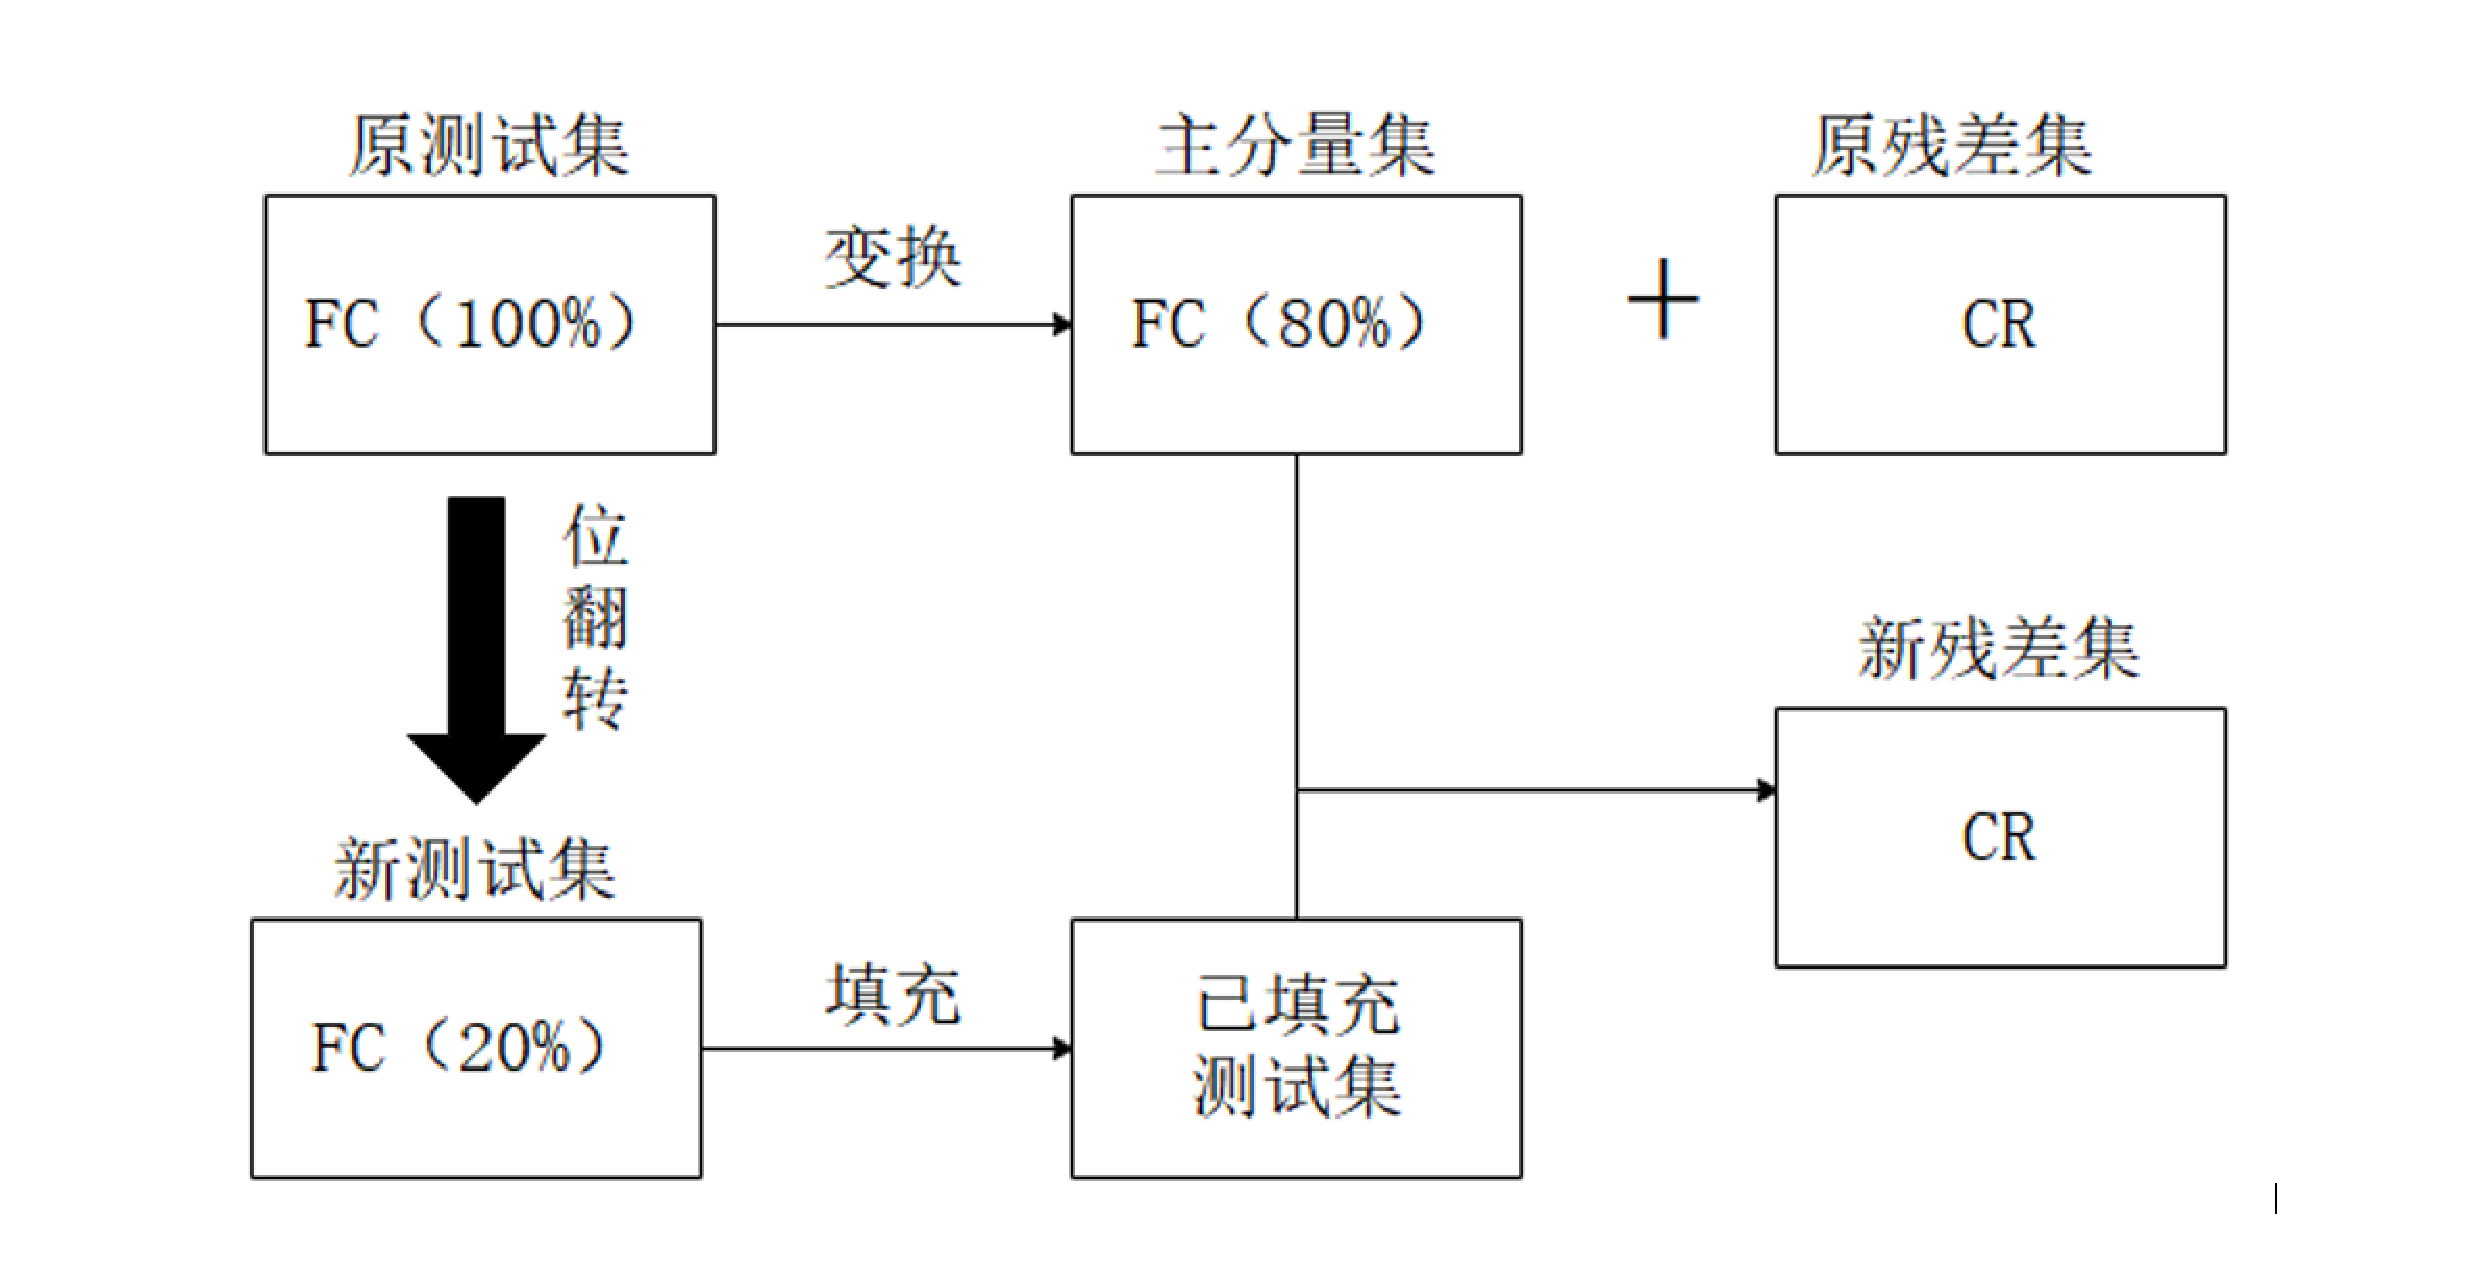
\includegraphics[height=8cm,width=16cm,angle=0,scale=1]{51.eps}
  \caption{FDR编码方式折线图}\label{51}
     \end{figure}

在论文“多次随机变换拆分测试激励压缩方法研究”\cite{76}中提及了多轮位翻转算法,但是由于每一轮翻转,均会产生代价,并且硬件代价与实现相对比较困难,本人化繁为简直接使用一轮压缩,然后根据主分量集对原测试集进行二次填充,在保证压缩率的前提下节约了硬件开销以及存储代价。

\section{翻转算法}
若$C$代表原测试集合的故障覆盖率,对原测试集进行位填充之后,拆分为主分量集和残差集,$A$代表主分量集合所能达到的故障覆盖率,假设原测试集合的故障覆盖率$B$,只需要满足$B>C-A$即可,下文将基于这种思路写出位翻转算法的伪代码。

\begin{algorithm}[!h]
	\caption{位翻转基本过程}%算法标题
	\begin{algorithmic}%一行一个标行号
        \STATE $CoverageC$  //原测试集的故障覆盖率
		\STATE $CoverageA$ $ $//拆分原测试集后主分量集的故障覆盖率
        \STATE $CoverageC$  $ \leftarrow $  $FaultCoverage$ $(T)$
        \STATE $CoverageB$  $ \leftarrow $  $FaultCoverage$ $(L)$
		\FOR{$bit$ in $T$}
        \IF{$bit$ = $1$ or $0$}
		\STATE $bit$  $ \leftarrow $  $X$
		\ENDIF
        \IF{$Coverage$ $<$ $CoverageA$ $-$ $CoverageB$}
		\STATE $bit$  $ \leftarrow $  $1$ $or$ $0$
		\ENDIF
		\ENDFOR
        \STATE $Return$ $T$
	\end{algorithmic}
\end{algorithm}

算法5.1为翻转测试集的基本过程,首先将原测试立方中的确定位一一翻转,并进行故障模拟,如果不影响故障覆盖率则直接翻转,反之还原,若故障模拟的时间为$t$,翻转一位的时间为$s$,假设原测试集合中由$k$个确定位,那么算法的时间复杂度为$kts$,理论上而言该算法可以通过较小的代价取得较高的压缩率。

\section{实验结果与分析}
为了说明kmeans++算法结合位翻转算法确实有效,本文对S5378、S9234、S13207、S15850等电路进行了实验。本章将挑选其中部分电路做具体描述,本文选取选取了FDR、EFDR、ALT-FDR编码方式对变换拆分之后的残差集进行压缩,同时与直接使用位翻转算法所达到的压缩率进行对比。

实验结果如下所示,表\ref{btabl1}-\ref{btabl3}分别表示各方法在FDR、EFDR、 ALT-FDR编码下缩能达到的压缩率,其中第一列为电路名称,第二列表示对测试集直接编码所能取得的压缩率,第三列表示使用原测试集集合kmeans++算法所能达到的压缩率,第四列表示对测试集直接翻转所达到的压缩率,第五列为使用本方法所达到的压缩率。

\begin{table}[H]
\centering
\caption{FDR编码压缩率(\%)}\label{btabl1}
\begin{tabular}{p{2.2cm}p{2.7cm}<{\centering}p{3.3cm}<{\centering}p{2.7cm}<{\centering}p{2.7cm}<{\centering}}
\toprule
\textbf{电路}&	\textbf{直接编码}& \textbf{Kmeans++聚类}& \textbf{直接翻转}& \textbf{本方法}\\
\midrule
s5378&	47.98&	70.76&	78.06&	79.69\\
s9234&	43.61&	69.59&	74.01&	78.06\\
s13207&	81.31&	92.29&	91.93&	94.93\\
s15850&	66.21&	81.75&	86.04&	86.27\\
s38417&	43.21&	75.35&	78.71&	80.31\\
平均&	56.46&	77.95&	81.75&	83.85\\
\bottomrule
\end{tabular}
\end{table}

\begin{table}[H]
\centering
\caption{EFDR编码压缩率(\%)}\label{btabl2}
\begin{tabular}{p{2.2cm}p{2.7cm}<{\centering}p{3.3cm}<{\centering}p{2.7cm}<{\centering}p{2.7cm}<{\centering}}
\toprule
\textbf{电路}&	\textbf{直接编码}& \textbf{Kmenas++聚类}& \textbf{直接翻转}& \textbf{本方法}\\
\midrule
s5378&	53.67&	67.75&	76.16&	77.68\\
s9234&	48.66&	66.14&	71.28&	75.85\\
s13207&	82.49&	91.60&	91.53&	94.52\\
s15850&	68.66&	79.84&	84.24&	84.99\\
s38417&	62.02&	74.06&	78.24&	79.13\\
平均&	63.0&	75.88&	80.29&	82.43\\
\bottomrule
\end{tabular}
\end{table}

\begin{table}[H]
\centering
\caption{ALT-FDR编码压缩率(\%)}\label{btabl3}
\begin{tabular}{p{2.2cm}p{2.7cm}<{\centering}p{3.3cm}<{\centering}p{2.7cm}<{\centering}p{2.7cm}<{\centering}}
\toprule
\textbf{电路}&	\textbf{直接编码}& \textbf{Kmenas++聚类}& \textbf{直接翻转}& \textbf{本方法}\\
\midrule
s5378&	49.95&	65.17&	72.17&	76.26\\
s9234&	45.14&	62.72&	67.61&	73.50\\
s13207&	80.12&	90.88&	88.93&	94.09\\
s15850&	65.64&	77.82&	81.64&	83.85\\
s38417&	60.52&	71.23&	75.32&	76.93\\
平均&	60.27&	73.56&	77.13&	80.93\\
\bottomrule
\end{tabular}
\end{table}

从上表可以看出本方法能极大地提升残差集的压缩率,比对电路直接编码所达到的平均压缩率高22.49\%,比对原测试集直接翻转所取得的平均压缩率高2.68\%。

\section{小结}
位翻转方法旨在通过将确定位翻转为无关位来提高压缩率。由于主分量集自身可以检测出部分故障,原测试集只需检测剩余故障即可。通过故障模拟,原测试将某些确定位翻转为无关位后,得到了一个新测试集,新测试集填充无关位之后与主分量异或得到了新的残差集,此时的残差集包含的0比特位大大增加,能进一步提高压缩率。使用kmeans++算法集合位翻转的压缩方法,能使压缩率在第四章的基础上提高7\%。



%% !Mode:: "TeX:UTF-8"

alg:schedule\chapter{图片的插入方法}

\section{研究生毕业论文的插图规范}

图应有自明性。插图应与文字紧密配合,文图相符,内容正确。选图要力求精练,插图、照片应完整清晰。图中文字和数字等字号用宋体五号字。

机械工程图:采用第一角投影法,严格按照~GB4457---GB131-83《机械制图》标准规定。

数据流程图、程序流程图、系统流程图等按~GB1526-89~标准规定。

电气图:图形符号、文字符号等应符合有关标准的规定。

流程图:必须采用结构化程序并正确运用流程框图。

对无规定符号的图形应采用该行业的常用画法。

坐标图的坐标线均用细实线,粗细不得超过图中曲线,有数字标注的坐标图,必须注明坐标单位。

照片图要求主题和主要显示部分的轮廓鲜明,便于制版。如用放大或缩小的复制品,必须清晰,反差适中。照片上应有表示目的物尺寸的标度。

引用文献图表必须标注出处。

\subsection{图题及图中说明}
每个图均应有图题(由图序和图名组成),图名在图序之后空两格排写。图序按章编排,如第~1~章第一个插图的图号为“图~1-1”等。
图题置于图下,要求中文用宋体五号字,位置居中。有图注或其它说明时应置于图题之上。引用图应注明出处,在图题右上角加引用文献号。
图中若有分图时,分图题置于分图之下或图题之下,分图号用~a)、b)等表示。

图中各部分说明应采用中文(引用的外文图除外)或数字项号,各项文字说明置于图题之上(有分图题者,置于分图题之上)。

\subsection{插图编排}
插图之前,文中必须有关于本插图的提示,如“见图~1-1”、“如图~1-1~所示”等。插图与其图题为一个整体,不得拆开排写于两页。
插图处的该页空白不够排写该图整体时,则可将其后文字部分提前排写,将图移到次页。

\section{\LaTeX~中推荐使用的图片格式}
在~\LaTeX~中应用最多的图片格式是~EPS(Encapsulated PostScript)格式,它是一种专用的打印机描述语言,常用于印刷或打印输出。
EPS~格式图片可通过多种方式生成,这里介绍一款功能强大的免费图片处理软件———\href{http://www.imagemagick.org/}{ImageMagick},
此软件可将其它格式图片转换为~EPS~格式图片,同时还可以锐化图片,使图片的局部清晰一些。

此软件对图片的格式转换操作都是在命令提示符(cmd.exe)中实现的,可以通过“开始$\to$运行$\to$输入~cmd$\to$回车”或
“开始$\to$程序$\to$附件$\to$命令提示符”找到它。在命令提示符下,首先采用“盘符命令”或“cd~命令”将当前目录改为待处理图片所在的目录,
在此目录下就可通过~convert~命令将图片转换为~EPS~格式,其命令的语法格式为

\indent\verb|convert [可选参数] 原文件名.原扩展名 新文件名.eps|.

若~convert~命令中无可选参数,则将原来的图片格式直接转换为~EPS~格式,对图片不进行任何处理,这也是最常用的方法。
也可以选用可选参数,可选参数有很多选择,但最常用的有如下两个:

\verb|-sharpen radius{xsigma}|———此参数用来锐化图片,一般用在图片像素不高,需要提高图片清晰度的情况下。其中~radius~只能为整数,
它用来确定转换命令采取哪一种锐化算法,我们可以只取~radius~为~0;sigma~为所采取算法的锐化度,它的取值为~$0.1 - 3$~之间的任意一个浮点数,
数值越大,锐化程度也越大,通常取为~$0.1 - 3$~之间;x~在参数中为分隔符。

\verb|-resize geometry|———此参数用来改变图片的大小,若图片的存储空间过大,可通过此命令缩小图片尺寸,但同时也将导致图片像素降低,
其具体用法请参见\href{http://www.imagemagick.org/script/command-line-options.php#resize}{-resize geometry~的官方说明}。

除此之外,一些文字处理软件和科学计算软件也支持生成~EPS~格式的文件,请使用“另存为”功能查看某款软件是否能够将图片以~EPS~ 格式的形式保存。

\section{单张图片的插入方法}
单张图片独自占一行的插入形式如图~\ref{fig:xml}~所示。
\begin{figure}[htbp]
\centering
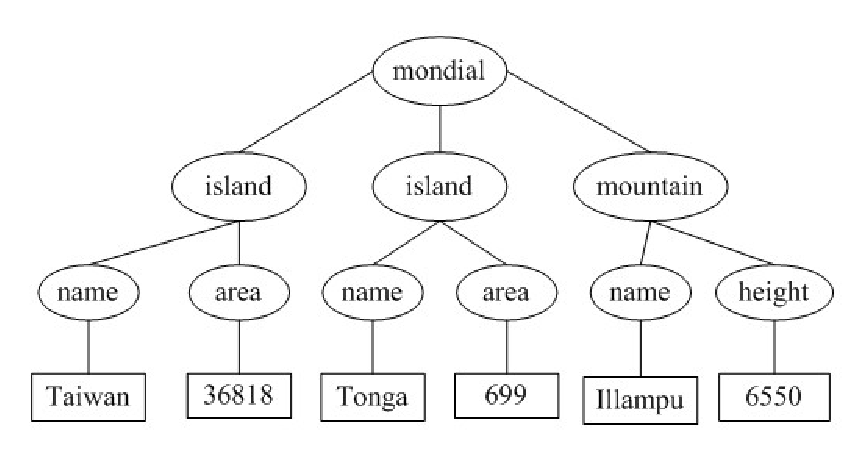
\includegraphics[width=0.4\textwidth]{XML}
\caption{树状结构}\label{fig:xml}
\vspace{\baselineskip}
\end{figure}


其插入图片的代码及其说明如下。
\vspace{1em}\noindent\hrule
\begin{verbatim}
\begin{figure}[htbp]
\centering
\includegraphics[width=0.4\textwidth]{文件名(.eps)}
\caption{标题}\label{标签名(通常为 fig:labelname)}
\vspace{\baselineskip} %表示图与正文空一行
\end{figure}
\end{verbatim}

\noindent\hrule

\begin{verbatim}
figure环境的可选参数[htbp]表示浮动图形所放置的位置,h (here)表示当前位置,t (top)表示页芯顶部,b (bottom)表示页芯底部,p (page)表示单独一页。在Word等软件中,图片通常插入到当前位置,如果当前页的剩余空间不够,图片将被移动到下一页,当前页就会出现很大的空白,其人工调整工作非常不便。由LaTeX提供的浮动图片功能,总是会按h->t->b->p的次序处理选项中的字母,自动调整图片的位置,大大减轻了工作量。
\centering命令将后续内容转换成每行皆居中的格式。
"\includegraphics"的可选参数用来设置图片插入文中的水平宽度,一般表示为正文宽度(\textwidth)的倍数。
\caption命令可选参数“标签名”为英文形式,一般不以图片或表格的数字顺序作为标签,而应包含一定的图片或表格信息,以便于文中引用(若图片、表格、公式、章节和参考文献等在文中出现的先后顺序发生了变化,其标注序号及其文中引用序号也会跟着发生变化,这一点是Word等软件所不能做到的)。另外,图题或表题并不会因为分页而与图片或表格体分置于两页,章节等各级标题也不会置于某页的最底部,LaTeX系统会自动调整它们在正文中的位置,这也是Word等软件所无法匹敌的。
\vspace将产生一定高度的竖直空白,必选参数为负值表示将后续文字位置向上提升,参数值可自行调整。em为长度单位,相当于大写字母M的宽度。\vspace{\baselineskip} 表示图与正文空一行。
引用方法:“见图~\ref{fig:figname}”、“如图~\ref{fig:figname}~所示”等。
\end{verbatim}

\noindent\hrule\vspace{1em}

若需要将~2~张及以上的图片并排插入到一行中,则需要采用\verb|minipage|环境,如图~\ref{fig:dd}~和图~\ref{fig:ds}~所示。
\begin{figure}[htbp]
\centering
\begin{minipage}{0.4\textwidth}
\centering
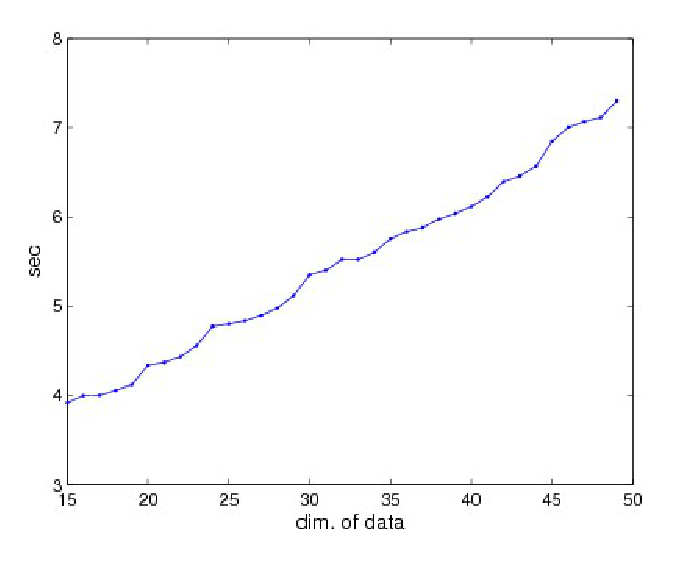
\includegraphics[width=\textwidth]{dataDimensions}
\caption{数据维数的变化}\label{fig:dd}
\end{minipage}
\begin{minipage}{0.4\textwidth}
\centering
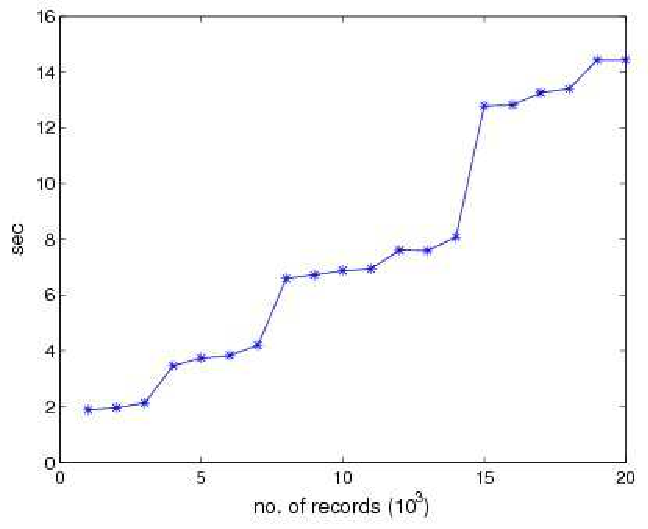
\includegraphics[width=\textwidth]{dataSize}
\caption{数据规模的变化}\label{fig:ds}
\end{minipage}
\vspace{\baselineskip}
\end{figure}

其代码如下所示。
\vspace{1em}\noindent\hrule
\begin{verbatim}
\begin{figure}[htbp]
\centering
\begin{minipage}{0.4\textwidth}
\centering
\includegraphics[width=\textwidth]{文件名}
\caption{标题}\label{fig:f1}
\end{minipage}
\begin{minipage}{0.4\textwidth}
\centering
\includegraphics[width=\textwidth]{文件名}
\caption{标题}\label{fig:f2}
\end{minipage}\vspace{\baselineskip}
\end{figure}
\end{verbatim}

\noindent\hrule

\begin{verbatim}
minipage环境的必选参数用来设置小页的宽度,若需要在一行中插入n个等宽图片,则每个小页的宽度应略小于(1/n)\textwidth。
\end{verbatim}

\noindent\hrule

\section{具有子图的图片插入方法}

图中若含有子图时,需要调用~subfigure~宏包, 如图~\ref{fig:subfig}~所示。
\begin{figure}[htbp]
  \centering
  \subfigure[Data Dimensions]{\label{fig:subfig:datadim}
                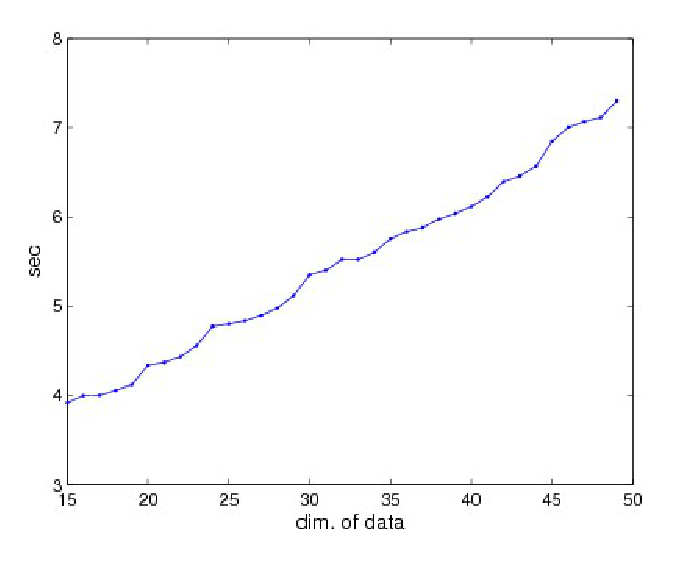
\includegraphics[width=0.4\textwidth]{dataDimensions}}
  \subfigure[Data Size]{\label{fig:subfig:datasize}
                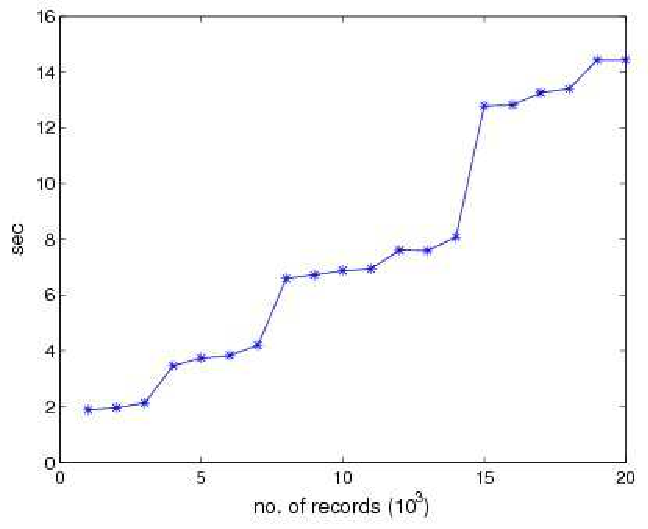
\includegraphics[width=0.4\textwidth]{dataSize}}
  \caption{Scalability of data}\label{fig:subfig}
\vspace{\baselineskip}
\end{figure}

其代码及其说明如下。
\vspace{1em}\noindent\hrule

\begin{verbatim}
\begin{figure}[htbp]
  \centering
  \subfigure[第1个子图标题]{
            \label{第1个子图标签(通常为 fig:subfig1:subsubfig1)}
            \includegraphics[width=0.4\textwidth]{文件名}}
  \subfigure[第2个子图标题]{
            \label{第2个子图标签(通常为 fig:subfig1:subsubfig2)}
            \includegraphics[width=0.4\textwidth]{文件名}}
  \caption{总标题}\label{总标签(通常为 fig:subfig1)}
\vspace{\baselineskip}
\end{figure}
\end{verbatim}

\noindent\hrule

\begin{verbatim}
子图的标签实际上可以随意设定,只要不重复就行。但为了更好的可读性,我们建议fig:subfig:subsubfig格式命名,这样我们从标签名就可以知道这是一个子图引用。
引用方法:总图的引用方法同本章第1节,子图的引用方法用\ref{fig:subfig:subsubfig}来代替。
\end{verbatim}

\noindent\hrule\vspace{1em}

子图的引用示例:如图~\ref{fig:subfig:datadim}~和图~\ref{fig:subfig:datasize}~所示。

若想获得插图方法的更多信息,参见网络上的~\href{ftp://ftp.tex.ac.uk/tex-archive/info/epslatex.pdf}{Using Imported Graphics in \LaTeX and pdf\LaTeX}~文档。

\section{插入算法}

\begin{algorithm}[!h]
{
{
\renewcommand\baselinestretch{1.5}\selectfont %控制行距
\caption{ Scheduling Algorithm }
\label{alg:schedule}
\begin{algorithmic}[1]
\REQUIRE ~\\
A DFG $G=<V,E>$;\\
An allocation $A(G)$ for $G$.
\ENSURE ~\\
A schedule.
    \STATE{.......................}
    \FOR{$i\leftarrow\ 1\ to\ M$}
        \STATE{.......................}
    \ENDFOR
    \STATE{.......................}
    \STATE{.......................}
    \STATE{.......................}
    \STATE{.......................}
    \STATE{.......................}
    \FOR{$k\leftarrow\ 1\ to\ |V|$}
        \STATE{.......................}
        \STATE{.......................}
        \STATE{.......................}
        \STATE{.......................}
    \IF{$LT_k==j$}
        \IF{there is no idle core in cluster $cl_{loc}$}
            \STATE{.......................}
            \STATE{.......................}
            \STATE{.......................}
            \STATE{.......................}
            \STATE{.......................}
            \STATE{.......................}
        \ELSE
            \STATE{.......................}
            \STATE{.......................}
            \STATE{.......................}
            \STATE{.......................}
            \STATE{.......................}
            \STATE{.......................}
        \ENDIF
    \ENDIF
    \ENDFOR


\end{algorithmic}
}
\par}
\end{algorithm}

%% !Mode:: "TeX:UTF-8"

\chapter{表格的绘制方法}
\section{研究生毕业设计论文的绘表规范}

表应有自明性。表格不加左、右边线。表的编排建议采用国际通行的三线表。表内中文书写使用宋体五号字。

每个表格之上均应有表题(由表序和表名组成)。表序一般按章编排,如第~1~章第一个插表的序号为“表~1-1”等。表序与表名之间空两格,
表名使用中文五号字,居中。表名中不允许使用标点符号,表名后不加标点。
表头设计应简单明了,尽量不用斜线。表头中可采用化学,物理量等专业符号。

全表如用同一单位,则将单位符号移至表头右上角,加圆括号\cite{djy}。
表中数据应准确无误,书写清楚。数字空缺的格内加横线“-”(占~2~个数字宽度)。表内文字或数字上、下或左、右相同时,
采用通栏处理方式,不允许用“〃”、“同上”之类的写法。

表内文字使用宋体五号字,垂直居中书写,起行空一格、转行顶格、句末不加标点。
如某个表需要转页接排,在随后的各页上应重复表的编号。编号后加“(续表)”,表题可省略。续表应重复表头。
表格绘制完成之后,与正文空一行。

\section{普通表格的绘制方法}

表格应具有三线表格式,因此需要调用~booktabs~宏包,其标准格式如表~\ref{tab:table1}~所示。

\renewcommand\arraystretch{1.5}%控制行距
\begin{table}[!h]
\caption{基准测试集参数}\label{tab:bench}
\vspace{0.5em}
\centering
\begin{tabular}{l*{1}{C{2cm}}*{1}{L{6.2cm}}}
\toprule
Name         & $n$ & Description\\
\midrule
Random1      & 50  & Random graph generated by TGFF\\
Random2      & 100 & Random graph generated by TGFF\\
Random3      & 150 & Random graph generated by TGFF\\
Random4      & 200 & Random graph generated by TGFF\\
Random5      & 250 & Random graph generated by TGFF\\
Random6      & 300 & Random graph generated by TGFF\\
Random7      & 350 & Random graph generated by TGFF\\
Random8      & 400 & Random graph generated by TGFF\\
Random9      & 450 & Random graph generated by TGFF\\
Random10     & 500 & Random graph generated by TGFF\\
\bottomrule
\end{tabular}
\vspace{\baselineskip}
\end{table}
\renewcommand\arraystretch{1}

其绘制表格的代码及其说明如下。
\vspace{1em}\noindent\hrule

\begin{verbatim}
\begin{table}[htbp]
\caption{表标题}\label{标签名(通常为 tab:tablename)}
\vspace{0.5em}\centering\wuhao
\begin{tabular}{cc...c}
\toprule[1.5pt]
表头第1个格   & 表头第2个格   & ... & 表头第n个格  \\
\midrule[1pt]
表中数据(1,1) & 表中数据(1,2) & ... & 表中数据(1,n)\\
表中数据(2,1) & 表中数据(2,2) & ... & 表中数据(2,n)\\
表中数据(3,1) & 表中数据(3,2) & ... & 表中数据(3,n)\\
表中数据(4,1) & 表中数据(4,2) & ... & 表中数据(4,n)\\
...................................................\\
表中数据(m,1) & 表中数据(m,2) & ... & 表中数据(m,n)\\
\bottomrule[1.5pt]
\end{tabular}
\vspace{\baselineskip}
\end{table}
\end{verbatim}

\noindent\hrule

\begin{verbatim}
table环境是一个将表格嵌入文本的浮动环境。
\wuhao命令将表格的字号设置为五号字(10.5pt),在绘制表格结束退出时,不需要将字号再改回为\xiaosi,正文字号默认为小四号字(12pt)。
tabular环境的必选参数由每列对应一个格式字符所组成:c表示居中,l表示左对齐,r表示右对齐,其总个数应与表的列数相同。此外,@{文本}可以出现在任意两个上述的列格式之间,其中的文本将被插入每一行的同一位置。表格的各行以\\分隔,同一行的各列则以&分隔。
\toprule、\midrule和\bottomrule三个命令是由booktabs宏包提供的,其中\toprule和\bottomrule分别用来绘制表格的第一条(表格最顶部)和第三条(表格最底部)水平线,\midrule用来绘制第二条(表头之下)水平线,且第一条和第三条水平线的线宽为1.5pt,第二条水平线的线宽为1pt。
引用方法:“如表~\ref{tab:tablename}~所示”。
\end{verbatim}

\noindent\hrule

\section{长表格的绘制方法}

长表格是当表格在当前页排不下而需要转页接排的情况下所采用的一种表格环境。若长表格仍按照普通表格的绘制方法来获得,
其所使用的\verb|table|浮动环境无法实现表格的换页接排功能,表格下方过长部分会排在表格第1页的页脚以下。为了能够实现长表格的转页接排功能,
需要调用~longtable~宏包,由于长表格是跨页的文本内容,因此只需要单独的\verb|longtable|环境,所绘制的长表格的格式如表~\ref{tab:table2}~所示。

此长表格~\ref{tab:table2}~第~2~页的标题“编号(续表)”和表头是通过代码自动添加上去的,无需人工添加,若表格在页面中的竖直位置发生了变化,长表格在第~2~页
及之后各页的标题和表头位置能够始终处于各页的最顶部,也无需人工调整,\LaTeX~系统的这一优点是~Word~等软件所无法企及的。

下段内容是为了让下面的长表格分居两页,看到表标题“编号(续表)”的效果。摘录于《你若安好,便是晴天 -- 林徽因传》片段:

她叫林徽因,出生于杭州,是许多人梦中期待的白莲。她在雨雾之都伦敦,发生过一场空前绝后的康桥之恋。她爱过三个男子,爱得清醒,也爱得平静。徐志摩为她徜徉在康桥,深情地等待一场旧梦可以归来。梁思成与她携手走过千山万水,为完成使命而相约白头。金岳霖为她终身不娶,痴心不改地守候一世。可她懂得人生飘忽不定,要学会随遇而安。
真正的平静,不是避开车马喧嚣,而是在心中修篱种菊。尽管如流往事,每一天都涛声依旧,只要我们消除执念,便可寂静安然。愿每个人在纷呈世相中不会迷失荒径,可以端坐磐石上,醉倒落花前。
如果可以,请让我预支一段如莲的时光,哪怕将来某一天加倍偿还。这个雨季会在何时停歇,无从知晓。但我知道,你若安好,便是晴天。					 
\wuhao\begin{longtable}{ccc}
\caption{湖南大学各学院名称一览}\label{tab:table2}
 \vspace{0.5em}\\
\toprule[1.5pt] 学院名称 & 网址 & 联系电话  \\ \midrule[1pt]
\endfirsthead
\multicolumn{3}{c}{表~\thetable(续表)}\vspace{0.5em}\\
\toprule[1.5pt] 学院名称 & 网址 & 联系电话  \\ \midrule[1pt]
\endhead
\bottomrule[1.5pt]
\endfoot
机械工程学院& \url{http://tdjxxy.tju.edu.cn/}& 87401979\\
精密仪器与光电子工程学院&  \url{http://www2.tju.edu.cn/colleges/precision/cn/}& 27404775\\
电子信息工程学院& \url{http://www.tju.edu.cn/seie}& 27406956\\
电气与自动化工程学院& \url{http://www2.tju.edu.cn/colleges/automate/}& 27405477\\
建筑工程学院& \url{http://www2.tju.edu.cn/colleges/civil/}& 27404072\\
化工学院& \url{http://chemeng.tju.edu.cn/}& 27403389\\
材料科学与工程学院& \url{http://mse.tju.edu.cn}& 27406693 \\
建筑学院& \url{http://hgw022072.chinaw3.com/}& 27402724-2111\\
求是学部\\
管理与经济学部&	\url{ http://sm.tju.edu.cn}& 27403423\\
理学院& \url{ http://www.tju.edu.cn/science/}& 27404118\\
文法学院& \url{ http://www2.tju.edu.cn/colleges/sociology/new/}& 27403691\\
软件学院& \url{http://scs.tju.edu.cn}& 87401540\\
计算机科学与技术学院& \url{http://cs.tju.edu.cn/}& 27406538\\
马克思主义学院& \url{http://www2.tju.edu.cn/colleges/marxism/}& 27405348\\
环境科学与工程学院& \url{http://www.tju.edu.cn/see}& 87402072\\
药物科学与技术学院& \url{http://www2.tju.edu.cn/colleges/pharmtier/}& 87401830\\
教育学院& \url{http://soe.tju.edu.cn/}& 27401028\\
职业技术教育学院& \url{http://202.113.0.248:8888}\\
继续教育学院& \url{http://aectu.tju.edu.cn/}& 27406298\\
仁爱学院& \url{http://www.tjrac.edu.cn/}& 68579990\\
农业与生物工程学院& \url{http://202.113.13.169/site/nongxueyuan/}& 87402171\\
国际教育学院 & \url{http://www.ietju.com/}& 27406147\\
网络教育学院 & \url{http://www.etju.com/}& 27426952 \\

\end{longtable}\xiaosi
\vspace{\baselineskip}

绘制长表格的代码及其说明如下。
\vspace{1em}\noindent\hrule

\begin{verbatim}
\wuhao\begin{longtable}{cc...c}
\caption{表标题}\label{标签名(通常为 tab:tablename)}\\
\toprule[1.5pt] 表头第1个格 & 表头第2个格 & ... & 表头第n个格\\ \midrule[1pt]
\endfirsthead
\multicolumn{n}{c}{表~\thetable(续表)}\vspace{0.5em}\\
\toprule[1.5pt] 表头第1个格 & 表头第2个格 & ... & 表头第n个格\\ \midrule[1pt]
\endhead
\bottomrule[1.5pt]
\endfoot
表中数据(1,1) & 表中数据(1,2) & ... & 表中数据(1,n)\\
表中数据(2,1) & 表中数据(2,2) & ... & 表中数据(2,n)\\
...................................................\\
表中数据(m,1) & 表中数据(m,2) & ... & 表中数据(m,n)\\
\end{longtable}\xiaosi
\end{verbatim}

\noindent\hrule
\begin{verbatim}
在绘制长表格的前面留出一个空白行,并在第2行的一开始全局定义长表格的字号为五号字,这样能够保证长表格之前段落的行距保持不变。
在绘制长表格结束后,需要\xiaosi命令重新将字号改为小四号字。
\endhead之前的文字描述的是第2页及其之后各页的标题或表头;
\endfirsthead之前的文字描述的是第1页的标题和表头,若无此命令,则第1页的表头和标题由\endhead命令确定;
同理,\endfoot之前的文字描述的是除最后一页之外每页的表格底部内容;
\endlastfoot之前的文字描述的是最后一页的表格底部内容,若无此命令,
则最后一页的表格底部内容由\endfoot命令确定;由于规范中长表格每页底部内容均相同(水平粗线),因此模板中没有用到\endlastfoot命令。
\end{verbatim}

\noindent\hrule
\section{列宽可调表格的绘制方法}
论文中能用到列宽可调表格的情况共有两种:一种是当插入的表格某一单元格内容过长以至于一行放不下的情况,
另一种是当对公式中首次出现的物理量符号进行注释的情况。这两种情况都需要调用~tabularx~宏包。下面将分别对这两种情况下可调表格的绘制方法进行阐述。
\subsection{表格内某单元格内容过长的情况}

首先给出这种情况下的一个例子如表~\ref{tab:table3}~所示。
\begin{table}[htbp]
\caption{最小的三个正整数的英文表示法}\label{tab:table3}
\vspace{0.5em}\wuhao
\begin{tabularx}{\textwidth}{llX}
\toprule[1.5pt]
Value & Name & Alternate names, and names for sets of the given size\\\midrule[1pt]
1 & One & ace, single, singleton, unary, unit, unity\\
2 & Two & binary, brace, couple, couplet, distich, deuce, double, doubleton, duad, duality, duet, duo, dyad, pair, snake eyes, span, twain, twosome, yoke\\
3 & Three & deuce-ace, leash, set, tercet, ternary, ternion, terzetto, threesome, tierce, trey, triad, trine, trinity, trio, triplet, troika, hat-trick\\\bottomrule[1.5pt]
\end{tabularx}
\vspace{\baselineskip}
\end{table}
绘制这种表格的代码及其说明如下。
\vspace{1em}\noindent\hrule
\begin{verbatim}
\begin{table}[htbp]
\caption{表标题}\label{标签名(通常为 tab:tablename)}
\vspace{0.5em}\wuhao
\begin{tabularx}{\textwidth}{l...X...l}
\toprule[1.5pt]
表头第1个格   & ... & 表头第X个格   & ... & 表头第n个格  \\
\midrule[1pt]
表中数据(1,1) & ... & 表中数据(1,X) & ... & 表中数据(1,n)\\
表中数据(2,1) & ... & 表中数据(2,X) & ... & 表中数据(2,n)\\
.........................................................\\
表中数据(m,1) & ... & 表中数据(m,X) & ... & 表中数据(m,n)\\
\bottomrule[1.5pt]
\end{tabularx}
\vspace{\baselineskip}
\end{table}
\end{verbatim}

\noindent\hrule
\begin{verbatim}
tabularx环境共有两个必选参数:第1个参数用来确定表格的总宽度,这里取为排版表格能达到的最大宽度——正文宽度\textwidth;第2个参数用来确定每列格式,其中标为X的项表示该列的宽度可调,其宽度值由表格总宽度确定。
标为X的列一般选为单元格内容过长而无法置于一行的列,这样使得该列内容能够根据表格总宽度自动分行。若列格式中存在不止一个X项,则这些标为X的列的列宽相同,因此,一般不将内容较短的列设为X。
标为X的列均为左对齐,因此其余列一般选为l(左对齐),这样可使得表格美观,但也可以选为c或r。
\end{verbatim}

\noindent\hrule
\subsection{对物理量符号进行注释的情况}
为使得对公式中物理量符号注释的转行与破折号“———”后第一个字对齐,此处最好采用表格环境。此表格无任何线条,左对齐,
且在破折号处对齐,一共有“式中”二字、物理量符号和注释三列,表格的总宽度可选为文本宽度,因此应该采用\verb|tabularx|环境。
由\verb|tabularx|环境生成的对公式中物理量符号进行注释的公式如式(\ref{eq:1})所示。
%\vspace*{10pt}

\begin{equation}\label{eq:1}
\ddot{\boldsymbol{\rho}}-\frac{\mu}{R_{t}^{3}}\left(3\mathbf{R_{t}}\frac{\mathbf{R_{t}\rho}}{R_{t}^{2}}-\boldsymbol{\rho}\right)=\mathbf{a}
\end{equation}

\begin{tabularx}{\textwidth}{@{}l@{\quad}r@{———}X@{}}
式中& $\bm{\rho}$ &追踪飞行器与目标飞行器之间的相对位置矢量;\\
&  $\bm{\ddot{\rho}}$&追踪飞行器与目标飞行器之间的相对加速度;\\
&  $\mathbf{a}$   &推力所产生的加速度;\\
&  $\mathbf{R_t}$ & 目标飞行器在惯性坐标系中的位置矢量;\\
&  $\omega_{t}$ & 目标飞行器的轨道角速度;\\
&  $\mathbf{g}$ & 重力加速度,$=\frac{\mu}{R_{t}^{3}}\left(
3\mathbf{R_{t}}\frac{\mathbf{R_{t}\rho}}{R_{t}^{2}}-\bm{\rho}\right)=\omega_{t}^{2}\frac{R_{t}}{p}\left(
3\mathbf{R_{t}}\frac{\mathbf{R_{t}\rho}}{R_{t}^{2}}-\bm{\rho}\right)$,这里~$p$~是目标飞行器的轨道半通径。
\end{tabularx}
\vspace{\wordsep}

其中生成注释部分的代码及其说明如下。

\vspace{1em}\noindent\hrule

\begin{verbatim}
\begin{tabularx}{\textwidth}{@{}l@{\quad}r@{— — —}X@{}}
式中 & symbol-1 & symbol-1的注释内容;\\
     & symbol-2 & symbol-2的注释内容;\\
     .............................;\\
     & symbol-m & symbol-m的注释内容。
\end{tabularx}\vspace{\wordsep}
\end{verbatim}

\noindent\hrule

\begin{verbatim}
tabularx环境的第1个参数选为正文宽度,第2个参数里面各个符号的意义为:
    第1个@{}表示在“式中”二字左侧不插入任何文本,“式中”二字能够在正文中左对齐,若无此项,则“式中”二字左侧会留出一定的空白;
    @{\quad}表示在“式中”和物理量符号间插入一个空铅宽度的空白;
    @{— — —}实现插入破折号的功能,它由三个1/2的中文破折号构成;
    第2个@{}表示在注释内容靠近正文右边界的地方能够实现右对齐。
\end{verbatim}

\noindent\hrule\vspace{1em}

由此方法生成的注释内容应紧邻待注释公式并置于其下方,因此不能将代码放入\verb|table|浮动环境中。但此方法不能实现自动转页接排,
可能会在当前页剩余空间不够时,全部移动到下一页而导致当前页出现很大空白。因此在需要转页处理时,还请您手动将需要转页的代码放入一个
新的\verb|tabularx|环境中,将原来的一个\verb|tabularx|环境拆分为两个\verb|tabularx|环境。

若想获得绘制表格的更多信息,参见网络上的~\href{http://www.tug.org/pracjourn/2007-1/mori/}{Tables in \LaTeXe: Packages and Methods}~文档。


%% !Mode:: "TeX:UTF-8"

\chapter{数学公式的输入方法}
\section{研究生毕业设计论文的公式规范}

论文中的公式应另起行,原则上应居中书写,与周围文字留有足够的空间区分开。
若公式前有文字(如“解”、“假定”等),文字空两格写,公式仍居中写。公式末不加标点。

公式应标注序号,并将序号置于括号内。 公式序号按章编排,如第~1~章第一个公式序号为“(1-1)”。公式的序号右端对齐。

公式较长时最好在等号“=”处转行,如难实现,则可在~$+$、$-$、$\times$、$\div$~运算符号处转行,转行时运算符号仅书写于转行式前,不重复书写。

文中引用公式时,一般用“见式~(1-1)”或“由公式~(1-1)”。

公式中用斜线表示“除”的关系时应采用括号,以免含糊不清,如~$a/(b\cos x)$。通常“乘”的关系在前,如~$a\cos x/b$而不写成~$(a/b)\cos x$。

不能用文字形式表示等式,如:$\textnormal{刚度}=\frac{{\textnormal{受力}}}{{\textnormal{受力方向的位移}}}$。

对于数学公式的输入方法,网络上有一个比较全面权威的文档\textbf{~\href{http://tug.ctan.org/cgi-bin/ctanPackageInformation.py?id=voss-mathmode}{Math mode}}~请大家事先大概浏览一下。下面将对学位论文中主要用到的数学公式排版形式进行阐述。

\section{生成~\LaTeX~数学公式的两种方法}
对于先前没有接触过~\LaTeX~的人来说,编写~\LaTeX~数学公式是一件很繁琐的事,尤其是对复杂的数学公式来说,更可以说是一件难以完成的任务。
实际上,生成~\LaTeX~数学公式有两种较为简便的方法,一种是基于~MathType~数学公式编辑器的方法,另一种是基于~MATLAB~商业数学软件的方法,
下面将分别对这两种数学公式的生成方法作一下简单介绍。

\subsection{基于~MathType~软件的数学公式生成方法}
MathType~是一款功能强大的数学公式编辑器软件,能够用来在文本环境中插入~Windows OLE~图形格式的复杂数学公式,所以应用比较普遍。但此软件只有~30~天的试用期,之后若再继续使用则需要付费购买才行。网络上有很多破解版的~MathType~软件可供下载免费使用,
笔者推荐下载安装版本号在~6.5~之上的中文破解版。

在安装好~MathType~之后,若在输入窗口中编写数学公式,复制到剪贴板上的仍然是图形格式的对象。
若希望得到可插入到~\LaTeX~编辑器中的文本格式对象,则需要对~MathType~软件做一下简单的设置:在~MathType~最上排的按钮中依次选择“参数选项
$\to$转换”,在弹出的对话窗中选中“转换到其它语言(文字):”,在转换下拉框中选择“Tex~--~--~LaTeX 2.09 and later”,并将对话框最下方的两个复选框全部勾掉,点击确定,这样,再从输入窗口中复制出来的对象就是文本格式的了,就可以直接将其粘贴到~\LaTeX~
编辑器中了。按照这种方法生成的数学公式两端分别有标记\verb|\[|和标记\verb|\]|,在这两个标记之间才是真正的数学公式代码。

若希望从~MathType~输入窗口中复制出来的对象为图形格式,则只需再选中“公示对象(Windows OLE~图形)”即可。

\subsection{基于~MATLAB~软件的数学公式生成方法}

MATLAB~是矩阵实验室(Matrix Laboratory)的简称,是美国~MathWorks~公司出品的商业数学软件。它是当今科研领域最常用的应用软件之一,
具有强大的矩阵计算、符号运算和数据可视化功能,是一种简单易用、可扩展的系统开发环境和平台。

MATLAB~中提供了一个~latex~函数,它可将符号表达式转化为~\LaTeX~数学公式的形式。其语法形式为~latex(s),其中,~s~为符号表达式,
之后再将~latex~函数的运算结果直接粘贴到~\LaTeX~编辑器中。从~\LaTeX~数学公式中可以发现,其中可能包含如下符号组合:

\begin{verbatim*}
\qquad=两个空铅(quad)宽度
\quad=一个空铅宽度
\;=5/18空铅宽度
\:=4/18空铅宽度
\,=3/18空铅宽度
\!=-3/18空铅宽度
\ =一个空格
\end{verbatim*}

所以最好将上述符号组合从数学公式中删除,从而使数学公式显得匀称美观。

对于~Word~等软件的使用者来说,在我们通过~MATLAB~运算得到符号表达式形式的运算结果时,在~Word~中插入运算结果需要借助于~MathType~软件,
通过在~MathType~中输入和~MATLAB~运算结果相对应的数学表达形式,之后再将~MathType~数学表达式转换为图形格式粘贴到~Word~中。实际上,
也可以将~MATLAB~中采用~latex~函数运行的结果直接粘贴到~MathType~中,再继续上述步骤,这样可以大大节省输入公式所需要的时间。
此方法在~MathType~6.5c~上验证通过,若您粘入到~MathType~中的仍然为从~MATLAB~中导入的代码,请您更新~MathType~软件。

\section{数学字体}
在数学模式下,常用的数学字体命令有如下几种:

\begin{verbatim}
\mathnormal或无命令 用数学字体打印文本;
\mathit             用斜体(\itshape)打印文本;
\mathbf             用粗体(\bfseries)打印文本;
\mathrm             用罗马体(\rmfamily)打印文本;
\mathsf             用无衬线字体(\sffamily)打印文本;
\mathtt             用打印机字体(\ttfamily)打印文本;
\mathcal            用书写体打印文本;
\end{verbatim}

在学位论文撰写中,只需要用到上面提到的~\verb|\mathit|、\verb|\mathbf|~和~\verb|\mathrm|~命令。若要得到~Times New Roman~的数学字体,则需要调用~txfonts~宏包(此宏包实际上采用的是~Nimbus Roman No9 L~字体,
它是开源系统中使用的免费字体,其字符字体与~Times New Roman~字体几乎完全相同);若要得到粗体数学字体,则需要调用~bm~宏包。表~\ref{tab:fonts}~中分别列出了得到阿拉伯数字、拉丁字母和希腊字母
各种数学字体的命令。

\begin{table}[htbp]
\caption{常用数学字体命令一览}\label{tab:fonts}
\vspace{0.5em}\centering\wuhao
\begin{tabular}{llll}
\toprule
 & 阿拉伯数字\&大写希腊字母 & 大小写拉丁字母 & 小写希腊字母  \\
\midrule
斜体 & \verb|\mathit{}| & \verb|无命令| & \verb|无命令|\\
粗斜体 & \verb|\bm{\mathit{}}| & \verb|\bm{}| & \verb|\bm{}|\\
直立体 & \verb|无命令| & \verb|\mathrm{}| & \verb|字母后加up|\\
粗体 & \verb|\mathbf{}或\bm{}| & \verb|\mathbf{}| & \verb|\bm{字母后加up}|\\
\bottomrule
\end{tabular}
\vspace{\baselineskip}
\end{table}

\noindent 下面列出了一些应采用直立数学字体的数学常数和数学符号。

\vspace{-0.5em}\begin{center}\begin{tabularx}{0.7\textwidth}{XX}
$\mathrm{d}$、 $\mathrm{D}$、 $\mathrm{p}$~———微分算子 & $\mathrm{e}$~———自然对数之底数\\
$\mathrm{i}$、 $\mathrm{j}$~———虚数单位 & $\piup$———圆周率\\
\end{tabularx}\end{center}

\section{行内公式}
出现在正文一行之内的公式称为行内公式,例如~$f(x)=\int_{a}^{b}\frac{\sin{x}}{x}\mathrm{d}x$。对于非矩阵和非多行形式的行内公式,一般不会使得行距发生变化,而~Word~等软件却会根据行内公式的竖直距离而自动调节行距,如图~\ref{fig:hangju}~所示。

\begin{figure}[htbp]
\centering
\subfigure[由~\LaTeX~系统生成的行内公式]{\label{fig:subfig:latex}
                \fbox{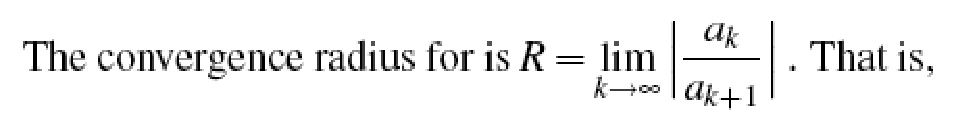
\includegraphics[width=0.55\textwidth]{latex}}}
\subfigure[由~Word软件生成的~.doc~格式行内公式]{\label{fig:subfig:word}
                \fbox{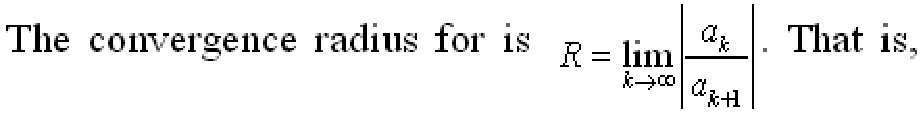
\includegraphics[width=0.55\textwidth]{word}}}
\subfigure[由~Word软件生成的~.pdf~格式行内公式]{\label{fig:subfig:pdf}
                \fbox{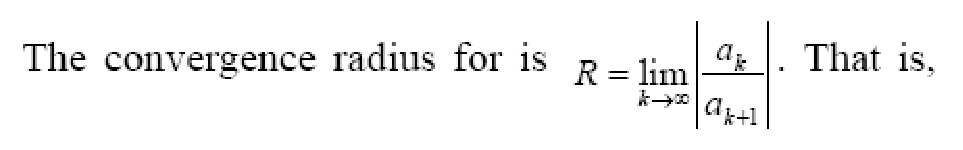
\includegraphics[width=0.55\textwidth]{pdf}}}

\caption{由~\LaTeX~和~Word~生成的~3~种行内公式屏显效果}\label{fig:hangju}
\vspace{-1em}
\end{figure}

这三幅图分别为~\LaTeX~和~Word~生成的行内公式屏显效果,从图中可看出,在~\LaTeX~文本含有公式的行内,在正文与公式之间对接工整,行距不变;而在~Word~文本含有公式的行内,在正文与公式之间对接不齐,行距变大。因此从这一点来说,
\LaTeX~系统在数学公式的排版上具有很大优势。

\LaTeX~提供的行内公式最简单、最有效的方法是采用~\TeX~本来的标记———开始和结束标记都写作~\$,例如本段开始的例子可由下面的输入得到。
\verb|$f(x)=\int_{a}^{b}\frac{\sin{x}}{x}\mathrm{d}x$|

\section{行间公式}
位于两行之间的公式称为行间公式,每个公式都是一个单独的段落,例如
\[\int_a^b{f\left(x\right)\mathrm{d}x}=\lim_{\left\|\Delta{x_i}\right\|\to 0}\sum_i{f\left(\xi_i\right)\Delta{x_i}}\]
除人工编号外,\LaTeX~各种类型行间公式的标记见表~\ref{tab:eqtag}。
\begin{table}[htbp]
\caption{各种类型行间公式的标记}\label{tab:eqtag}
\vspace{0.5em}\centering\wuhao
\begin{tabularx}{\textwidth}{cll}
\toprule
& 无编号 & 自动编号\\
\midrule
单行公式& \verb|\begin{displaymath}... \end{displaymath}|& \verb|\begin{equation}... \end{equation}|\\
        & 或~\verb|\[...\]| & \\
多行公式& \verb|\begin{eqnarray*}... \end{eqnarray*}|& \verb|\begin{eqnarray}... \end{eqnarray}|\\
\bottomrule
\end{tabularx}
\end{table}

另外,在自动编号的某行公式行尾添加标签~\verb|\nonumber|,可将该行转换为无编号形式。

行间多行公式需采用~\verb|eqnarray|~或~\verb|eqnarray*|~环境,它默认是一个列格式为~\verb|rcl|~的~3~列矩阵,并且中间列的字号要小一些,因此通常只将需要对齐的运算符号(通常为等号“=”)置于中间列。

\section{可自动调整大小的定界符}
若在左右两个定界符之前分别添加命令~\verb|\left|~和~\verb|\right|,则定界符可根据所包围公式大小自动调整其尺寸,这可从式(\ref{nodelimiter})和式(\ref{delimiter})中看出。
\begin{equation}\label{nodelimiter}
(\sum_{k=\frac12}^{N^2})
\end{equation}
\begin{equation}\label{delimiter}
\left(\sum_{k=\frac12}^{N^2}\right)
\end{equation}
式(\ref{nodelimiter})和式(\ref{delimiter})是在~\LaTeX~中分别输入如下代码得到的。
\begin{verbatim}
(\sum_{k=\frac12}^{N^2})
\left(\sum_{k=\frac12}^{N^2}\right)
\end{verbatim}
\verb|\left|~和~\verb|\right|~总是成对出现的,若只需在公式一侧有可自动调整大小的定界符,则只要用“.”代替另一侧那个无需打印出来的定界符即可。

若想获得关于此部分内容的更多信息,可参见~\href{http://tug.ctan.org/cgi-bin/ctanPackageInformation.py?id=voss-mathmode}{Math mode}~文档的第~8~章“Brackets, braces and parentheses”。

\section{数学重音符号}
数学重音符号通常用来区分同一字母表示的不同变量,输入方法如下(需要调用~\verb|amsmath|~宏包):

\vspace{0.5em}\noindent\wuhao\begin{tabularx}{\textwidth}{Xc|Xc|Xc}
 \verb|\acute| & $\acute{a}$ & \verb|\mathring| & $\mathring{a}$ & \verb|\underbrace| & $\underbrace{a}$ \\
 \verb|\bar| & $\bar{a}$ & \verb|\overbrace| & $\overbrace{a}$ & \verb|\underleftarrow| & $\underleftarrow{a}$ \\
 \verb|\breve| & $\breve{a}$ & \verb|\overleftarrow| & $\overleftarrow{a}$ & \verb|\underleftrightarrow| & $\underleftrightarrow{a}$ \\
 \verb|\check| & $\check{a}$ & \verb|\overleftrightarrow| & $\overleftrightarrow{a}$ & \verb|\underline| & $\underline{a}$ \\
 \verb|\dddot| & $\dddot{a}$ & \verb|\overline| & $\overline{a}$ & \verb|\underrightarrow| & $\underrightarrow{a}$ \\
 \verb|\ddot| & $\ddot{a}$ & \verb|\overrightarrow| & $\overrightarrow{a}$ & \verb|\vec| & $\vec{a}$ \\
 \verb|\dot| & $\dot{a}$ & \verb|\tilde| & $\tilde{a}$ & \verb|\widehat| & $\widehat{a}$ \\
 \verb|\grave| & $\grave{a}$ & \verb|\underbar| & $\underbar{a}$ & \verb|\widetilde| & $\widetilde{a}$ \\
 \verb|\hat| & $\hat{a}$
\end{tabularx}\vspace{0.5em}
\xiaosi 当需要在字母~$i$~和~$j$~的上方添加重音符号时,为了去掉这两个字母顶上的小点,这两个字母应该分别改用~\verb|\imath|~和~\verb|\jmath|。

如果遇到某些符号不知道该采用什么命令能输出它时,则可通过~\href{http://detexify.kirelabs.org/classify.html}{Detexify$^2$~网站}来获取符号命令。若用鼠标左键在此网页的方框区域内画出你所要找的符号形状,则会在网页右方列出和你所画符号形状相近的~5~个符号及其相对应的~\LaTeX~输入命令。若所列出的符号中不包括你所要找的符号,还可通过点击“Select from the complete list!”的链接以得分从低到高的顺序列出所有符号及其相对应的~\LaTeX~输入命令。

最后,建议大家还以~\href{http://tug.ctan.org/cgi-bin/ctanPackageInformation.py?id=voss-mathmode}{Math mode}~这篇~pdf~文档作为主要参考。若要获得最为标准、美观的数学公式排版形式,可以查查文档中是否有和你所要的排版形式相同或相近的代码段,通过修改代码段以获得你所要的数学公式排版形式。


%% !Mode:: "TeX:UTF-8"

\chapter{罗列和定理环境使用方法}

\section{单层罗列环境}
湖南大学学位论文一般可采用两种罗列环境:一种是并列条目有同样标签的~\verb|itemize|~罗列环境,另一种是具有自动排序编号符号的~\verb|enumerate|~罗列环境。这两种罗列环境的样式参数可参考图~\ref{fig:list}。
\begin{figure}[htbp]
\centering
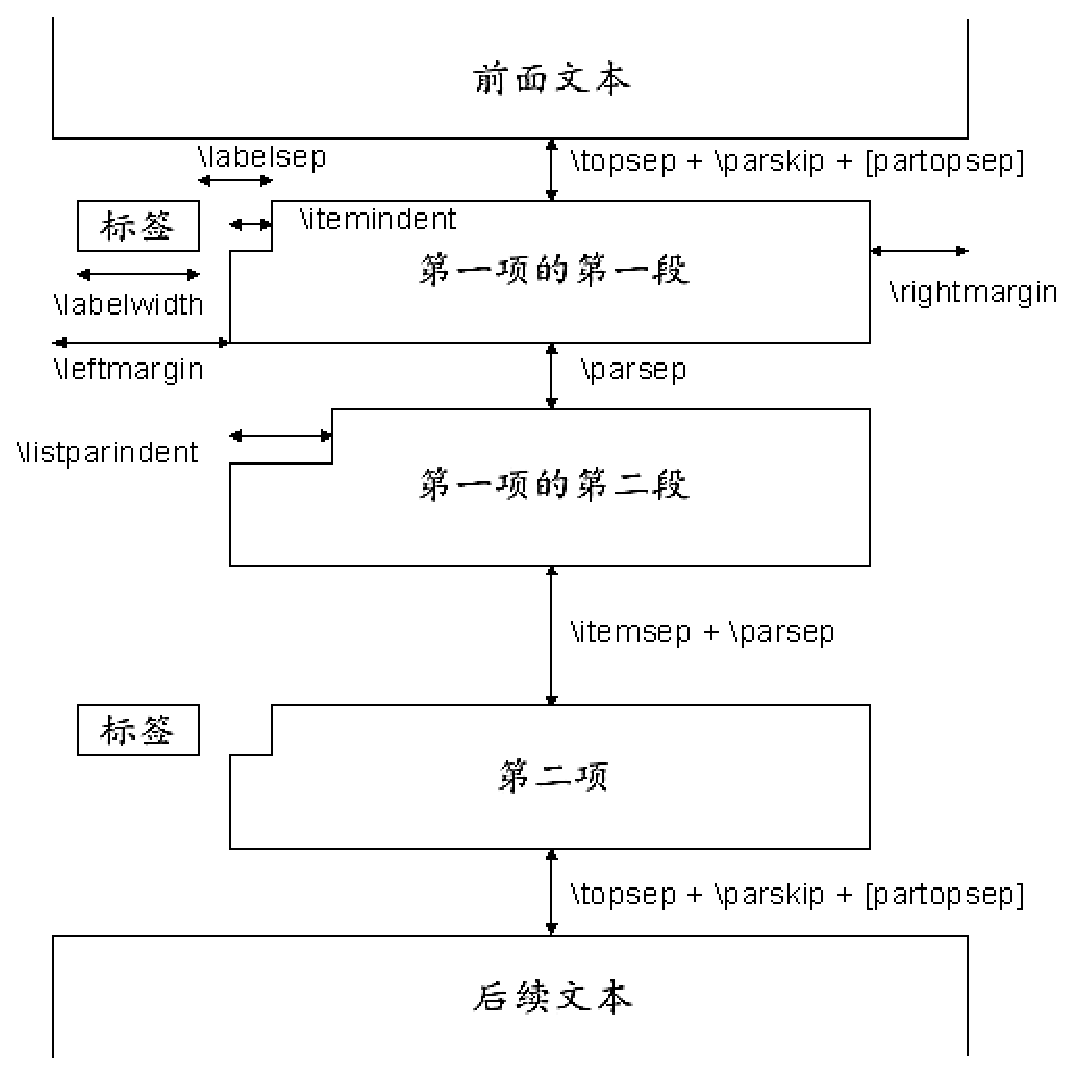
\includegraphics[width = 0.6\textwidth]{list}
\caption{罗列环境参数示意图}\label{fig:list}\vspace{-1em}
\end{figure}

通过调用~enumitem~宏包可以很方便地控制罗列环境的布局,其~format.tex~文件中的~\verb|\setitemize|~和~\verb|\setenumerate|~命令分别用来设置~\verb|itemize|~和~\verb|enumerate|~环境的样式参数。采用~\verb|itemize|~单层罗列环境的排版形式如下:

\begin{itemize}
\item 第一个条目文本内容
\item 第二个条目文本内容
\item 第三个条目文本内容
\end{itemize}

其代码如下

\begin{verbatim}
\begin{itemize}
  \item 第一个条目文本内容
  \item 第二个条目文本内容
  ...
  \item 第三个条目文本内容
\end{itemize}
\end{verbatim}

采用~\verb|enumerate|~单层罗列环境的排版形式如下:

\begin{enumerate}
\item 第一个条目文本内容
\item 第二个条目文本内容
\item 第三个条目文本内容
\end{enumerate}

其代码如下

\begin{verbatim}
\begin{enumerate}
  \item 第一个条目文本内容
  \item 第二个条目文本内容
  ...
  \item 第三个条目文本内容
\end{enumerate}
\end{verbatim}



\section{定理环境}

\begin{definition}[谱半径]\label{def:def1}
  称~$n$~阶方阵~$\mathbf{A}$~的全体特征值~$\lambda_1,\cdots,\lambda_n$~组成的集合为~$\mathbf{A}$~的谱,称
  $$\rho(\mathbf{A})=\max{\{|\lambda_1|,\cdots,|\lambda_n|\}}$$
\end{definition}
\begin{theorem}[相似充要条件]\label{lemma:l1}
  方阵$A$和$B$相似的充要条件是:~$A$~和~$B$~有全同的不变因子。
\end{theorem}
\begin{corollary}[推论1]\label{cor:cor1}
在赋范空间~$(X,\|\cdot\|)$~上定义~$d(x,y)=\|x-y\|$, 对任意~$x,y\in X$,~则~$(X,d)$~是距离空间。
\end{corollary}
\begin{proof}
  只需证明~$d(x,y)$~是距离。
\end{proof}
\newpage

定义代码如下:
\begin{verbatim}
 \begin{definition}[谱半径]\label{def:def1}
  称~$n$~阶方阵~$\mathbf{A}$~的全体特征值
  $\lambda_1,\cdots,\lambda_n$组成的集合为~$\mathbf{A}$~的谱,称
  $$\rho(\mathbf{A})=\max{\{|\lambda_1|,\cdots,|\lambda_n|\}}$$
\end{definition}
\end{verbatim}
\noindent\hrule

\vspace{0.1em}\noindent\hrule
\vspace{1em}
定理代码如下:
\begin{verbatim}
\begin{theorem}[相似充要条件]\label{lemma:l1}
  方阵$A$和$B$相似的充要条件是:$A$和$B$有全同的不变因子。
\end{theorem}
\end{verbatim}
\noindent\hrule\vspace{0.1em}

\noindent\hrule
\vspace{1em}
推论和证明代码如下:
\begin{verbatim}
\begin{corollary}[推论1]\label{cor:cor1}
在赋范空间~$(X,\|\cdot\|)$~上定义$d(x,y)=\|x-y\|$,
对任意$x,y\in X$,则$(X,d)$是距离空间。
\end{corollary}
\begin{proof}
  只需证明$d(x,y)$是距离。
\end{proof}
\end{verbatim}
\noindent\hrule\vspace{1em}

定理定义[]中是可选参数,用来说明定理的名称。其他环境格式书写与上面定理、定义、推论格式相同,可自己调用其他环境。
若需要书写定理定义等内容,而且带有顺序编号,需要采用如下环境。除了~\verb|proof|~环境之外,其余~9~个环境都可以有一个可选参数作为附加标题。

\begin{center}
\vspace{0.5em}\noindent\wuhao\begin{tabularx}{0.7\textwidth}{lX|lX}
定理 & \verb|theorem|~环境 & 定义 & \verb|definition|~环境 \\
例 & \verb|example|~环境 & 算法 & \verb|algorithm|~环境 \\
公理 & \verb|axiom|~环境 & 命题 & \verb|proposition|~环境 \\
引理 & \verb|lemma|~环境 & 推论 & \verb|corollary|~环境 \\
注解 & \verb|remark|~环境 & 证明 & \verb|proof|~环境 \\
\end{tabularx}
\end{center} 
% !Mode:: "TeX:UTF-8"

\addcontentsline{toc}{chapter}{结论与展望} %添加到目录中
\chapter*{结论与展望}
随着科学技术的进步,超大规模集成电路的发展速度日新月异。芯片集成度以及复杂度的急剧上升增加了制造合格芯片的困难。为了确保芯片的故障覆盖率达标,需要大量的测试数据对其进行检测。庞大的测试数据增加了硬件代价以及测试时间,一种卓有成效的方法就是对测试数据进行压缩。近年来有学者提出了一种拆分压缩技术,此技术将原测试集拆分成为主分量集(在本文中由基向量生成)以及残分量集,进一部提高压缩率。主分量的选取直接影响最终的压缩率,本文在拆分压缩的基础上,对如何生成基向量展开了研究。

第一章绪论,介绍了集成电路发展的背景以及电路测试的相关先修知识,同时就国内外研究现状进行分析,最后总结本文的组织结构。第二章主要就常用的压缩方法做了详细地介绍。第一部分讲解了编码压缩技术,包括游程编码、字典编码以及统计编码。第二部分就基于线性解压缩和基于广播扫描两种非编码压缩方法做出了相应的分析与阐述,最后介绍了拆分压缩技术和哈达码变换,并对哈达码变换的优缺点进行了分析。本文就是在拆分压缩技术的基础上通过挑选出合适的基向量进行数据压缩。

本文针对测试集自身特性,在拆分压缩技术中,针对基向量的生成算法提出了两个创新点主要有:

(1)采用预填充的策略对测试集进行处理。此方法首先对测试数据进行预填充,填充的方式有直接填充和策略填充两种,填充的目的是使测试集在当前编码规则下的压缩率更高,填充完毕后的测试集不存在无关位,然后以向量间距离最大最原则选取需要的基向量。由于本文使用的是拆分压缩技术,当原测试及中包含的码字0较多会有助于压缩率的提升,建议直接将无关位填充为码字0。实验结果表明,使用预填充的方式,RL-Huff编码的压缩率可达74.32\%,相比与对测试集进行直接编码,压缩率提高了11.75\%。通过和大多数压缩方法进行对比表明,对于大多数基准电路,使用本方法均可以获得较好的效果。

(2)提出了一种基于kmeans++聚类算法结合测试集生成基向量的方法。该方法通过步骤(1)消除原测试集中的无关位,然后对已填充的测试向量进行聚类,即相似的列向量我们将其归为一类,随后取当前聚类列向量每一位的均值作为聚类中心向量,并以每一个聚类中心向量为基准,将测试集中的每一个列向量与以获得的聚类中心向量进行对比,若欧几里得距离最小则归为一类,如此反复迭代,当聚类基本不再发生变化时,最终确定的聚类中心向量即为我们所求的基向量。实验结果表明,通过使用kmeans++算法生成的基向量来进行压缩, RL-Huff编码的平均压缩率可达76.30\%,与对测试集进行直接编码压缩相比平均压缩率提高了13.73\%,与哈达码相比,压缩率提高了4.45\%。同时本人使用此方法对大电路进行了测试,在FDR编码编码方式下,比对测试集直接压缩所获取的缩率高 6.06\%。由于基向量的选取的个数会直接影响最终的压缩率,为了更好的反映两者的对应关系,本人通过选取不同个数的基向量,计算出相应的压缩率,并绘画出其相应的折线图。

(3)将kmeans++聚类算法结合单轮位翻转算法进一步提高压缩率。此方法的主要思想是,先对原测试集进行预填充,利用kmeans++聚类算法找出所需的基向量并生成主分量集,然后对主分量集进行故障模拟检测出电路的部分故障,然后对原测试集也进行故障模拟,将主分量集能检测出故障对应的确定位转化成为无关位,并生成新的测试集。最后将新的原测试集与主分量集异或,得到新的残分量集,提升压缩率。本人基于多轮位翻转算法提出一种保留原主分量集合的单轮位翻转算法,使得在进行故障模拟时,所需要的硬件代价更小。结果表明使用位翻转算法结合kmeans++算法可以将平均压缩率相比于步骤(2)提高了7\%。

针对在拆分压缩技术中的基向量的生成算法研究,文中提出的三种方法虽然在取得了一定的成果,但仍然有不足和和厄待改进之处。现总结如下:

(1)本文在第三章使用采用预填充的策略对测试集进行处理,并且其取得了较好的效果,但是主要因为是因为基向量选取方式所导致的,在预填充的测试集中,如果选举基向量的策略为随机选取,而不是使用向量间距离最大原则为依据选取会对压缩率产生较大的影响,实验表明使用随机选取方式所达到的压缩率,与使用哈达码变换所达到的压缩率十分接近。虽然本文使用了据间距最大原则,但是第一列基向量的选取依旧是随机的,初始基向量的选取对实验结果的影响较为明显,因此预填充之后,对于基向量的选择还可以继续优化,减少随机选取带来的误差。

(2)本文第四章提出了一种基于kmeans++聚类算法结合测试集生成基向量的方法。该方法的基本思想是对已填充的测试向量进行聚类,以每一个聚类中心向量为基准,将测试集中的每一个列向量与以获得的聚类中心向量进行对比,若欧几里得距离最小则归为一类,如此反复迭代,当聚类基本不再发生变化时,基向量获取结束。由实验结果可知此方法能获取较高的压缩增益,但也有缺陷,第一kmeans++算法是一个以距离为基准的算法,简单易用,其缺点是无法确定聚类数目,需要事先设定,其次在聚类时初始基向量的选取也是随机的对实验结果也会存在一定的影响。综上所述,在聚类算法的选择上还有很大的空间,可能存在某种聚类算法可以直接确定原测试集聚类个数并且硬件代价也相对较小。

(3)本文第五章通过将kmeans++聚类算法结合位翻转算法来提高压缩率,此方法的主要思想是:对主分量集进行故障模拟检测出电路的部分故障,然将原测试集部分确定位转化为无关位,从而提升压缩率。虽说针对所有基准电路,此方法提升了较高的压缩率,但是本文中提及的翻转算法只翻转了一轮,并且翻转时使用的是贪婪算法,可能无法到达全局最优的效果,因此对翻转算法进一步优化增加可翻转的确定位,是一个可以研究的突破点,比如根据主分量集合的确定位情况设计相应的翻转算法,从而提高残分量的压缩率。

%%%%%%%%%% 正文部分内容  %%%%%%%%%%

%%%%%%%%%%  参考文献  %%%%%%%%%%
\defaultfont
\bibliographystyle{HNUThesis}
\phantomsection
\addcontentsline{toc}{chapter}{参考文献}          % 参考文献加入到中文目录
\nocite{*}                                        % 若将此命令屏蔽掉,则未引用的文献不会出现在文后的参考文献中。
\bibliography{reference}
% !Mode:: "TeX:UTF-8"
\addcontentsline{toc}{chapter}{致\quad 谢} %添加到目录中
\chapter*{致\quad 谢}

%湖南大学学位论文~\LaTeX~模板主要参考以下内容:
%\begin{itemize}
%  \item 天津大学~TJUThesis~硕博士学位论文模板
% \end{itemize}

%感谢~ChinaTeX~大神的无私帮助。
%
%谨将此论文模板,献给我们最爱的母校:湖南大学。
%
%\vspace*{1cm}
%本论文的工作是在我的导师[XXXX...] 教授的悉心指导下完成的,[XXXX...]
%
%教授严谨的治学态度和科学的工作方法给了我极大的帮助和影响。在此衷心感谢三年来[XXXX...] 老师对我的关心和指导。
%
%[XXXX...] 教授悉心指导我们完成了实验室的科研工作,在学习上和生活上都给予了我很大的关心和帮助,在此向[XXXX...] 老师表示衷心的谢意。
%
%[XXXX...] 教授对于我的科研工作和论文都提出了许多的宝贵意见,在此表示衷心的感谢。
%
%在实验室工作及撰写论文期间,[XXXX...] 、[XXXX...] 等同学对我论文中的[XXXX...] 研究工作给予了热情帮助,在此向他们表达我的感激之情。
%
%另外也感谢家人[XXXX...] ,他们的理解和支持使我能够在学校专心完成我的学业。
如果说人生是一首优美的乐曲,那么湖大的日子则是其中一个美妙的音符。三年前我成功考上了心心念念的湖大,一切都是那么新鲜,由于我是个跨专业的考生,在研究生期间我加倍努力,打实专业基础,在此期间由于结识了一批优秀的同学,让我对自己的人生有了规划与追求。这一路走来,有欢声笑语,也有挫败失落。三年的研究生时光即将结束,感谢陪我一起走过这段岁月的人儿,愿你们身体健康事事顺心,也同样希望你们的生活中,因为有我的存在可以带给你们一些欢乐与帮助。

首先,由衷地感谢我的导师xxx对我的悉心指导和多方关怀!老师对我的帮助不仅仅是学业上的指导,更是设计到了生活中的方方面面,老师是一个很开明的人,对于学生想做的事情只要对人生、学业有益,均会全力支持。老师是个很睿智的人,对于生活中遇到的困难,均会加以开导,每次与老师谈话完毕总是豁然开朗。同时老师是一个很严谨的人,对待工作一丝不苟,以学生学业为重,为了提升教学质量,经常想各种方法来激起学生的学习积极性与主动性。三年前,考研初试刚刚结束,我就联系了老师,知道我是跨考生后老师并没有嫌弃我基础薄弱,反而悉心指导我该看什么书籍,该朝哪方面努力,在此由衷感谢导师这三年对我的帮助与关照,您的悉心教导足矣让我受用终身。

感谢我的校外导师xxx,每次遇到不会解决的问题时,都会很耐心地给我解答。特别是择业期间,你给我提供了很多宝贵意见,结合我自身实际情况给我分析了各个企业的优劣,最终使我获得了心仪的工作。祝愿文吉刚老师在今后的每一天身体健康、事事顺心。

感谢实验室的老师以及各位同学,感谢xxx老师、xxx老师、xxx博士、xxx博士给我的指导与帮助。感谢师弟xxx,遇到问题时和你探讨总能激发灵感。感谢幽默室友xxx,因为你让我的生活变得十分有趣。感谢大佬室友xxx,是你让我了解到自己离优秀的距离还相当遥远。感谢好朋友xxx,每次和你交流我都能获得灵感。还要特别感谢xxx同学对我的帮助。

尤其要感谢我的母亲,谢谢你一直以来的支持与鼓励,教我明辨是非,教我如何做一个大写的人。感谢我的父亲,感谢您为家庭的默默付出,任劳任怨,因为您我才有机会顺利完成学业,拥有更精彩的人生。在以后的工作与生活中,我会带着你们的期望继续前行,愿你们身体健康,事事顺心。

最后,感谢参与盲审以及答辩的各位专家和老师,谢谢你们提出的宝贵意见。












               % 致谢
% !Mode:: "TeX:UTF-8"

\addcontentsline{toc}{chapter}{附录A  发表论文和参加科研情况说明}
\chapter*{附录A~~~~发表论文和参加科研情况说明}
\setlength{\parindent}{0em}
\begin{publist}
%\item XXX,XXX. Density and Non-Grid based Subspace Clustering via Kernel Density Estimation[C]. ECML-PKDD 2012, Bristol, UK.(Submitted, Under review)
\item Fifth author. Intrusion Detection for In-vehicle Network by Using Single GAN in Connected Vehicles[J]. Journal of Circuits, Systems, and Computers, .(has been accepted).
\item second author. 基于测试集主成分的变换--拆分法提高编码压缩率.电子测量与仪器学报.
\item 软件著作权:xxx. PRE聚源集成电路测试向量压缩软件. 登记号:2020SR0199298.
\end{publist}

\vfill
\hangafter=1\hangindent=2em\noindent

\setlength{\parindent}{2em}
                   % 发表论文和参加科研情况说明
\clearpage
\end{CJK*}                                        % 结束中文字体使用
\end{document}                                    % 结束全文
